% !TEX encoding = UTF-8 Unicode
\chapter{Methods} \label{chap-methods}

\section{Disturbance models} \label{sec:disturbance-models}

\subsection{Randomly-occurring deterministic disturbances} \label{sec:RODD}

\Acrlong{RODD}s (\acrshort{RODD}s) \citep{macgregor_duality_1984} are a family of stochastic process models suitable for simulating various types of infrequently-occurring disturbances in discrete-time.  The structure of the \gls{RODD} model is
\begin{equation} \label{eq:RODD}
	p(k) = \frac{B(q^{-1})}{A(q^{-1})} w_p(k),
\end{equation}
where $p(k)$ is the generated disturbance signal, $A(q^{-1})$ and $B(q^{-1})$ are polynomial functions of the backward shift operator, $q^{-1}$, and $w_p(k)$ is a random variable generated by a switching system.
\nomenclature{$p(k)$}{disturbance signal at time $k$}%
\nomenclature{$q^{-1}$}{backward shift operator}%
\nomenclature{$A(q^{-1})$}{\acrshort{RODD} model parameter: polynomial function of the backward shift operator}%
\nomenclature{$B(q^{-1})$}{\acrshort{RODD} model parameter: polynomial function of the backward shift operator}%
\nomenclature{$w_p(k)$}{random shock signal at time $k$}%
% One way to make links: \hyperlink{sym.pk}{$p(k)$}.

To generate randomly-occurring disturbances, the switching system,
\begin{equation} \label{eq:wpk1} 
	w_p(k) \sim 
	\begin{cases*}
		0 & with probability $1-\varepsilon$, \\
		\mathcal{N}\left( 0, \sigma_{w_p}^2 \right) & with probability $\varepsilon$,
	\end{cases*}
\end{equation}
\nomenclature{$\varepsilon$}{\acrshort{RODD} model parameter: probability of a random shock}%
may be used, where $w_p(k)$ is either 0 or is sampled from the normal distribution, $\mathcal{N}(0,\sigma_{w_p}^2)$, with mean zero and variance $\sigma_{w_p}^2$.  When the probability $\varepsilon$ is low ($\varepsilon<<1$), this system produces infrequent shocks.
\nomenclature{$\mathcal{N}(\mu,\sigma^2)$}{normal distribution with mean $\mu$ and variance $\sigma^2$}%

Alternatively, a mixture of two distributions may be used \citep{robertson_detection_1995}:
\begin{equation} \label{eq:wpk2}
w_p(k) \sim 
	\begin{cases*}
		\mathcal{N}\left(0, \sigma_{w_p}^2\right) & with probability $1-\varepsilon$, \\
		\mathcal{N}\left(0, b^2\sigma_{w_p}^2\right) & with probability $\varepsilon$.
	\end{cases*}
\end{equation}
\nomenclature{$\sigma_{w_p}$}{\acrshort{RODD} model parameter: standard deviation of the persistent noise component of the random shock variable}%
\nomenclature{$b$}{\acrshort{RODD} model parameter: variance of the random shocks divided by the variance of the persistent noise}%
% Don't think this is necessary to define:
%\nomenclature{$\sigma_{w_p}^2$}{variance of the persistent noise component of the random shock variable}%

In this formulation, $\sigma_{w_p}$ represents the standard deviation of the \hl{persistent} noise in periods between random shocks and $b$ is typically large so that the magnitude of the shocks is many times greater than $\sigma_{w_p}$. One benefit of \eqref{eq:wpk2} is that the distribution of $w_p(k)$ is conditionally Gaussian, whereas in \eqref{eq:wpk1} it has a non-smooth (i.e. degenerate) probability density function.

Figure \ref{fig:wpk-pdf} illustrates the probability density of $w_p(k)$ in the case of \eqref{eq:wpk2} with $\sigma_{w_p}=0.01$, $b=100$, and $\varepsilon=0.01$. Although it is difficult to discern from the plot, this is a mixture distribution with two components. The component that generates the infrequent shocks is barely visible because of its low probability. In this example, 99 percent of the probability lies within a narrow range ($-0.036 < w_p(k) < 0.036$). However, the shocks, which occur with probability 0.01, have much higher amplitude ($b\sigma_{w_p}=1$).

\begin{figure}[ht]
	\centering
	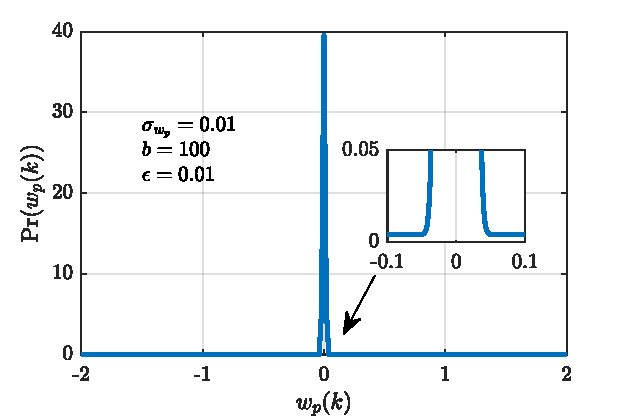
\includegraphics[width=11.5cm]{wpk-pdf-4.pdf}
	\caption{Probability density of a random shock signal}
	\label{fig:wpk-pdf}
\end{figure}

When dealing with a system having more than one \gls{RODD}, where each random shock is independent, the notation is
\begin{equation} \label{eq:wpik2}
	w_{p,i}(k) \sim 
	\begin{cases*}
		\mathcal{N}\left(0, \sigma_{w_p,i}^2\right) & with probability $1-\varepsilon_i$, \\
		\mathcal{N}\left(0, b_i^2\sigma_{w_p,i}^2\right) & with probability $\varepsilon_i$,
	\end{cases*}
\end{equation}
where $i \in \left\{1, 2, ..., n_p\right\}$.
\nomenclature{$n_p$}{number of independent random shock disturbance processes}%

The choice of $A(q^{-1})$ and $B(q^{-1})$ in \eqref{eq:RODD} determines the nature of the \gls{RODD}. For example, if $B(q^{-1})=1$ and $A(q^{-1})=1-q^{-1}$, $p(k)$ will be a random-walk process with infrequent, large step changes.

% Add symbol to glossary
Using $\nabla$ to denote $1-q^{-1}$, the \gls{RODD} \textit{step-disturbance} process can be defined as
\nomenclature{$\nabla$}{defined as $1-q^{-1}$}%
\begin{equation} \label{eq:RODD-step}
	p(k) = \frac{1}{\nabla}w_p(k).
\end{equation}

A \gls{RODD} \textit{ramp-disturbance}, consisting of a series of ramps with randomly-occurring changes in slope, may be generated using
\begin{equation} \label{eq:RODD-ramp}
	p(k) = \frac{1}{\nabla^2}w_p(k).
\end{equation}

A \gls{RODD} consisting of randomly-occurring decaying exponential changes may be generated using
\begin{equation} \label{eq:RODD-exp}
	p(k) = \frac{1}{(1-a_1q^{-1})\nabla}w_p(k),
\end{equation}
where  $0<a_1<1$. Note that $a_1=0$ corresponds to the case of a \gls{RODD} step disturbance \eqref{eq:RODD-step} and $a_1=1$ to that of a \gls{RODD} ramp disturbance \eqref{eq:RODD-ramp}. 

An equivalent state-space representation of \eqref{eq:RODD-exp} is
\begin{equation} \label{eq:RODD-ss}
	\begin{split}
		\mathbf{x}_p(k+1) & =\left[\begin{array}{cc}
			1 & 1 \\
			0 & a_1
		\end{array}\right] \mathbf{x}_p(k) +\left[\begin{array}{cc}
			0 \\
			1
		\end{array}\right] w_p(k) \\
		p(k) & =\left[\begin{array}{cc}
			1 & 0
		\end{array}\right] \mathbf{x}_p(k),
	\end{split}
\end{equation}
\nomenclature{$\mathbf{x}_p(k)$}{disturbance model states at time $k$}%
where $\mathbf{x}_p(k) \in \mathbb{R}^2$ is the state vector.

A disturbance with a combination of different \gls{RODD}s is also possible.  For example, a state-space representation of a \gls{RODD} consisting of step changes and ramps is
\begin{equation} \label{eq:RODD-step-ramp}
	\begin{split}
		\mathbf{x}_p(k+1) & =\left[\begin{array}{cc}
			1 & 1 \\
			0 & 1
		\end{array}\right] \mathbf{x}_p(k) +\left[\begin{array}{cc}
			1 & 0 \\
			0 & 1
		\end{array}\right] \mathbf{w}_p(k) \\
		p(k) & =\left[\begin{array}{cc}
			1 & 0
		\end{array}\right] \mathbf{x}_p(k),
	\end{split}
\end{equation}

where $\mathbf{w}_p(k)$ is a vector of two independent random shock signals generated by \eqref{eq:wpik2}. Simulated examples of these \gls{RODD}s are presented in figures \ref{fig:rodd-sim-plots} and \ref{fig:rodd-sim-plot2}.

\subsection{Hidden Markov models} \label{sec:HMM}

\textit{Hidden Markov models} (\gls{HMM}) can be used to simulate a more diverse set of switching behaviours than those of the \gls{RODD} model described in the previous section \citep{wong_realistic_2009}. A Markov process or Markov chain is a stochastic model used to describe a sequence of discrete events for which the probability of future events depends only on the current state. A \gls{HMM} is a Markov model with states that are not fully observable (i.e. hidden or observed with a measurement error).

To illustrate the basic concept, the state of the random shock process \eqref{eq:wpk2} \hl{may be defined} as a Markov model with a state that has two possible values,
\begin{equation} \label{eq:gamma-k}
	\gamma(k) \in \{0,1\}.
\end{equation}
\nomenclature{$\gamma(k)$}{random shock indicator at time $k$}%
$\gamma(k)=1$ represents a shock at time $k$, and $\gamma(k)=0$ means no shock occurs. The switching of $\gamma(k)$ can then be defined by a \textit{transition matrix}, $\Pi$, which describes the probabilities of transitioning from every mode at time $k$ to every mode at time $k+1$:
\begin{equation} \label{eq:Pi}
	\begin{aligned}
	\Pi &= \left(\pi_{ij} \forall i,j\in \{1,2,...,n_j\}\right) \\
	\pi_{ij} &= \Pr\left( \gamma(k)=j-1 \mid \gamma(k-1)=i-1 \right),
	\end{aligned}
\end{equation}
\nomenclature{$\Pr(A \mid B)$}{probability of an event $A$ given an event $B$}%
\nomenclature{$n_j$}{number of modes or models of a switching system}%
where $n_j$ is the number of possible system modes and $\pi_{ij}$ is the probability that the system mode at time $k$ is $j-1$ given that it was $i-1$ at time $k-1$.

In the case of the random shock, $n_j=2$ and the equivalent Markov process has the transition probability matrix
\nomenclature{$\Pi_{w_{p}}$}{transition probability matrix of the disturbance process $w_p$}%
\begin{equation} \label{eq:Pi-RODD-step}
	\Pi_{w_{p}} = \begin{bmatrix}
	1-\varepsilon & \varepsilon \\
	1-\varepsilon & \varepsilon
	\end{bmatrix}.
\end{equation}
Since $w_{p}(k)$ is an independent random variable, it does not depend on the previous state, $\gamma(k-1)$. Therefore, the rows of $\Pi_{w_{p}}$ are identical.

The use of the Markov model thus allows transition probabilities that do depend on the previous state. For example, consider a disturbance where the signal switches infrequently between samples from two or more distributions with different parameters. The probabilities of switching from one distribution to another may be different. Such a disturbance process could be simulated with a hidden Markov model by conditioning the distribution from which $w_p(k)$ is sampled on a Markov state, $r(k)$, with an arbitrary number of modes,
\nomenclature{$r(k)$}{mode indicator of a switching system at time $k$}%
\begin{equation} \label{eq:mog-example}
	\begin{split}
		w_p(k) \sim 
		\begin{cases*}
			\mathcal{N}\left(\mu_{w_p,1}, \sigma_{w_p,1}\right) & if $r(k)=1$, \\
			\mathcal{N}\left(\mu_{w_p,2}, \sigma_{w_p,2}\right) & if $r(k)=2$, \\
			... & ...\\
			\mathcal{N}\left(\mu_{w_p,n_j}, \sigma_{w_p,n_j}\right) & if $r(k)=n_j$.
		\end{cases*} \\
	\Pr(r(k)=j-1 \mid r(k-1)=i-1)=\pi_{ij} \forall i,j \in {1,2,...,n_j}
	\end{split}
\end{equation}

To make the notation more concise, allow the value of any time-varying discrete variable such as $\sigma_{w_p} \in \left\{\sigma_{w_p,1}, \sigma_{w_p,2},..., \sigma_{w_p,n_j}\right\}$, to be determined by the value of the Markov state $r(k)$. Thus,
\begin{equation} \label{eq:A-selection}
	\sigma_{w_p}(r(k)) = 
	\begin{cases*}
		\sigma_{w_p,1} & if $r(k)=1$, \\
		\sigma_{w_p,2} & if $r(k)=2$, \\
		... & ...\\
		\sigma_{w_p,n_j} & if $r(k)=n_j$.
	\end{cases*}
\end{equation}

With this notation, \eqref{eq:mog-example} can be written concisely as
\begin{equation} \label{eq:mog-example2}
	\begin{aligned}
		w_p(k) &\sim \mathcal{N}\left(\mu_{w_p}(r(k)), \sigma_{w_p}(r(k))\right) \\
		\Pr(r(k) &= j-1 \mid r(k-1)=i-1)=\pi_{ij} \forall i,j \in {1,2,...,n_j}.
	\end{aligned}
\end{equation}
where $\mu_{w_p}\in\left\{\mu_{w_p,1},\mu_{w_p,2},...,\mu_{w_p,n_j}\right\}$. This model is known as a \textit{mixture of Gaussians} and can be considered a special-case of a HMM-based disturbance model \citep{wong_disturbance_2007}.

A \gls{HMM} disturbance process can be represented by a \textit{Markov jump linear system} (\acrshort{MJLS}) \citep{costa_discrete-time_2005}. The state-space representation with time-varying system matrices $\mathbf{A}(\gamma(k))$, $\mathbf{B}(\gamma(k))$, and $\mathbf{C}(\gamma(k))$, and a vector of independent time-varying random shock inputs, $\mathbf{w}_p(k)$ \eqref{eq:mog-example2}, is defined
\begin{equation} \label{eq:MJLS}
	\begin{aligned}
	\mathbf{x}_p(k+1) &= \mathbf{A}(r(k)) \mathbf{x}_p(k) + \mathbf{B}(r(k))\mathbf{w}_p(k) \\
	\mathbf{p}(k) &= \mathbf{C}(r(k)) \mathbf{x}_p(k) + \mathbf{e}_p(k).
	\end{aligned}
\end{equation}

Note that $\mathbf{e}_p(k)$ may also be a switching random variable if desired. \eqref{eq:MJLS} is a versatile model suitable for representing and simulating a diverse family of stochastic disturbances.

\subsection{Bounded disturbances} \label{sec:bounded}

The \textit{bounded random walk} (\gls{BRW}) is a stochastic process proposed by \cite{nicolau_stationary_2002}. The discrete-time version is defined by the difference equation
\begin{equation} \label{eq:brw}
		p(k+1) = p(k) + a(p(k)) + e(k),
\end{equation}
where $e(k)$ is a random noise with variance $\sigma_e^2$, and $a(\cdot)$ is a function defined as
\nomenclature{$a(\cdot)$}{additive bias function used in the \acrshort{BRW}}%
\nomenclature{$\alpha_{1}$}{\acrshort{BRW} parameter}%
\nomenclature{$\alpha_{2}$}{\acrshort{BRW} parameter}%
\nomenclature{$\tau$}{\acrshort{BRW} parameter}%
\begin{equation}
	a(x) = e^{\beta}\left(e^{-\alpha_{1}\left(x - \tau\right)} - e^{\alpha_{2}\left(x - \tau\right)}\right),
\end{equation}
where $\beta$, $\alpha_{1}$, and $\alpha_{2}$ are constants.  From \eqref{eq:brw} it can be deduced that
\begin{equation}
	\mathbb{E}\{p(k+1)|p(k)\} = p(k) + a(p(k)).
\end{equation}

Therefore, $a(p(k))$ has the effect of an additive bias or time-varying adjustment to $p(k+1)$ that depends on $p(k)$. The shape of $a(\cdot)$ is determined by the constants $\alpha_{1}$,  $\alpha_{2}$, $\beta$, and $\tau$. Figure \ref{fig:brw-a} shows $a(p(k))$ in the case where $\tau=100$, $\beta=-15$, and $\alpha_{1}=\alpha_{2}=3$.  From this, it is clear that in the vicinity of $p(k)=\tau$, $a(p(k))\approx0$. When $a(p(k))=0$, \eqref{eq:brw} is the equation for a random walk. However, outside the neighbourhood, $p(k) \approx \tau$, $a(p(k))$ increases for low $p(k)$ or decreases for high $p(k)$. This has the effect of causing $p(k+1)$ to revert towards the mean ($\tau$) whenever $p(k)$ strays outside the neighbourhood. 
\begin{figure}[ht]
	\centering
	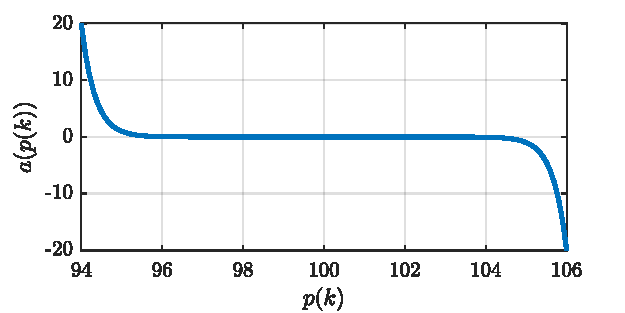
\includegraphics[height=5cm]{images/brw_a.pdf}
	\caption{A bounded random walk bias function}
	\label{fig:brw-a}
\end{figure}

Figure \ref{fig:brw-sim} shows a simulation of a \gls{BRW} with the above parameter values, and for comparison, an unbounded random walk (labelled `RW') generated with the same noise input. The dashed lines at $p(k)=95$ and $p(k)=105$ roughly indicate the location of the lower and upper bounds, which the \gls{BRW} only marginally exceeds.
\begin{figure}[ht]
	\centering
	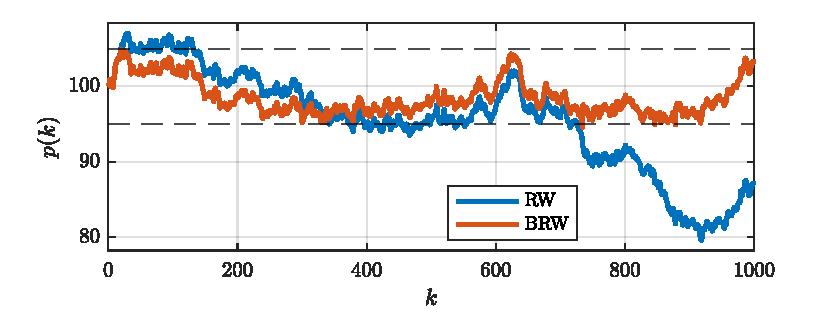
\includegraphics[height=5cm]{images/brw_sim.pdf}
	\caption{Examples of a bounded and unbounded random walk}
	\label{fig:brw-sim}
\end{figure}

Unlike a simple random walk, the \gls{BRW} is stationary. \cite{nicolau_stationary_2002} derived a formula for the form of the unconditional (i.e. stationary) probability distribution of the continuous-time \gls{BRW}. Figure \ref{fig:brw-pdf} shows the normalized stationary probability density of the \gls{BRW} defined above. For comparison, the probability density of a random walk process after 20 sample periods is also shown. It can be seen that there is a significant probability that the random walk would exceed the bounds of this \gls{BRW} after 20 sample periods. It can also be seen that the central part of the probability distribution of the \gls{BRW} is flat, indicating that all values within the bounds are equally likely after a large number of samples, similar to a uniform probability distribution.

%\begin{equation}
%	p_{BRW}(x) \propto \sigma^{-2} \exp \left\{-\frac{2 e^{k}}{\sigma^{2}}\left(\frac{e^{-\alpha_{1}(x-\tau)}}{\alpha_{1}}+\frac{e^{\alpha_{2}(x-\tau)}}{\alpha_{2}}\right)\right\}
%\end{equation}

\begin{figure}[ht]
	\centering
	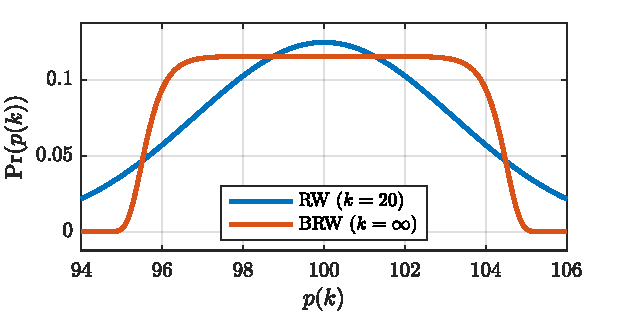
\includegraphics[height=5cm]{images/brw_pdf.pdf}
	\caption{Probability distributions of bounded and unbounded random walks}
	\label{fig:brw-pdf}
\end{figure}

However, the \gls{BRW} as defined in \eqref{eq:brw} is not guaranteed to be stable. Extreme values of $p(k)$ may cause $|a(p(k))|$ to be greater than $2|p(k)|$, which results in rapid divergence. This would cause computational errors in a numerical simulation. To avoid this, \cite{nicolau_stationary_2002} recommends adding a conditional regularizing step that forces reversion towards the mean, $\tau$, when the correction bias is too large. Instead of \eqref{eq:brw}, a conditional difference equation,
\begin{equation} \label{eq:brw-reg}
	p(k+1) = \begin{cases*}
		p(k) + a(p(k)) + e(k) & if $\left|a(p(k)) \right| < 2\left| p(k) - \tau \right|$, \\
		\tau + \phi(p(k) - \tau) + e(k) & if $\left|a(p(k)) \right| \geq 2\left| p(k) - \tau \right|$,
	\end{cases*}
\end{equation}
is used, where $\phi$ is a constant such that $0<\phi<1$. The size of $\phi$ determines how fast $p(k)$ reverts to $\tau$ when it is outside the stable region.

Since the \gls{BRW} has a non-Gaussian probability distribution, analysis of the properties of any dynamical system with a \gls{BRW} input is difficult. However, for simulation purposes, the \gls{BRW} is a simple and practical solution to the problem of bounding a random disturbance.

The \gls{BRW} concept could be extended to \gls{RODD}s. A \gls{RODD} step disturbance \eqref{eq:RODD-step} is a random walk with a switching noise variance \eqref{eq:wpk2}. The concern when trying to bound such a disturbance is the large step changes that occur infrequently. Since the probability of the shock, as well as the sign and amplitude of the step, are independent random variables, a \gls{RODD} step disturbance that happens to be at one of the bounds is as likely to step outside the bound as it is to step back inside the bounded region. The conditional regularity used in the \gls{BRW} \eqref{eq:brw-reg} would prevent any computational problems.


\section{State estimation} \label{sec:estimation}

State estimation is the task of estimating the values of the state variables of a dynamic model of a system given a set of measurements from the system. In process control applications, estimates of the states at the current time, or a prediction of their values at the next time instant, are required in real time (i.e. online) in order to calculate an appropriate control action.

Consider the diagram of an input-output system model in Figure \ref{fig:model_diag_uwvy}. Here, $\mathbf{u}(k)$ $\in \mathbb{R}^{n_u}$ is a vector of known input variables at time instant $k$, $\mathbf{w}(k)$ $\in \mathbb{R}^n$ is a vector of unmeasured state disturbances, $\mathbf{v}(k) \in \mathbb{R}^{n_y}$ is a vector of measurement errors, and $\mathbf{y}_M(k) \in \mathbb{R}^{n_y}$ is a vector of output measurements. The box represents a mathematical model that relates the inputs to the outputs and may be time-varying.
\nomenclature{$\mathbf{u}(k)$}{system inputs at time $k$}%
\nomenclature{$\mathbf{y}(k)$}{system outputs at time $k$}%
\nomenclature{$\mathbf{w}(k)$}{process disturbances at time $k$}%
\nomenclature{$\mathbf{v}(k)$}{measurement noises at time $k$}%
\begin{figure}[ht]
	\centering
	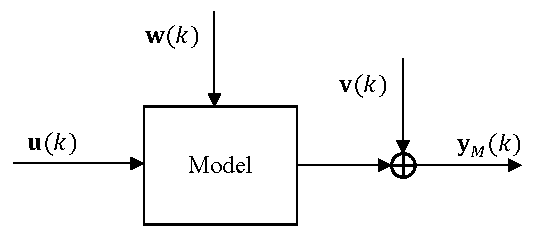
\includegraphics[width=8cm]{images/model_diag_uwvy.pdf}
	\caption{System model diagram}
	\label{fig:model_diag_uwvy}
\end{figure}

A convenient form in which to represent discrete-time, linear, possibly time-varying, dynamical system models for state estimation and control purposes, is the state-space representation
\begin{equation} \label{eq:ss_rep_uwy}
	\begin{aligned}
		\mathbf{x}(k+1) &= \mathbf{A}(k) \mathbf{x}(k) + \mathbf{B}(k) \mathbf{u}(k) + \mathbf{w}(k), \\
		\mathbf{y}_M(k) &= \mathbf{C}(k) \mathbf{x}(k) + \mathbf{v}(k).
	\end{aligned}
\end{equation}
\nomenclature{$\mathbf{x}(k)$}{system model states at time $k$}%
\nomenclature{$\mathbf{A}$}{transition matrix of the system model}%
\nomenclature{$\mathbf{B}$}{input matrix of the system model}%
\nomenclature{$\mathbf{C}$}{output matrix of the system model}%
where $\mathbf{x}(k)$ $\in \mathbb{R}^n$ is a vector of state variables, $\mathbf{A}(k) \in \mathbb{R}^{n \times n}$ is the state transition matrix at time $k$, $\mathbf{B}(k) \in \mathbb{R}^{n \times n_u}$ is the input matrix at time $k$, and $\mathbf{C}(k) \in \mathbb{R}^{n_y \times n}$ is the output matrix at time $k$. In this work, the system matrices are not time-varying and are therefore denoted $\mathbf{A}$, $\mathbf{B}$, and $\mathbf{C}$ in the remainder of this chapter.

The \textit{Kalman filter} \citep{kalman_new_1960} is the optimal estimator for a linear system in which the unmeasured disturbances and measurement errors are Gaussian random variables with mean values of zero. There are two commonly-used implementations of the Kalman filter, the \textit{prediction form} and the \textit{filtering form}. In the prediction form, the estimates of the states at the next time instant ($k+1$), given the information available at the current time ($k$) are calculated using
\begin{equation}
\begin{aligned} \label{eq:xkp1_hat_p}
	\mathbf{\hat{x}}(k+1 \mid k) &= \mathbf{\hat{x}}(k+1 \mid k-1) + \mathbf{K}_p(k) \big( \mathbf{y}_M(k) - \mathbf{\hat{y}}(k \mid k-1) \big) \\
	&= \mathbf{A}\mathbf{\hat{x}}(k \mid k-1) + \mathbf{B}\mathbf{u}(k) + \mathbf{K}_p(k) \big( \mathbf{y}_M(k) - \mathbf{C} \mathbf{\hat{x}}(k \mid k-1) \big)
\end{aligned}
\end{equation}
\nomenclature{$\mathbf{y}_M(k)$}{system output measurements at time $k$}%
where $\hat{\mathbf{x}}(k \mid k-1)$ is the prediction of the states at time $k$ that was made with the information available at the previous time instant, $k-1$, $\mathbf{y}_M(k)$ is the current measurement of the output, and $\mathbf{K}_p(k) \in \mathbb{R}^{n \times n_y}$ is a (possibly time-varying) correction gain.
\nomenclature{$\mathbf{K}_p(k)$}{correction gain of the Kalman filter (prediction form)}%

In the filtering form, which is used in this work, the estimated states and outputs at the current time are calculated given the information available at the current time using
\begin{equation} \label{eq:xkyk_hat}
	\begin{aligned}
		\mathbf{\hat{y}}(k \mid k-1) &= \mathbf{C} \mathbf{\hat{x}}(k \mid k-1) \\
		\mathbf{\hat{x}}(k \mid k) &= \mathbf{\hat{x}}(k \mid k-1) + \mathbf{K}(k) \big( \mathbf{y}_M(k) - \mathbf{\hat{y}}(k \mid k-1)  \big) \\
		\mathbf{\hat{y}}(k \mid k) &= \mathbf{C} \mathbf{\hat{x}}(k \mid k)
	\end{aligned}
\end{equation}
\nomenclature{$\hat{\mathbf{x}}(k \mid k-1)$}{predictions of system model states at time $k$ made with information available at time $k-1$}%
\nomenclature{$\mathbf{K}(k)$}{correction gain of the Kalman filter (filtering form)}%
where $\mathbf{K}(k)$ $\in \mathbb{R}^{n \times n_y}$ is a (possibly time-varying) correction gain. Instead of \eqref{eq:xkp1_hat_p}, the predictions of the states at the next time instant are calculated using
\nomenclature{$\hat{\mathbf{x}}(k+1 \mid k)$}{predictions of system modelstates at time $k+1$ made with information available at time $k$}%
\nomenclature{$\hat{\mathbf{x}}(k \mid k)$}{estimates of system model states at time $k$ made with information available at time $k$}%
\nomenclature{$\hat{\mathbf{y}}(k \mid k)$}{estimates of system outputs at time $k$ made with information available at time $k$}%
\begin{equation} \label{eq:xkp1_hat}
	\mathbf{\hat{x}}(k+1 \mid k) = \mathbf{A} \mathbf{\hat{x}}(k \mid k) + \mathbf{B} \mathbf{u}(k).
\end{equation}

An intuitive interpretation of the Kalman filter is that it takes the predictions of the states at time $k$ made in the previous time instant using the system model, and corrects them based on the difference between the current output measurement, $\mathbf{y}_M(k)$, and the output predicted by the model, $\mathbf{C} \mathbf{\hat{x}}(k \mid k-1)$. The correction step \eqref{eq:xkyk_hat} and prediction step \eqref{eq:xkp1_hat} are executed iteratively each time step, given a prior prediction of the states at time zero, $\mathbf{\hat{x}}(0 \mid -1)=\mathbf{\hat{x}}_0$.
\nomenclature{$\mathbf{\hat{x}}_0$}{Initial values of the estimates of the system states at time 0}%

Although the predicted states, $\hat{\mathbf{x}}(k \mid k-1)$, are identical in both forms of the Kalman filter, the use of the updated (i.e. \textit{a posteriori}) estimates, $\hat{\mathbf{x}}(k \mid k)$, in the filtering form instead of the predicted states leads to an optimal estimate taking account of all the information available. However, it should be noted that in some control applications, the prediction form is beneficial because the state predictions, $\hat{\mathbf{x}}(k+1 \mid k)$, are available one time step ahead.

To track a system with time-varying parameters, a dynamic estimator is needed with a time-varying correction gain. In the case of the filtering form of the Kalman filter, $\mathbf{K}(k)$ is calculated at each time instant using
\begin{equation} \label{eq:Kk}
	\mathbf{K}(k) = \mathbf{P}(k \mid k-1)\mathbf{C}^\intercal \mathbf{S}^{-1}(k),
\end{equation}
where $\mathbf{S}(k)$ is the output prediction error covariance matrix, which is given by
\nomenclature{$\mathbf{S}(k)$}{covariance of the output prediction errors at time $k$}%
\begin{equation} \label{eq:Sk}
	\mathbf{S}(k) = \mathbf{C}\mathbf{P}(k \mid k-1)\mathbf{C}^\intercal + \mathbf{R},
\end{equation}
\nomenclature{$\mathbf{P}(k \mid k-1)$}{predictions of the state estimation error covariance at time $k$ made with information available at time $k-1$}%
and $\mathbf{P}(k \mid k-1)$ is the state estimation error covariance matrix calculated in the previous time instant. $\mathbf{R}$, which is time invariant in this work, is the covariance matrix of the measurement noises,
\nomenclature{$\mathbf{R}$}{covariance of the measurement noises in the observer model}%
\begin{equation} \label{eq:R}
	 \mathbf{R} = \mathbb{E}\{ \mathbf{v}(k) \mathbf{v}^\intercal(k) \},
\end{equation}
\nomenclature{$\mathbb{E}\{\cdot\}$}{expectation operator}%
where $\mathbb{E}\{\cdot\}$ is the expectation operator.

The corrected error covariance may be calculated using
\nomenclature{$\mathbf{P}(k \mid k)$}{state estimation error covariance at time $k$ made with information available at time $k$}%
\begin{equation} \label{eq:Pk}
	\mathbf{P}(k \mid k) = \left( \mathbf{I}_n - \mathbf{K}(k) \mathbf{C} \right) \mathbf{P}(k \mid k-1),
\end{equation}
given an initial covariance estimate at time zero, $\mathbf{P}(0 \mid -1)=\mathbf{P}_0$.%
\nomenclature{$\mathbf{P}_0$}{Initial value of the state estimation error covariance at time 0}

However, to reduce numerical errors due to rounding, the computation of $\mathbf{P}(k \mid k)$ is carried out in this work using the Joseph stabilized version of \eqref{eq:Pk} {\citep{lewis_optimal_2008}
 \begin{equation} \label{eq:Pk-stab}
 	\mathbf{P}(k \mid k) = \left( \mathbf{I}_n - \mathbf{K}(k) \mathbf{C} \right ) \mathbf{P}(k \mid k-1) \left( \mathbf{I}_n - \mathbf{K}(k) \mathbf{C} \right )^\intercal + \mathbf{K}(k)  \mathbf{R} \mathbf{K}(k)^\intercal,
 \end{equation}
\nomenclature{$\mathbf{I}_n$}{the identity matrix ($n \times n$)}%
where $\mathbf{I}_n$ is the identity matrix.

The prediction of the error covariance at the next time instant is made using
\nomenclature{$\mathbf{P}(k+1 \mid k)$}{predictions of the state estimation error covariance at time $k+1$ made with information available at time $k$}%
\begin{equation} \label{eq:Pkp1}
	\mathbf{P}(k+1 \mid k) = \mathbf{A} \mathbf{P}(k \mid k)  \mathbf{A}^\intercal  + \mathbf{Q}(k),
\end{equation}
where $\mathbf{Q}(k)$ is the time-varying covariance of the process disturbances,
\nomenclature{$\mathbf{Q}(k)$}{covariance of the process disturbances in the observer model at time $k$}%
\begin{equation} \label{eq:Q}
	\mathbf{Q}(k) = \mathbb{E}\{ \mathbf{w}(k) \mathbf{w}^\intercal(k) \}.
\end{equation}

Algorithm \ref{alg:kf} defines the sequence of the Kalman filter calculations at each time instant. 
\nomenclature{$\mathcal{Q}$}{set of process noise covariance matrices of a switching system model}%
This is for the case with only the covariance, $\mathbf{Q}(k)$, switching according to the shock indicator, $\gamma(k)$, \eqref{eq:init_Q}. It can easily be extended to simulate other switching model components, such as $\mathbf{R}(k)$, $\mathbf{A}(k)$, $\mathbf{B}(k)$, or $\mathbf{C}(k)$ as defined in \eqref{eq:ss_rep_uwy}. \hl{An alternative to the representation used in this work would be to implement the switching of the random shock {\eqref{eq:wpk2}} using a time-varying input matrix, $\mathbf{B}(k)$, instead of the time-varying prediction error covariance, $\mathbf{Q}(k)$ in {\eqref{eq:Pkp1}}. Both methods are valid and equivalent.}
\begin{algorithm}
	\caption{Kalman filter update}\label{alg:kf}
	%\algorithmfootnote{$y_0$ denotes the initial value.}
	\begin{algorithmic}
		\Require $\mathbf{A},\mathbf{B},\mathbf{C},\mathbf{\hat{x}}(k \mid k-1), \mathbf{P}(k \mid k-1), \mathcal{Q}, \mathbf{R}, \mathbf{\gamma}(k), \mathbf{u}(k), \mathbf{y}_M(k)$
		\State calculate $\mathbf{S}(k)$ \eqref{eq:Sk}
		\State calculate $\mathbf{K}(k)$ \eqref{eq:Kk}
		\State calculate $\mathbf{\hat{x}}(k \mid k)$ and $\mathbf{\hat{y}}(k \mid k)$ \eqref{eq:xkyk_hat}
		\State calculate $\mathbf{P}(k \mid k)$ \eqref{eq:Pk-stab}
		\State calculate $\mathbf{\hat{x}}(k+1 \mid k)$ \eqref{eq:xkp1_hat}
		\State $\mathbf{Q}(k) \gets \mathcal{Q}(\gamma(k))$
		\State calculate $\mathbf{P}(k+1 \mid k)$ \eqref{eq:Pkp1}
	\end{algorithmic}
\end{algorithm}

Also note that in a control application, the manipulated input, $\mathbf{u}(k)$, is computed by the control algorithm. This may be done before the Kalman filter calculations in algorithm \ref{alg:kf} if the prior prediction of the states in the current time instant, $\hat{\mathbf{x}}(k \mid k-1)$, is used. Alternatively, slightly better control performance might be achieved if the control algorithm uses the updated (a-posteriori) state estimates, $\hat{\mathbf{x}}(k \mid k)$. In the latter case, the Kalman filter calculations must be interrupted to compute the control action after the state correction step \eqref{eq:xkyk_hat} and prior to the prediction step \eqref{eq:xkp1_hat}, when $\mathbf{u}(k)$ is needed.

\begin{figure}[ht]
	\centering
	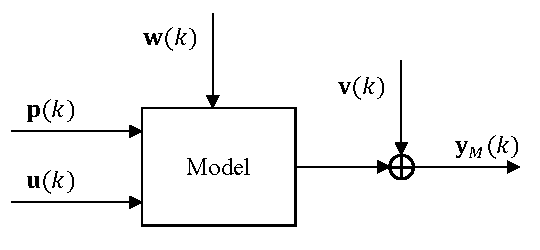
\includegraphics[width=8cm]{images/model_diag_upwvy.pdf}
	\caption{System model with disturbance inputs and manipulated inputs}
	\label{fig:model_diag_upwvy}
\end{figure}
In the case where the system has unmeasured disturbance inputs, $\mathbf{p}(k) \in \mathbb{R}^{n_p}$, as depicted in Figure \ref{fig:model_diag_upwvy}, the state-space equations \eqref{eq:ss_rep_uwy} are modified to include these by splitting the input matrix into two parts, $\mathbf{B}_u \in \mathbb{R}^{n \times n_u}$ and $\mathbf{B}_p \in \mathbb{R}^{n \times n_p}$,
\begin{equation} \label{eq:ss_rep_upwy}
	\begin{aligned}
		\mathbf{x}(k+1) = \mathbf{A} \mathbf{x}(k) + \mathbf{B}_u \mathbf{u}(k) + \mathbf{B}_p \mathbf{p}(k) + \mathbf{w}(k), \\
		\mathbf{y}_M(k) = \mathbf{C} \mathbf{x}(k) + \mathbf{v}(k).
	\end{aligned}
\end{equation}

For state estimation in the presence of unmeasured disturbances, which is always the case in practice, a suitable model of the disturbances is needed. This model is shown in Figure \ref{fig:model_diag_wpupwvy} with a vector of random shock variables, $\mathbf{w}_p(k)$, at its input.
\nomenclature{$\mathbf{w}_p(k)$}{random shock signals at time $k$}%
\begin{figure}[ht]
	\centering
	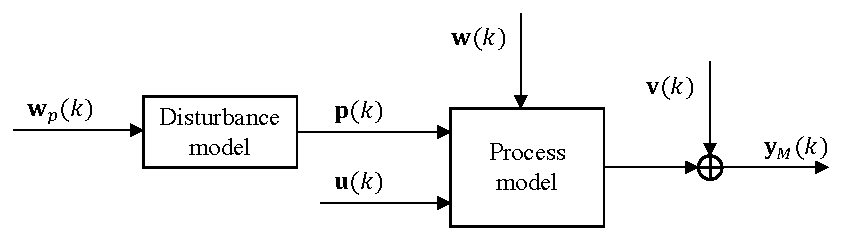
\includegraphics[width=12.5cm]{images/model_diag_wpupwvy.pdf}
	\caption{System with process model and disturbance model}
	\label{fig:model_diag_wpupwvy}
\end{figure}

A state-space representation of the combined system including the disturbance model can be constructed. This is referred to as the \textit{augmented system model},
\begin{equation} \label{eq:ss_rep_xa}
	\begin{aligned}
		\mathbf{x}_a(k+1) = \mathbf{A}_a \mathbf{x}_a(k) + \mathbf{B}_{a,u} \mathbf{u}(k) + \mathbf{B}_{a,w} \mathbf{w}_{a}(k), \\
		\mathbf{y}(k) = \mathbf{C}_a \mathbf{x}_a(k) + \mathbf{v}(k),
	\end{aligned}
\end{equation}
%\nomenclature{$\mathbf{x}_a(k)$}{augmented system states at time $k$}%
where $\mathbf{x}_a(k) \in \mathbb{R}^{n+n_p}$ is an augmented state vector that includes the states of both the process model and the disturbance model, 
\begin{equation} \label{eq:xak}
	\mathbf{x}_a(k) = \begin{bmatrix}
		\mathbf{x}(k) \\
		\mathbf{x}_p(k)
	\end{bmatrix},
\end{equation}
and $\mathbf{w}_a(k) \in \mathbb{R}^{n+n_p}$ is an augmented vector of random variables, including the random shocks,
\begin{equation} \label{eq:wak}
	\mathbf{w}_a(k) = \begin{bmatrix}
		\mathbf{w}(k) \\
		\mathbf{w}_p(k)
	\end{bmatrix}.
\end{equation}

However, note that this notation with subscript `a' is only used in this section. In subsequent sections, the subscript is dropped for simplicity since all references to the system model refer to the augmented model used for state estimation.

Although the random shock in a \gls{RODD} is unmeasured, it may be observable from the measurements of the outputs of the system. As mentioned in Section \ref{detection_RODDs}, systems with \gls{RODD}s pose problems for state estimation using standard Kalman filters due to the switching of the noise model parameters, namely, the variance of $w_p(k)$ \eqref{eq:wpk2}. As explained by \cite{andersson_adaptive_1985}, a trade-off must be made during the filter design between its ability to respond to the infrequent disturbance when it occurs, and its sensitivity to noise at other times.


\subsection{Multiple model approaches} \label{sec:multi-model}

One option for state estimation of switching (i.e. hybrid) systems is the so-called \textit{multiple-model approach}. Multiple-model observers account for different possible hypotheses about the current and past states of the system and infer from these an overall `best' estimate of the current states. To achieve this, an independent Kalman filter is maintained for each hypothesis and a weighted average of the estimates by each filter is calculated using the conditional probabilities of each hypothesis given current and past measurements.

Let the number of hypotheses and Kalman filters be $n_h$ and the \textit{shock mode hypothesis} associated with Kalman filter $f$ at time $k$ be
\nomenclature{$n_h$}{number of hypotheses maintained by a multiple-model observer}%
\begin{equation} \label{eq:gammak}
	\gamma_{f}(k) \in \left\{0, 1 \right\} \forall{k \ge 0}.
\end{equation}

First, consider the case of estimating only one shock signal \eqref{eq:wpk2}. Therefore, $\gamma_f(k)$ is a scalar. The transition probabilities of the random shock are independent of previous shocks:
\nomenclature{$\gamma_f(k)$}{random shock indicator of hypothesis $f$ at time $k$}%
\begin{equation} \label{eq:Pr_gammak_given_gammakm1}
	\begin{aligned}
		& \Pr\left(\gamma_{f}(k)=0 \mid \gamma_{f}(k-1)\right) = \Pr\left(\gamma_{f}(k)=0\right) = 1-\varepsilon, \\
		& \Pr\left(\gamma_{f}(k)=1 \mid \gamma_{f}(k-1)\right) = \Pr\left(\gamma_{f}(k)=1\right) = \varepsilon.
	\end{aligned}
\end{equation}

After $k$ time steps, the complete shock mode hypothesis sequence associated with filter $f$ is
\nomenclature{$\Gamma_f(k)$}{shock indicator hypotheses sequence $f$ from time $0$ to $k$}%
\begin{equation} \label{eq:Gammak}
	\Gamma_f(k) = \left\{ \gamma_f(0), \gamma_f(1), ..., \gamma_f(k) \right\}.
\end{equation}

The known system inputs and output measurements up to time $k$ are
\nomenclature{$\mathbf{U}(k)$}{known system inputs from time 0 to time $k$}%
\nomenclature{$\mathbf{Y}(k)$}{system outputs from time 0 to time $k$}%
\nomenclature{$\mathbf{Y}_M(k)$}{system output measurements from time 0 to time $k$}%
\begin{equation} \label{eq:Uk_Yk}
	\begin{aligned}
		\mathbf{U}(k) = \left\{ \mathbf{u}(0), \mathbf{u}(1), ..., \mathbf{u}(k) \right\} \\
		\mathbf{Y}_M(k) = \left\{ \mathbf{y}_M(0), \mathbf{y}_M(1), ..., \mathbf{y}_M(k) \right\}.
	\end{aligned}
\end{equation}

Assume that new measurements are made available at each time $k$. The probability of the shock hypothesis sequences associated with each filter given the data up to time $k$ can be calculated recursively using the following equations. At time $k$, the probability of the shock hypothesis sequence associated with filter $f$ given the data up to time $k-1$ is
\begin{multline} \label{eq:Pr_Gammak_given_Ykm1}
	\Pr(\Gamma_f(k) \mid \mathbf{Y}_M(k-1)) = 
	\Pr(\gamma_f(k) \mid \gamma_f(k-1)) \Pr(\Gamma_f(k-1) \mid \mathbf{Y}_M(k-1)).
\end{multline}

The conditional probability densities of the measurements, $\mathbf{y}_M(k)$, are approximated by Gaussian distributions centred on the output predictions, $\mathbf{\hat{y}}_{f}(k \mid k-1)$,  and with the variance of the output prediction error, $\mathbf{S}_f(k)$,
\begin{equation} \label{eq:p_yk_given_Gammak_Ykm1}
	p(\mathbf{y}_M(k) \mid \Gamma_f(k), \mathbf{Y}_M(k-1)) \approx \mathcal{N}\left(\mathbf{y}_M(k), \mathbf{\hat{y}}_{f}(k \mid k-1),	\mathbf{S}_f(k) \right)
\end{equation}
\nomenclature{$\mathcal{N}(\mathbf{y}, \mathbf{\mu}, \Sigma)$}{multivariate normal probability density of $\mathbf{y}$ with mean $\mathbf{\mu}$ and covariance $\Sigma$}%
where $p(\cdot)$ here represents a probability density function and $\mathcal{N}(\mathbf{y}, \mathbf{\mu}, \Sigma)$ denotes the multivariate normal probability density of $\mathbf{y}$ with mean $\mathbf{\mu}$ and variance $\Sigma$. $\mathbf{\hat{y}}_{f}(k \mid k-1)$ and $\mathbf{S}_f(k)$ are calculated as $\mathbf{\hat{y}}(k \mid k-1)$ and $\mathbf{S}(k)$ for a single Kalman filter, using 
\begin{equation} \label{eq:yfk_pred}
	\mathbf{\hat{y}}_{f}(k \mid k-1) = \mathbf{C}\mathbf{\hat{x}}_{f}(k \mid k-1)
\end{equation}
and
\nomenclature{$\mathbf{S}_f(k)$}{covariance of the output prediction errors of Kalman filter $f$ at time $k$}%
\begin{equation} \label{eq:Sfk}
	\mathbf{S}_f(k) = \mathbf{C}\mathbf{P}_f(k \mid k-1)\mathbf{C}^\intercal + \mathbf{R},
\end{equation}
where $\mathbf{\hat{x}}_{f}(k \mid k-1)$ and $\mathbf{P}_f(k \mid k-1)$ are the state predictions and prediction error covariances of Kalman filter $f$ calculated in the previous time step.

Finally, the estimate of the probability of shock hypothesis sequence $\Gamma_f(k)$ given the data up to time $k$ is
\begin{equation} \label{eq:Pr_Gammak_given_Yk}
	\Pr(\Gamma_f(k) \mid \mathbf{Y}_M(k)) = \frac{q_f(k)}{\sum_{f=1}^{n_h} q_f(k)},
\end{equation}
where
\begin{equation} \label{eq:qfk}
	q_f(k) = p(\mathbf{y}_M(k) \mid \Gamma_f(k), \mathbf{Y}_M(k-1)) \Pr(\Gamma_f(k) \mid \mathbf{Y}_M(k-1)).
\end{equation}

The Kalman filters for tracking each hypothesis use the state-space representation of the augmented system model \eqref{eq:ss_rep_xa}. Since the system includes a \gls{RODD} with a switching noise variance, it is a \textit{hybrid dynamical system} (refer to Section \ref{sec:lit-hybrid}). Define the set of possible covariance matrices of this system as
\begin{equation} \label{eq:init_Q_R}
	\mathcal{Q} = \left\{\mathbf{Q}_0, \mathbf{Q}_1\right\},
\end{equation}
and, for convenient notation, let $\mathcal{Q}$ be indexed by the shock indicator $\gamma_f(k)$,
\begin{equation} \label{eq:init_Q}
	\mathcal{Q}(\gamma_f(k)) = 
	\begin{cases*}
		\mathbf{Q}_0 & \text{if} $\gamma_f(k)=0$, \\
		\mathbf{Q}_1 & \text{if} $\gamma_f(k)=1$.
	\end{cases*}
\end{equation}

At the start of a simulation, $f$ Kalman filters are initialized with initial state estimates, $\mathbf{\hat{x}}_f(0) = \mathbf{\hat{x}}_{f,0}$, and initial error covariance estimates $	\mathbf{P}_f(0) = \mathbf{P}_{f,0}$. At each time instant, starting at $k=0$, the correction gains are calculated as in the previous section \eqref{eq:Kk},
\nomenclature{$\mathbf{K}_f(k)$}{correction gain (filtering form) of Kalman filter $f$}%
\begin{equation} \label{eq:Kfk}
	\mathbf{K}_f(k) = \mathbf{P}_f(k \mid k-1)\mathbf{C}^\intercal \mathbf{S}_f^{-1}(k).
\end{equation}

The corrected state and output estimates are calculated as in \eqref{eq:xkyk_hat}, given the current measurement using
\nomenclature{$\mathbf{\hat{x}}_f(k \mid k)$}{estimates of the system states at time $k$ for hypothesis $f$}%
\nomenclature{$\mathbf{\hat{y}}_f(k \mid k)$}{estimates of the system outputs at time $k$ for hypothesis $f$}%
\begin{equation} \label{eq:xfkyfk_hat}
	\begin{aligned}
		\mathbf{\hat{x}}_f(k \mid k) &= \mathbf{\hat{x}}_f(k \mid k-1) + \mathbf{K}_f(k) \big( \mathbf{y}_M(k) - \mathbf{C} \mathbf{\hat{x}}_f(k \mid k-1) \big) \\
		\mathbf{\hat{y}}_f(k \mid k) &= \mathbf{C} \mathbf{\hat{x}}_f(k \mid k).
	\end{aligned}
\end{equation}

The corrected error covariances are calculated as in \eqref{eq:Pk-stab} using 
\nomenclature{$\mathbf{P}_f(k \mid k)$}{state estimation error covariance of filter $f$ at time $k$ made with information available at time $k$}%
\nomenclature{$\mathbf{P}_f(k \mid k-1)$}{predictions of the state estimation error covariance of filter $f$ at time $k$ made with information available at time $k-1$}%
\begin{equation} \label{eq:Pkf-stab}
	\mathbf{P}_f(k \mid k) = \left( \mathbf{I}_n - \mathbf{K}_f(k) \mathbf{C} \right ) \mathbf{P}_f(k \mid k-1) \left( \mathbf{I}_n - \mathbf{K}_f(k) \mathbf{C} \right )^\intercal + \mathbf{K}_f(k) \mathbf{R} \mathbf{K}_f(k)^\intercal.
\end{equation}

An additional precaution is necessary here for numerical stability. $\mathbf{P}_f(k \mid k)$ should always be positive definite. However, because finite floating-point representations are inexact, it may potentially loose its positive definiteness. If this occurs, then $\mathbf{S}_f(k)$ will also not be positive definite, and a numerical error is likely when calculating the probability density of the output estimates \eqref{eq:p_yk_given_Gammak_Ykm1}. To avoid this problem the following operation is carried out after \eqref{eq:Pkf-stab}
\begin{equation} \label{eq:Pkf-psd-fix}
	\mathbf{P}_f(k \mid k) \gets \frac{ \mathbf{P}_f(k \mid k) + \mathbf{P}_f(k \mid k)^\intercal )}{2}. 
\end{equation}

This ensures that $\mathbf{P}_f(k \mid k)$ is always positive definite.

The predicted states at the next time instant are calculated as in \eqref{eq:xkp1_hat}
\begin{equation} \label{eq:xfkp1_hat}
	\mathbf{\hat{x}}_f(k+1 \mid k) = \mathbf{A} \mathbf{\hat{x}}_f(k \mid k) + \mathbf{B} \mathbf{u}(k)
\end{equation}
and the predicted error covariances at the next time instant are calculated as in \eqref{eq:Pkp1} using
\nomenclature{$\mathbf{P}_f(k+1 \mid k)$}{predictions of the state estimation error covariance of filter $f$ at time $k+1$ made with information available at time $k$}%
\begin{equation} \label{eq:Pfkp1}
	\mathbf{P}_f(k+1 \mid k) = \mathbf{A} \mathbf{P}_f(k \mid k)  \mathbf{A}^\intercal  + \mathcal{Q}(\gamma_f(k)).
\end{equation}

Note the difference between \eqref{eq:Pfkp1} and \eqref{eq:Pkp1}.  Here, $\mathbf{P}_f(k+1 \mid k)$ is dependent on $\gamma_f(k)$, which determines the noise covariance matrix used in the update, whereas in \eqref{eq:Pkp1}, $\mathbf{Q}$ is time invariant.

Finally, the merged estimates of the states and outputs at the current time are the sum of the Kalman filter estimates weighted by the conditional probabilities from \eqref{eq:Pr_Gammak_given_Yk},
\begin{equation} \label{eq:xkyk_hat_MKF}
	\begin{aligned}
		\mathbf{\hat{x}}(k \mid k) = \sum_{f=1}^{n_h} \mathbf{\hat{x}}_f(k \mid k) \Pr(\Gamma_f(k) \mid \mathbf{Y}_M(k)) \\
		\mathbf{\hat{y}}(k \mid k) = \sum_{f=1}^{n_h} \mathbf{\hat{y}}_f(k \mid k) \Pr(\Gamma_f(k) \mid \mathbf{Y}_M(k)).
	\end{aligned}
\end{equation}

A merged estimate of the covariance of the estimation errors is obtained using
\begin{equation} \label{eq:Pk_MKF}
	\begin{aligned}
	\mathbf{P}(k \mid k) = \sum_{f=1}^{n_h} \Pr(\Gamma_f(k) \mid \mathbf{Y}_M(k)) \left( \mathbf{P}_f(k \mid k) + \delta_\mathbf{\hat{x}}(k) \delta_\mathbf{\hat{x}}^\intercal(k) \right), \\
	\delta_\mathbf{\hat{x}}(k) = \mathbf{\hat{x}}(k \mid k) - \mathbf{\hat{x}}_f(k \mid k).
	\end{aligned}
\end{equation}

Algorithm \ref{alg:afmm} shows the sequence of operations and flow control loops to execute these computations during a simulation of length $N$ time steps.
\nomenclature{$N$}{length of a simulation in number of sampling intervals}%
\begin{algorithm}
	\caption{Multiple model observer simulation}  \label{alg:afmm}
	%\algorithmfootnote{$y_0$ denotes the initial value.}
	\begin{algorithmic}
			\Require $\mathbf{A}, \mathbf{B}, \mathbf{C}, \mathbf{\hat{x}}_0, \mathbf{\gamma}_{\text{init}}, \mathbf{p}_{\text{init}}, \mathbf{P}_0, \mathcal{Q}, \mathbf{R}, \Pi, \mathbf{U}(N), \mathbf{Y}_M(N)$
			\For{$f \gets 1, n_h$}  \Comment{Initialize Kalman filters}  % \footnotemark
				\State $\mathbf{\hat{x}}_f(0 \mid -1) \gets \mathbf{\hat{x}}_0$
				\State $\mathbf{P}_f(0 \mid -1) \gets \mathbf{P}_0$
				\State $\mathbf{\gamma}_f(-1) \gets \mathbf{\gamma}_{\text{init},f}$
				\State $\Pr(\Gamma_f(-1)|\mathbf{Y}_M(-1))) \gets p_{\text{init},f}$
			\EndFor
			\For{$k \gets 0, N$}
			\For{$f \gets 1, n_h$}
				\State calculate $\mathbf{\hat{y}}_f(k \mid k-1)$ \eqref{eq:yfk_pred} \Comment{KF output predictions}
				\State calculate $\mathbf{S}_f(k \mid k-1)$ \eqref{eq:Sfk}
			\EndFor
			\State $\mathbf{y}_M(k) \gets \mathbf{Y}_M(k)$ \Comment{Acquire measurements}  % \footnotemark
			\State $\mathbf{u}(k) \gets \mathbf{U}(k)$
			\For{$f \gets 1, n_h$}
				\State calculate $\Pr(\Gamma_f(k) \mid \mathbf{Y}_M(k))$ (\ref{eq:Pr_Gammak_given_Ykm1}, \ref{eq:p_yk_given_Gammak_Ykm1}, \ref{eq:Pr_Gammak_given_Yk}, \ref{eq:qfk})     \Comment{Probability update}  % \footnotemark
			\EndFor
			\State $\Gamma_f(k \mid k), \mathbf{\hat{x}}_f(k \mid k), \mathbf{P}_f(k \mid k) \gets ...$ \Comment{branching, pruning, and merging procedures}  % \footnotemark
			\For{$f \gets 1, n_h$}
				\State calculate $\mathbf{K}_f(k)$ \eqref{eq:Kfk} \Comment{KF updates}
				\State calculate $\mathbf{\hat{x}}_f(k \mid k), \mathbf{\hat{y}}_f(k \mid k)$ \eqref{eq:xfkyfk_hat}
				\State calculate $\mathbf{P}_f(k \mid k)$ \eqref{eq:Pkf-stab}
			\EndFor
			\State calculate $\mathbf{\hat{x}}(k \mid k), \mathbf{\hat{y}}(k \mid k)$ \eqref{eq:xkyk_hat} \Comment{States and output estimate}
			\State calculate $\mathbf{P}(k \mid k)$ \eqref{eq:Pk_MKF} \Comment{Error covariance}  % \footnotemark
			\For{$f \gets 1, n_h$}
				\State calculate $\mathbf{\hat{x}}_f(k+1 \mid k)$ \eqref{eq:xfkp1_hat} \Comment{KF state predictions}
				\State calculate $\mathbf{P}_f(k+1 \mid k)$ \eqref{eq:Pfkp1}
			\EndFor
			\EndFor
		\end{algorithmic}
\end{algorithm}

% Version with footnotes - not working
%\begin{algorithm}
%	\caption{Multiple model observer calculations} \label{alg:afmm}
%	%\algorithmfootnote{$y_0$ denotes the initial value.}
%	\begin{algorithmic}
%		\Require $\mathbf{A},\mathbf{B},\mathbf{C},\mathbf{\hat{x}}(0), \mathbf{P}(0), \mathcal{Q}, \mathbf{R}, \varepsilon, \mathbf{U}(N), \mathbf{Y}_M(N)$
%		\State $\mathbf{\hat{x}}_1(0) \gets \mathbf{\hat{x}}(0)$  \Comment{Initialize Kalman filters\footnotemark}
%		\State $\mathbf{P}_1(0) \gets \mathbf{P}(0)$
%		\State $\Pr(\Gamma_1(k-1)|\mathbf{Y}_M(k-1))) \gets 1$
%		\For{$f \gets 2, n_h$}
%		\State $\mathbf{\hat{x}}_f(0) \gets \mathbf{\hat{x}}(0)$
%		\State $\mathbf{P}_f(0) \gets 10^{10}\mathbf{P}(0)$
%		\State $\Pr(\Gamma_f(k-1)|\mathbf{Y}_M(k-1))) \gets 1^{-10}$
%		\EndFor
%		\For{$k \gets 0, N$}
%		\State $\Gamma_f(k), \mathbf{\hat{x}}_f(k), \mathbf{P}_f(k) \gets ...$ \Comment{Sub-optimal procedure occurs here\footnotemark}
%		\For{$f \gets 1, n_h$}
%		\State calculate $\Pr(\Gamma_f(k) \mid \mathbf{Y}_M(k))$ (\ref{eq:Pr_Gammak_given_Ykm1}, \ref{eq:p_yk_given_Gammak_Ykm1}, \ref{eq:Pr_Gammak_given_Yk}, \ref{eq:qfk})
%		\State calculate $\mathbf{K}_f(k)$ \eqref{eq:Kf} \Comment{Filter updates}
%		\State calculate $\mathbf{\hat{x}}_f(k+1 \mid k)$ \eqref{eq:xfkp1_hat}
%		\State update $\mathbf{P}_f(k+1 \mid k)$ \eqref{eq:Pfk}
%		\EndFor
%		\State calculate $\mathbf{\hat{x}}(k+1 \mid k)$ \eqref{eq:xkyk_hat} \Comment{State estimate}
%		\State calculate $\mathbf{P}(k+1 \mid k)$ \Comment{Error covariance\footnotemark}
%		\EndFor
%	\end{algorithmic}
%\end{algorithm}
%
%\addtocounter{footnote}{-3} %3=n
%\stepcounter{footnote}\footnotetext{To initialize the bank of $n_h$ Kalman filters, initialize one with an available estimate and covariance of the initial state of the system and set the covariances of all others to high values to ensure they are eliminated as soon as better estimates are available.}
%\stepcounter{footnote}\footnotetext{At this point, the algorithm must extend the shock indicator sequences to the current time instant, while limiting the total number of hypotheses and filters according to a particular sub-optimal method such as the procedures described in section \ref{sec:pruning} and \ref{sec:fusion}.
%\stepcounter{footnote}\footnotetext{The estimation error covariance is not required by the algorithm. It may be calculated if needed.}

The multiple-model observer concept can be used for state estimation of any MJLS \eqref{eq:MJLS} with switching $\mathbf{A}$, $\mathbf{B}$, $\mathbf{C}$, $\mathbf{D}$, $\mathbf{w}_p(k)$, or $\mathbf{e}_p(k)$. However, the number of independently-switching components is severely limited in practice due to the number of hypotheses that would need to be simulated.

\subsection{Sub-optimal algorithms} \label{sec:sub-opt}

The problem that sub-optimal algorithms address is the inevitable growth in the number of hypotheses that would have to be modelled in an optimal multiple-model observer. For a system with one \gls{RODD} disturbance, the number of possible hypotheses doubles each time step because each current hypothesis branches into two—one corresponding to the assumption of no shock in the next time period and the other to that of a shock. Figure \ref{fig:mm-obs-br} illustrates that after 3 time instants starting at $k=0$, eight hypotheses are needed to represent the possible shock sequences. For a system with two independent \gls{RODD} disturbances, the number would be 64.

\begin{figure}[ht]
	\centering
	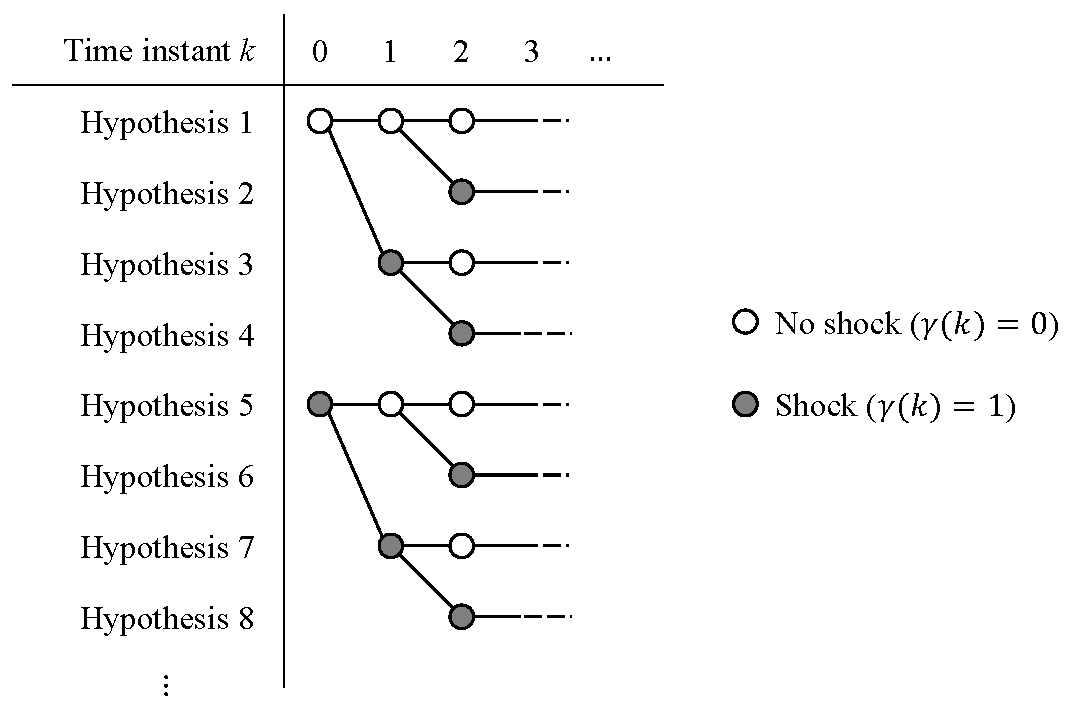
\includegraphics[height=7.5cm]{images/mm_obs_seq_br.pdf}
	\caption{Sequence branching}
	\label{fig:mm-obs-br}
\end{figure}

\subsubsection{Generalised pseudo-Bayes algorithm} \label{sec:GPB}

One of the simplest sub-optimal multiple-model methods is the \textit{generalised pseudo-Bayesian algorithm} \citep{buxbaum_recursive_1969, jaffer_estimation_1971, tugnait_detection_1982}. Although not used directly in this work, the method is described here because it is a starting point for understanding hypotheses branching and merging, which are techniques used in the sequence fusion algorithm described by \cite{robertson_detection_1995}.

There are two basic versions of the algorithm, the \acrlong{GPB1} (\acrshort{GPB1}), and the \acrlong{GPB2} (\acrshort{GPB2}). Figure \ref{fig:mm-obs-gpb1} shows a simplified diagram of the \gls{GPB1} process in the case of a system with two modes ($n_j=2$). A single estimate of the system states and error covariance at time $k$ is branched into $n_j$ hypotheses representing the possible modes of the system at that time. In this context, \textit{branching} simply means duplicating or cloning the hypothesis state estimates and error covariance into $n_j$ copies. These are then used to initialise $n_j$ Kalman filters. Each Kalman filter then makes a prediction of the states in the next time instant using the system model associated with one of the possible modes. In the next time instant, the $n_j$ predictions are corrected using the measurements, and the updated estimates are merged into a single set of estimates using the multiple-model observer merging procedure defined by (\ref{eq:xkyk_hat_MKF}, \ref{eq:Pk_MKF}). These branching and merging steps are then repeated at each subsequent time step.
\begin{figure}[ht]
	\centering
	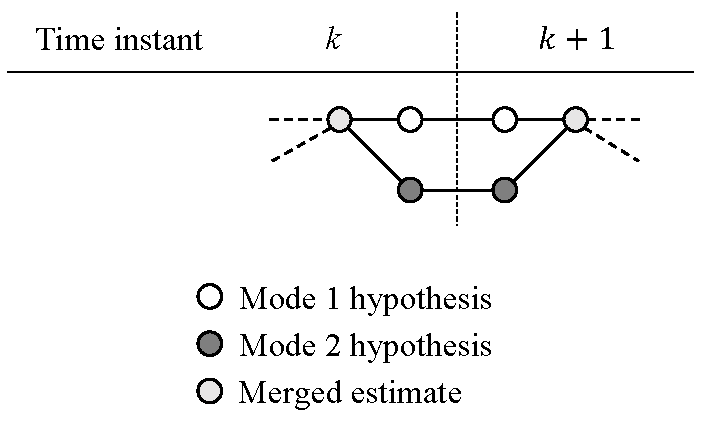
\includegraphics[height=5cm]{images/mm_obs_seq_gpb1.pdf}
	\caption{Simplified diagram of the \gls{GPB1} algorithm ($n_j=2$)}
	\label{fig:mm-obs-gpb1}
\end{figure}

Whereas the \gls{GPB1} estimator considers $n_j$ possible mode transitions from time $k-1$ to time $k$, the \gls{GPB2} estimator considers $n_j^2$ possible transition sequences from time $k-2$ to time $k$. Figure \ref{fig:mm-obs-gpb2} shows a simplified diagram of the \gls{GPB2} algorithm in the case of two system modes ($n_j=2$). At time $k$ it maintains $n_j$ merged estimates and associated variables, $\left\{ \hat{\mathbf{x}}_m(k \mid k), \mathbf{P}_m(k \mid k), \hat{\mathbf{y}}_m(k \mid k), \Pr(\Gamma_m(k) \mid \mathbf{Y}_M(k)) \right\}$, for $m=1,2,...,n_j$. Each of these is then branched into $n_j$ estimates, creating a total of $n_h=n_j^2$ hypotheses, represented by $n_h$ Kalman filters labelled $f=1,2,...n_h$. At time $k+1$, the Kalman filter predictions are corrected to produce $n_h$ estimates. Then, two merging operations are carried out on these estimates. The first merges the $n_h$ estimates into $n_m=n_j$ estimates for use in the next step. The second merges the $n_m$ merged estimates again, into one final estimate which is the output of the observer and is not used in subsequent steps.
\begin{figure}[ht]
	\centering
	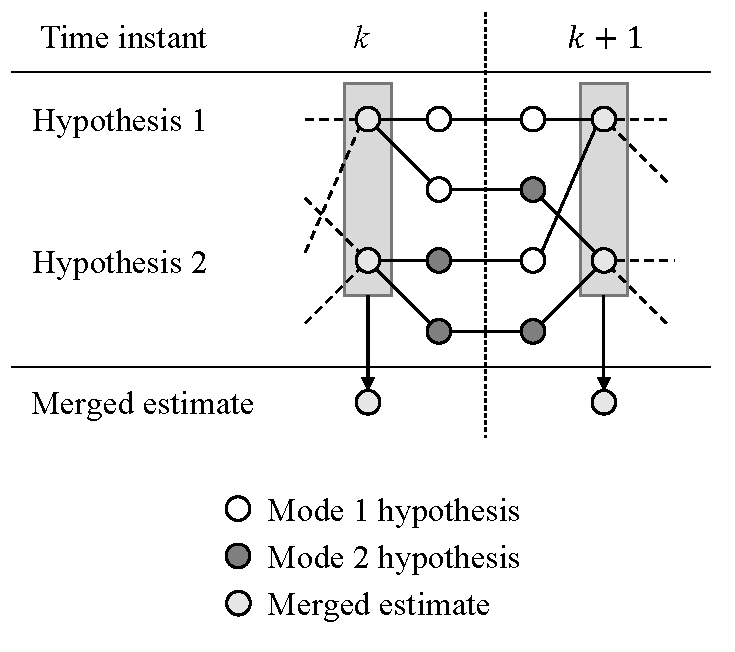
\includegraphics[height=6.5cm]{images/gpb2_diagram.pdf}
	\caption{Simplified diagram of the \gls{GPB2} algorithm ($n_j=2$)}
	\label{fig:mm-obs-gpb2}
\end{figure}

The $n_m$ merged estimates and covariances at time $k$ are produced by calculating weighted sums of the estimates and covariances of the branched hypotheses,
\nomenclature{$n_m$}{number of merged hypotheses maintained by a multiple-model observer}%
\nomenclature{$\mathbf{\hat{x}}_m(k \mid k)$}{merged estimates of the system states at time $k$ for merged hypothesis $m$}%
\nomenclature{$\mathbf{\hat{y}}_m(k \mid k)$}{merged estimates of the system outputs at time $k$ for merged hypothesis $m$}%
\nomenclature{$\mathbf{P}_m(k \mid k)$}{merged state estimation error covariance at time $k$ for merged hypothesis $m$}%
\nomenclature{$\Gamma_m(k)$}{merged shock hypothesis $m$ at time $k$}%
\begin{equation} \label{eq:xmkymk_hat_MKF}
	\begin{aligned}
		\mathbf{\hat{x}}_m(k \mid k) = \frac{1}{Z_m(k)} \sum_{f \in \mathcal{H}_{\text{merge},m}} \mathbf{\hat{x}}_f(k \mid k) \Pr(\Gamma_f(k) \mid \mathbf{Y}_M(k)), \\
		\mathbf{\hat{y}}_m(k \mid k) = \frac{1}{Z_m(k)} \sum_{f \in \mathcal{H}_{\text{merge},m}} \mathbf{\hat{y}}_f(k \mid k) \Pr(\Gamma_f(k) \mid \mathbf{Y}_M(k)),\\
		\mathbf{P}_m(k \mid k) = \frac{1}{Z_m(k)} \sum_{f \in \mathcal{H}_{\text{merge},m}} \Pr(\Gamma_f(k) \mid \mathbf{Y}_M(k)) \left( \mathbf{P}_f(k \mid k) + \delta_\mathbf{\hat{x}}(k) \delta_\mathbf{\hat{x}}^\intercal(k) \right), \\
		\delta_\mathbf{\hat{x}}(k) = \mathbf{\hat{x}}_m(k \mid k) - \mathbf{\hat{x}}_f(k \mid k), \\
		\Pr(\Gamma_m(k) \mid \mathbf{Y}_M(k)) = \sum_{f \in \mathcal{H}_{\text{merge},m}} \Pr(\Gamma_f(k) \mid \mathbf{Y}_M(k)).
	\end{aligned}
\end{equation}
\nomenclature{$\mathcal{H}_{\text{merge}}$}{hypothesis index used in merging operations}%
where $\mathcal{H}_{\text{merge}}$ is a set of $n_m$ indices that determine which hypotheses are merged to produce each merged estimate, and $Z_m(k)$ is a scalar normalization variable given by
\nomenclature{$Z_m(k)$}{normalization variable at time $k$ used in merged probability calculations}%
\begin{equation} \label{eq:Zmk}
	Z_m(k) = \sum_{f \in \mathcal{H}_{\text{merge},m}} \Pr(\Gamma_f(k) \mid \mathbf{Y}_M(k)).
\end{equation}

In the case of \gls{GPB2}, $\mathcal{H}_{\text{merge}}$ is defined
\begin{equation} \label{eq:Hmerge_GPB2}
	\mathcal{H}_{\text{merge}} = \begin{Bmatrix} \mathcal{H}_{\text{merge},1} \\ \mathcal{H}_{\text{merge},2} \end{Bmatrix} = \begin{Bmatrix}
		\begin{bmatrix}	1 \\ 3 \end{bmatrix} \\
		\begin{bmatrix}	2 \\ 4 \end{bmatrix}
	\end{Bmatrix}.
\end{equation}
This means that merged estimate $\mathbf{\hat{x}}_1(k \mid k)$ is calculated by merging the estimates associated with branched hypotheses 1 and 3, and merged estimate $\mathbf{\hat{x}}_2(k \mid k)$ is calculated by merging the estimates of branched hypotheses 2 and 4.

An associated index, $\mathcal{H}_{\text{branch}}$, governs the branching operation, which for \gls{GPB2} is
\nomenclature{$\mathcal{H}_{\text{branch}}$}{hypothesis index used in branching operations}%
\begin{equation} \label{eq:Hbranch_GPB2}
	\mathcal{H}_{\text{branch}} = \begin{bmatrix} 1 \\ 1 \\ 2 \\ 2 \end{bmatrix}.
\end{equation}
This indicates that branched estimates 1 and 2 are clones of merged estimate $\mathbf{\hat{x}}_1(k \mid k)$ and branched estimates 3 and 4 are clones of merged estimate $\mathbf{\hat{x}}_2(k \mid k)$. These definitions match the branching and merging operations depicted in Figure \ref{fig:mm-obs-gpb2}.

% TODO: We don't need this if we define the r(k) and r_m(k) transitions.
The system modes, which determine the system model parameters as well as the mode transition probabilities, evolve according to the branching and merging indices. Starting with the modes associated with the merged hypotheses at time $k$, which in the case of GPB2 are
\nomenclature{$\mathbf{r}_m(k)$}{indicators of the system modes of the merged hypotheses at time $k$ used in branching and merging operations}%
\begin{equation} \label{eq:rmk_GPB2}
		\mathbf{r}_m(k) = \begin{bmatrix} 1 \\ 2 \end{bmatrix},
\end{equation}
the branched modes after branching at time $k$ and before merging at time $k+1$ are
\nomenclature{$\mathbf{r}_{b,1}(k)$}{indicators of the system modes of the branched hypotheses at time $k$ before merging}%
\nomenclature{$\mathbf{r}_{b,2}(k)$}{indicators of the system modes of the branched hypotheses at time $k$ after branching}%
\begin{equation} \label{eq:rbk_GPB2}
	\begin{aligned}
		\mathbf{r}_{b,2}(k) &= \begin{bmatrix} 1 \\ 1 \\ 2 \\ 2 \end{bmatrix},
		\mathbf{r}_{b,1}(k+1) &= \begin{bmatrix} 1 \\ 2 \\ 1 \\ 2 \end{bmatrix}.
	\end{aligned}
\end{equation}
Note that $\mathbf{r}_{b,2}(k)$ is derived by branching $\mathbf{r}_m(k)$ using $\mathcal{H}_{\text{branch}}$ and that when $\mathbf{r}_{b,1}(k+1)$ is merged using $\mathcal{H}_{\text{merge}}$ in the next time step, it leads to 
\begin{equation} \label{eq:rmkp1rmk_GPB2}
	\mathbf{r}_m(k+1) = \begin{bmatrix} 1 \\ 2 \end{bmatrix} = \mathbf{r}_m(k).
\end{equation}
Due to this condition, the algorithm is consistent when executed consecutively every time step.

The advantages of the \gls{GPB1} and \gls{GPB2} estimators are their simplicity, the fact that they can be applied to any switching system, and that the number of hypotheses ($n_j$ or $n_j^2$) is finite and constant, which limits computational requirements. The disadvantages include the fact that they model every possible transition over one or two time steps and merge these into a reduced set of estimates before the next iteration. 

While the branching, modes, and merging steps of the \gls{GPB1} and \gls{GPB2} algorithms are the same each time step, they may be time-varying in the case of the sub-optimal multiple-model algorithms considered in this work. The notation above is easily extended to more complex algorithms with arbitrary branching and merging steps by allowing $\mathcal{H}_{\text{branch}}$, $\mathcal{H}_{\text{merge}}$, $\mathbf{r}_{b,1}(k)$, and $\mathbf{r}_{b,2}(k)$ to be time-varying and by allowing an arbitrarily large number of branched and merged hypotheses, $n_h$ and $n_m$, to exist at each time instant.

\subsubsection{Sequence fusion} \label{sec:fusion}

\cite{robertson_detection_1995} proposed a sub-optimal approach that combines three approximation techniques specifically intended for \gls{RODD} state estimation. The first is referred to as \textit{sequence fusion}. This is based on the assumption that only recent differences in the hypothesis sequences are important for state estimation. Therefore, sequences that are identical over the previous $N_f$ sample times may be merged, where $N_f$ is known as the \textit{fusion horizon}.
\nomenclature{$N_f$}{sequence fusion parameter: length of fusion horizon in number of sampling intervals}%
%The same techniques used in the generalized pseudo-Bayes algorithm are used to perform the sequence branching and merging at each time step. The differences are that more than $n_j^2$ hypotheses are maintained and these are based on longer, pre-specified sequences of possible shocks.

Rather than allowing the number and length of the shock indicator hypothesis sequences, $\Gamma_f(k)$, to grow indefinitely, a fixed number of sequences of length $N_f$ sample periods are defined, each consisting of only the current and the previous $N_f-1$ values of \hl{$\gamma(k)$}
\nomenclature{$\Gamma_m(k-N_f+1,k)$}{merged shock hypotheses $m$ at time $k$ for the fusion horizon $N_f$}%
\begin{equation} \label{eq:Gamma_kmf_k}
	\Gamma_m(k-N_f+1,k) = \{\gamma_m(k-N_f+1), ...,  \gamma_m(k-1), \gamma_m(k)\}, m=1,2,..., n_m.
\end{equation}
These fixed-length sequences are used to merge similar hypotheses so that the total number, $n_m$, remains the same from one time instant to the next.

Secondly, they assume that the exact timing of random shocks is not important and define \textit{detection intervals} of more than one sample period during which it is assumed that only one shock may occur. This is based on the observation that when the correction gain of a Kalman filter increases due to the assumption of a shock occurrence ($\gamma_m(k)=1$), it tends to remain large for several sample periods. The probability of at least one random shock during a detection interval of length $d$ samples is therefore higher than the probability, $\varepsilon$, of a single shock in one sample period, and is given by
\nomenclature{$d$}{sequence fusion parameter: shock spacing or length of detection interval, in number of sampling intervals}
\nomenclature{$\varepsilon_d$}{sequence fusion parameter: probability of at least one shock within the detection interval}%
\begin{equation}  \label{eq:p_gamma_d}
	\varepsilon_d = 1 - (1 - \varepsilon)^{d}.
\end{equation}

The occurrence of one or more shocks within a detection interval is then represented by a single shock at the start of the detection interval and the probabilities of a shock at any other time are set to zero,
\begin{equation} \label{eq:Pr_gamma_nd}
	\begin{aligned}
		\Pr\left(\gamma_{f}(k)=0\right) = \begin{cases*}
			1 - \varepsilon_d & \text { for } $k = d, 2d, 3d, \ldots$ \\
			1 & \text { for } $k \ne d, 2d, 3d, \ldots$
		\end{cases*} \\
		\Pr\left(\gamma_{f}(k)=1\right) = \begin{cases*}
			\varepsilon_d & \text { for } $k = d, 2d, 3d, \ldots$ \\
			0 & \text { for } $k \ne d, 2d, 3d, \ldots$
		\end{cases*} \\
	\end{aligned}
\end{equation}

Thirdly, they rely on the fact that the random shocks occur infrequently and therefore the probability of more than $n_\text{max}$ shocks during the fusion horizon is low, where $n_\text{max}$ may be 1 or some other low number. This further reduces the number of possible hypotheses that must be modelled.
\nomenclature{$n_\text{max}$}{sequence fusion parameter: maximum number of shock occurrences within the fusion horizon}%

To illustrate the resulting shock hypothesis sequences, consider an example. Suppose there is one \gls{RODD} to estimate. A sequence fusion algorithm is used with a fusion horizon of $N_f=9$, a detection interval of $d=3$, and a maximum number of shocks over the fusion horizon of $n_\text{max}=1$. Figure \ref{fig:mm-obs-seq-SFex1} shows the four shock hypotheses that would be required in this case. Note that hypothesis 1 assumes no shocks at any time. Hypothesis 2 assumes shocks occur at times $k=0,9,18,...$. Hypothesis 3 assumes shocks occur at times $k=3,12,21,...$, and so on. After $N_f=9$ sample periods, the sequences repeat indefinitely.

\begin{figure}[ht]
	\centering
	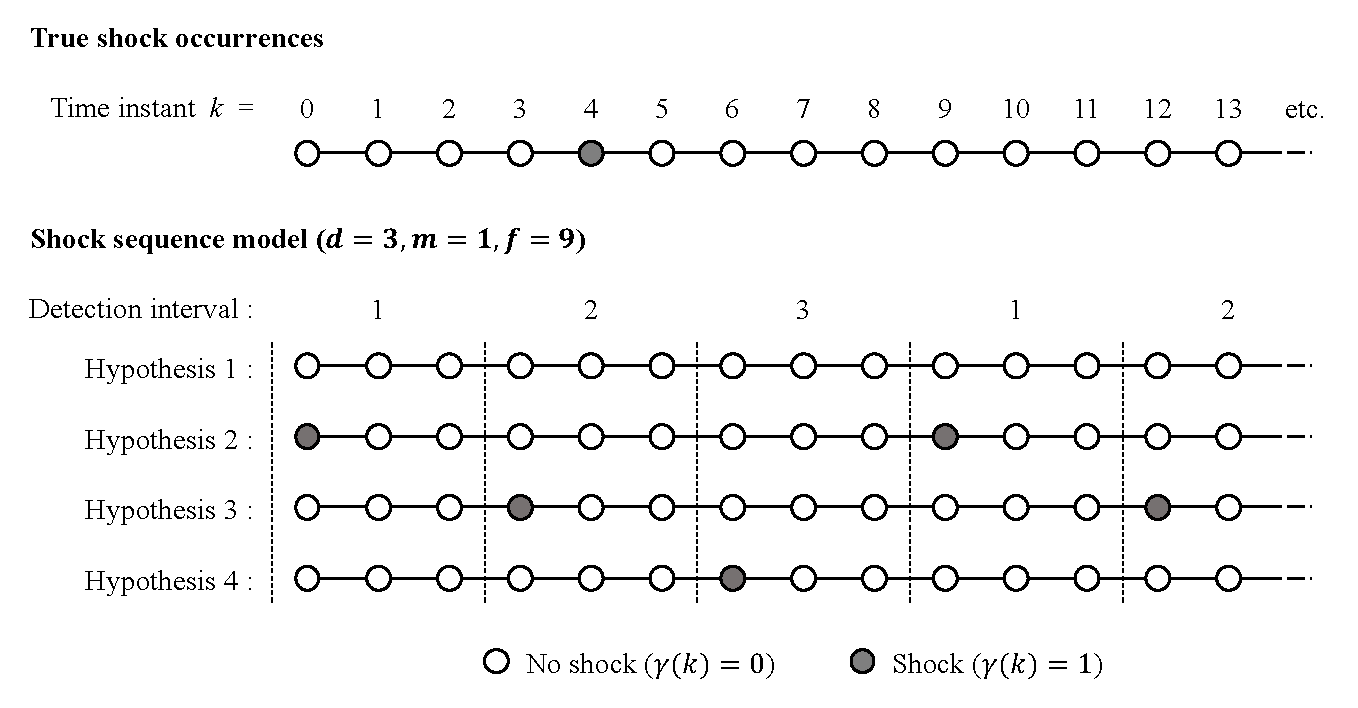
\includegraphics[width=13.5cm]{images/mm_obs_seq_rob1.pdf}
	\caption{Sequence fusion example 1 ($N_f=9$, $n_\text{max}=1$, $d=3$)}
	\label{fig:mm-obs-seq-SFex1}
\end{figure}

Suppose that a shock actually occurred in the system at time $k=4$. In this case, the algorithm should predict that hypothesis 3 is the most likely because this assumes a shock occurred at $k=3$, which is the closest to the actual time.

Figure \ref{fig:mm-obs-seq-SFex2} illustrates a second example with $N_f=10$, $n_\text{max}=2$, and $d=5$. This also has four hypotheses. However, note that hypothesis 4 accounts for the possibility of two shocks within the fusion horizon. As in the previous example, if a true shock occurred at time $k=4$, the most likely hypothesis should be hypothesis 3 because it assumes a shock occurred at $k=5$, which is close to the actual time.
\begin{figure}[ht]
	\centering
	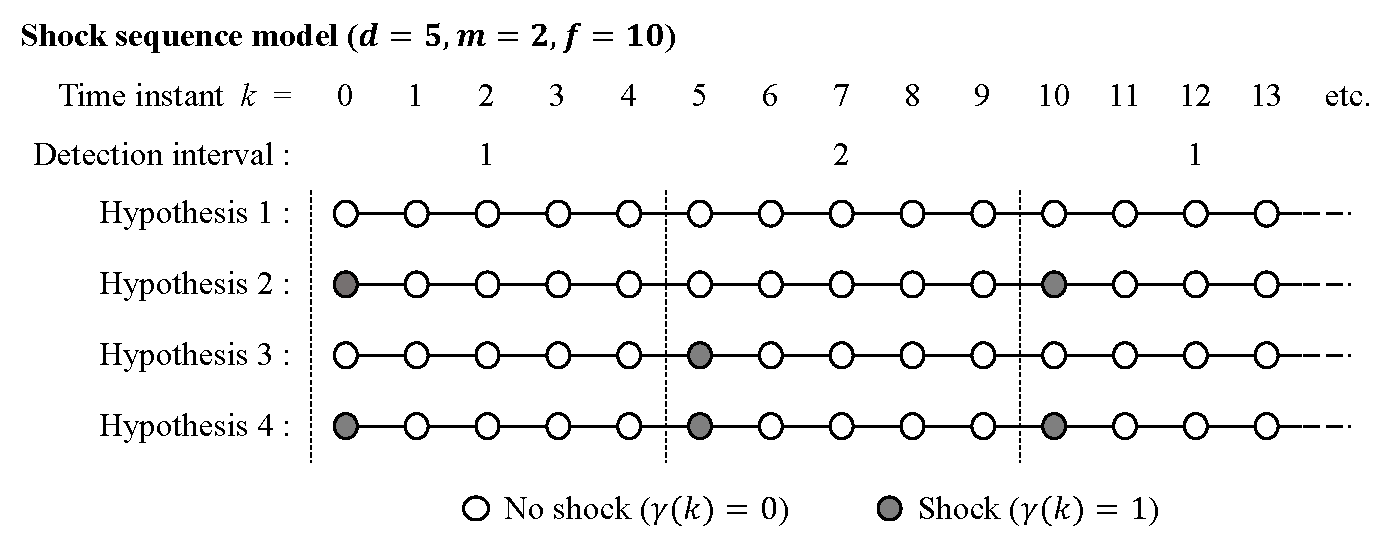
\includegraphics[width=13.5cm]{images/mm_obs_seq_rob2.pdf}
	\caption{Sequence fusion example 2 ($N_f=10$, $n_\text{max}=2$, $d=5$)}
	\label{fig:mm-obs-seq-SFex2}
\end{figure}

As mentioned, the shock hypothesis sequences over the fusion horizon, $\Gamma_m(k-N_f+1,k)$, determine the branching and merging operations that occur at each time step. The logic is as follows: (i) at time $k$, branch each hypothesis sequence into the possible mode transitions that occur between time $k$ and $k+1$, (ii) advance the branched sequences into the next time step, according to the possible mode transitions, (iii) compare the branched sequences and merge those that are identical over the new fusion horizon from time $k-N_f+2$ to $k+1$.

Consider again the sequences from the previous example in Figure \ref{fig:mm-obs-seq-SFex2}. By applying the logic described above, the branching and merging operations depicted in Figure \ref{fig:mm-obs-seq-sf95} may be deduced. For example, consider what happens at time $k=9$. At this time, the fusion horizon spans from time 0 to 9. The four sequences are branched into eight and advanced to the next time instant according to the possible modes at that time (no shock, shock). Then, at time $k=10$ the 8 branched hypotheses are merged back to 4 by combining sequences that are identical over the new fusion horizon, which spans from $k=1$ to 10. Applying this logic each time step, branching and merging are only required once every 5 time steps when shocks are assumed to be possible.
\begin{figure}[ht]
	\centering
	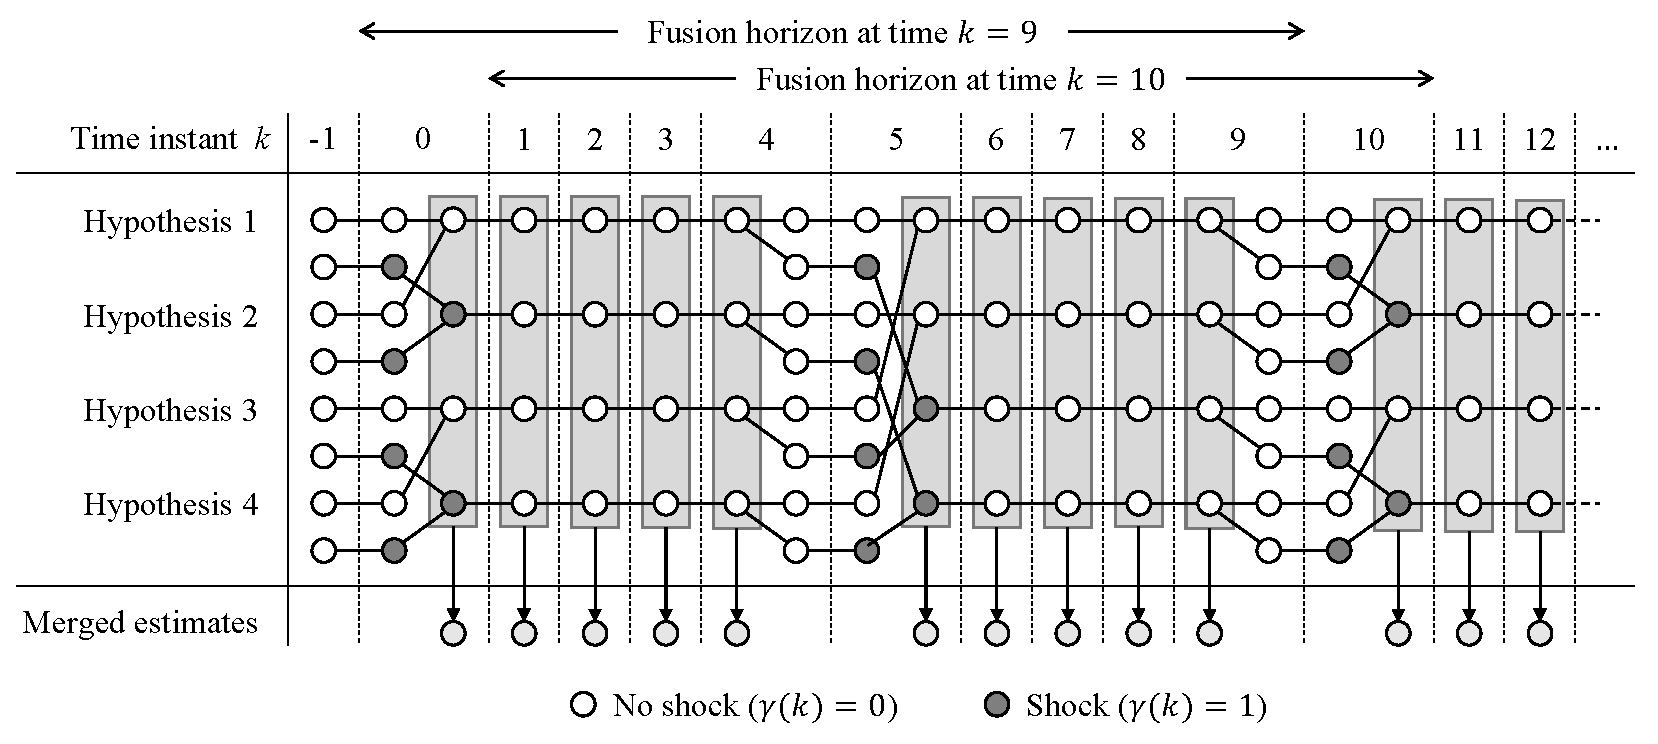
\includegraphics[width=15.5cm]{images/mm_obs_seq_sf95.pdf}
	\caption{Sequence branching and merging example ($N_f=10$, $n_\text{max}=2$, $d=5$)}
	\label{fig:mm-obs-seq-sf95}
\end{figure}

Rather than constant branching and merging indices, as in GPB2 (\ref{eq:Hbranch_GPB2}, \ref{eq:Hmerge_GPB2}), sequences of branching and merging indices are needed. In this example, they are
\begin{equation} \label{eq:Hbranch_SFex2}
	\mathcal{H}_{\text{branch}} = \begin{Bmatrix}
		\begin{bmatrix} 1 \\ 2 \\ 3 \\ 4 \end{bmatrix} &
		\begin{bmatrix} 1 \\ 2 \\ 3 \\ 4 \end{bmatrix} &
		\begin{bmatrix} 1 \\ 2 \\ 3 \\ 4 \end{bmatrix} &
		\begin{bmatrix} 1 \\ 2 \\ 3 \\ 4 \end{bmatrix} &
		\begin{bmatrix} 1 \\ 1 \\ 2 \\ 2 \\ 3 \\ 3 \\ 4 \\ 4 \end{bmatrix} &
		\begin{bmatrix} 1 \\ 2 \\ 3 \\ 4 \end{bmatrix} &
		\begin{bmatrix} 1 \\ 2 \\ 3 \\ 4 \end{bmatrix} &
		\begin{bmatrix} 1 \\ 2 \\ 3 \\ 4 \end{bmatrix} &
		\begin{bmatrix} 1 \\ 2 \\ 3 \\ 4 \end{bmatrix} &
		\begin{bmatrix} 1 \\ 1 \\ 2 \\ 2 \\ 3 \\ 3 \\ 4 \\ 4 \end{bmatrix}
	\end{Bmatrix},
\end{equation}
and
\begin{equation} \label{eq:Hmerge_SFex2}
	\mathcal{H}_{\text{merge}} = \begin{Bmatrix}
		\begin{bmatrix}	1 \\ 3 \end{bmatrix} & 1 & 1 & 1 & 1 & \begin{bmatrix}	1 \\ 5 \end{bmatrix} & 1 & 1 & 1 & 1 \\
		\begin{bmatrix}	2 \\ 4 \end{bmatrix} & 2 & 2 & 2 & 2 & \begin{bmatrix}	3 \\ 7 \end{bmatrix} & 2 & 2 & 2 & 2 \\
		\begin{bmatrix}	5 \\ 7 \end{bmatrix} & 3 & 3 & 3 & 3 & \begin{bmatrix}	2 \\ 6 \end{bmatrix} & 3 & 3 & 3 & 3 \\
		\begin{bmatrix}	6 \\ 8 \end{bmatrix} & 4 & 4 & 4 & 4 & \begin{bmatrix}	4 \\ 8 \end{bmatrix} & 4 & 4 & 4 & 4 \\
	\end{Bmatrix}.
\end{equation}

% Remove these: they don't add anything since these can be derived from the sequence
% and the branching/merging indices. Also, this convention for \Gamma_b and \Gamma_m
% was not defined. \Gamma_f was defined as single sequence and arguably would be
% better restricted to the merged sequences, than the branched ones.
%Likewise, the merged and branched shock (mode) indicator sequences are
%\begin{multline} \label{eq:Gamma_km09}
%	\glsadd{Gammafkmnk}\Gamma_m(0,9) = \left\{
%		\mathbf{\gamma}_m(0), \mathbf{\gamma}_m(1), \cdots, \mathbf{\gamma}_m(9)
%	\right\} = \\ 
%	\left\{
%		\begin{bmatrix} 0 \\ 1 \\ 0 \\ 1 \end{bmatrix},
%		\begin{bmatrix} 0 \\ 0 \\ 0 \\ 0 \end{bmatrix},
%		\begin{bmatrix} 0 \\ 0 \\ 0 \\ 0 \end{bmatrix},
%		\begin{bmatrix} 0 \\ 0 \\ 0 \\ 0 \end{bmatrix},
%		\begin{bmatrix} 0 \\ 0 \\ 0 \\ 0 \end{bmatrix},
%		\begin{bmatrix} 0 \\ 0 \\ 1 \\ 1 \end{bmatrix},
%		\begin{bmatrix} 0 \\ 0 \\ 0 \\ 0 \end{bmatrix},
%		\begin{bmatrix} 0 \\ 0 \\ 0 \\ 0 \end{bmatrix},
%		\begin{bmatrix} 0 \\ 0 \\ 0 \\ 0 \end{bmatrix},
%		\begin{bmatrix} 0 \\ 0 \\ 0 \\ 0 \end{bmatrix}
%	\right\}.
%\end{multline}
%\begin{multline} \label{eq:Gamma_kb09}
%		\Gamma_b(0,9 \mid 9) = \left\{\mathbf{\gamma}_b(0 \mid 0), \mathbf{\gamma}_b(1 \mid 1), \cdots, \mathbf{\gamma}_b(9 \mid 9) \right\} = \\
%		\left\{
%			\begin{bmatrix} 0 \\ 0 \\ 0 \\ 0 \end{bmatrix},
%			\begin{bmatrix} 0 \\ 0 \\ 0 \\ 0 \end{bmatrix},
%			\begin{bmatrix} 0 \\ 0 \\ 0 \\ 0 \end{bmatrix},
%			\begin{bmatrix} 0 \\ 0 \\ 0 \\ 0 \end{bmatrix},
%			\begin{bmatrix} 0 \\ 0 \\ 0 \\ 0 \\ 1 \\ 1 \\ 1 \\ 1 \end{bmatrix},
%			\begin{bmatrix} 0 \\ 0 \\ 0 \\ 0 \end{bmatrix},
%			\begin{bmatrix} 0 \\ 0 \\ 0 \\ 0 \end{bmatrix},
%			\begin{bmatrix} 0 \\ 0 \\ 0 \\ 0 \end{bmatrix},
%			\begin{bmatrix} 0 \\ 0 \\ 0 \\ 0 \end{bmatrix}
%			\begin{bmatrix} 0 \\ 0 \\ 1 \\ 1 \\ 0 \\ 0 \\ 1 \\ 1 \end{bmatrix},
%		\right\},
%\end{multline}
%\begin{multline} \label{eq:Gamma_kb110}
%		\Gamma_b(1,10 \mid 9) = \left\{ \mathbf{\gamma}_b(1 \mid 0), \mathbf{\gamma}_b(2 \mid 1), \cdots, \mathbf{\gamma}_b(10 \mid 9) \right\} = \\
%		\left\{
%			\begin{bmatrix} 0 \\ 1 \\ 0 \\ 1 \\ 0 \\ 1 \\ 0 \\ 1 \end{bmatrix},
%			\begin{bmatrix} 0 \\ 0 \\ 0 \\ 0 \end{bmatrix},
%			\begin{bmatrix} 0 \\ 0 \\ 0 \\ 0 \end{bmatrix},
%			\begin{bmatrix} 0 \\ 0 \\ 0 \\ 0 \end{bmatrix},
%			\begin{bmatrix} 0 \\ 0 \\ 0 \\ 0 \end{bmatrix},
%			\begin{bmatrix} 0 \\ 1 \\ 0 \\ 1 \\ 0 \\ 1 \\ 0 \\ 1 \end{bmatrix},
%			\begin{bmatrix} 0 \\ 0 \\ 0 \\ 0 \end{bmatrix},
%			\begin{bmatrix} 0 \\ 0 \\ 0 \\ 0 \end{bmatrix},
%			\begin{bmatrix} 0 \\ 0 \\ 0 \\ 0 \end{bmatrix},
%			\begin{bmatrix} 0 \\ 0 \\ 0 \\ 0 \end{bmatrix}
%		\right\}.
%\end{multline}
Although the number of branched hypotheses is time-varying, after $N_f$ time steps the sequences repeat such that
\nomenclature{$\mathbf{\gamma}_m(k)$}{vector of random shock indicators, $\gamma_f(k)$ for $f=1,2,...,m$, at time $k$}%
\begin{equation} \label{eq:rmkrmkmNf_SFex2}
	\mathbf{\gamma}_m(k) = \mathbf{\gamma}_m(k-N_f).
\end{equation}

As in the \gls{GPB2} algorithm, the overall estimates of the system states and outputs, $\hat{\mathbf{x}}(k \mid k)$ and $\hat{\mathbf{y}}(k \mid k)$, are calculated by merging the partially-merged estimates into one overall estimate. This is achieved by substituting $\mathbf{\hat{x}}_m(k \mid k)$ and $\mathbf{\hat{y}}_m(k \mid k)$ for $\mathbf{\hat{x}}_f(k \mid k)$ and $\mathbf{\hat{y}}_f(k \mid k)$ in \eqref{eq:xkyk_hat_MKF}.

\cite{robertson_detection_1995} described a systematic procedure to choose the parameters $N_f$, $n_\text{max}$, and $d$ and give the formula for the total probability of the modelled hypotheses as
\begin{equation} \label{eq:p_gamma}
	\beta=\operatorname{Pr}\left(\sum_{i=1}^{n} \gamma(i d) \leq n_\text{max} \right) = \sum_{j=0}^{n_\text{max}} \binom{n}{j} \varepsilon_d^{n-j}(1-\varepsilon_d)^{j},
\end{equation}
\nomenclature{$\beta$}{sequence fusion paramter: total probability of the modelled hypotheses, or in the case of the \acrshort{BRW}, a parameter of the additive bias function $a(\cdot)$}%
where $\binom{n}{j}$ represents the number of possible combinations of $j$ shocks in $n$ detection intervals. They recommended that the total probability should be at least 0.99 to ensure that only low-probability hypotheses are ignored.

In a later journal paper, \cite{robertson_method_1998} described a variation to the sequence fusion algorithm described above.  Rather than assuming that the shock occurs in the first sample period of each detection interval, as shown in Figures \ref{fig:mm-obs-seq-SFex1} and \ref{fig:mm-obs-seq-SFex2}, they proposed to represent the possibility of a shock as a sequence of $d$ smaller shocks such that the total variance over the detection interval is the same as that of one shock. They claimed this improved the performance of the algorithm in their simulations.

To implement this modification, define a new variable, $\delta(n)$, to represent whether or not at least one shock occurred during the $n$\textsuperscript{th} detection interval:
\nomenclature{$\delta(n)$}{sequence fusion variable: indicator of whether one or more shocks occurred in detection interval $n$}
\begin{equation} \label{eq:deltak}
	\delta(n) = \begin{cases*}
		0 & \text{if} $\sum_{k=(n-1) d}^{n d - 1}{\gamma(k)} = 0$, \\
		1 & \text{if} $\sum_{k=(n-1) d}^{n d - 1}{\gamma(k)} \ge 1$.
	\end{cases*}
\end{equation}

Then, replace the random shock variable used at each sample time, $w_p(k)$ \eqref{eq:wpk2}, with:
\begin{equation} \label{eq:wpdk}
	w_{p,d}(k) \sim 
	\begin{cases*}
		\mathcal{N}\left(0, \sigma_{w_p}^2\right) & \text{when} $\delta(n) = 0$, \\
		\mathcal{N}\left(0, \frac{b^2\sigma_{w_p}^2}{d}\right) & \text{when} $\delta(n) = 1$.
	\end{cases*}
\end{equation}

Note that the variance of a single shock, $b^2\sigma_{w_p}^2$, has ben divided by the detection interval length $d$. In this version of the algorithm, the branching and merging operations are only carried out at the end of each detection interval. In the steps within the detection interval, the Kalman filters are updated using the measurements, but no branching or merging occurs.

Figure \ref{fig:mm-obs-seq-sf98} shows the shock hypothesis sequences and the merging and branching steps of the 1998 version of the sequence fusion algorithm with the same parameters as in the previous example.
\begin{figure}[ht]
	\centering
	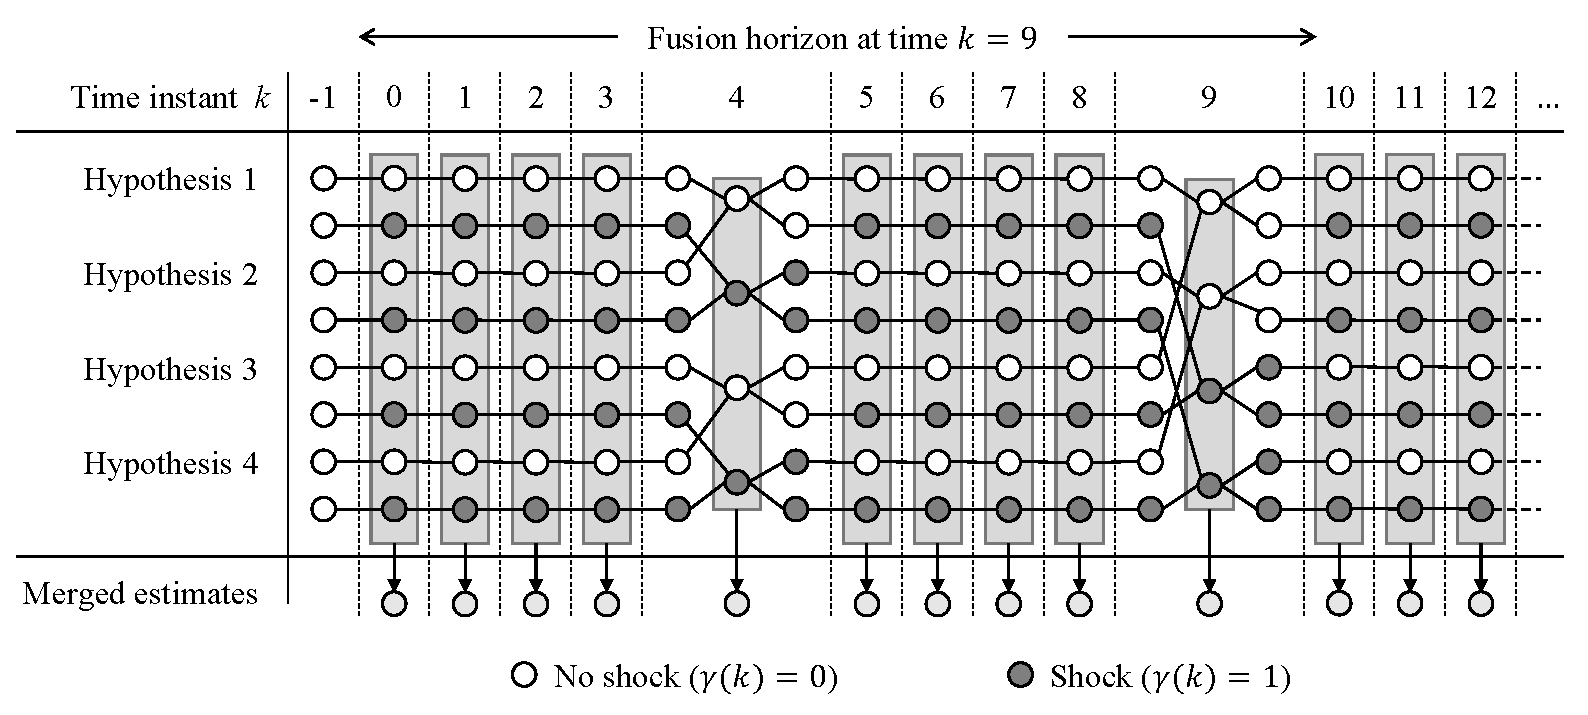
\includegraphics[width=15cm]{images/mm_obs_seq_sf98.pdf}
	\caption{Sequence branching and merging example – 1998 version ($N_d=5$, $n_\text{max}=2$, $N_f=10$)}
	\label{fig:mm-obs-seq-sf98}
\end{figure}
Note the two main differences when compared to Figure \ref{fig:mm-obs-seq-sf95}. Firstly, the system mode indicators are the same throughout the detection interval, whereas in the 1995 version the shocks were assumed to occur only at the first sample time of each detection interval. Secondly, after branching, the $n_h$ hypotheses are maintained for the duration of the detection interval before being merged and branched at the last sample time of the detection interval. The idea of these modifications is to allow $N_d$ Kalman filter updates to occur with the adjusted shock probability and variance (\ref{eq:p_gamma_d}, \ref{eq:wpdk}) before evaluating and merging the estimates. This was expected to produce better estimates of the hypothesis probabilities in situations where it takes more than one time step to detect changes in the system.

\subsubsection{Sequence pruning} \label{sec:pruning}

\textit{Sequence pruning} is the selective deletion of shock hypotheses that have a low likelihood given the current measurements. \cite{eriksson_classification_1996} used the \textit{adaptive forgetting through multiple models} (\acrshort{AFMM}) algorithm by \cite{andersson_adaptive_1985} for \gls{RODD} estimation. The \gls{AFMM} uses sequence pruning to limit the number of hypotheses and filters. The current hypotheses at each time instant are ranked according to their conditional probabilities \eqref{eq:Pr_Gammak_given_Yk}. The hypothesis with the lowest probability is then pruned with the caveat explained below. The most probable hypothesis is allowed to branch but all other hypotheses are advanced assuming no shock occurs in the next time period (i.e. all but one of their branches are pruned). This makes sense in the case of \gls{RODD} disturbances because the probability of a shock is low. Thus, the total number of hypotheses and filters is capped at a fixed number, $n_h$.

The caveat mentioned above, is that no hypothesis may be eliminated less than $N_\text{min}$ time steps after being created. This is to prevent good hypotheses from being eliminated before the conditional probabilities have been properly estimated, which can take more than one sample period. For this reason, $n_h$ must be at least sufficient to accommodate the \textit{minimum life}, $N_\text{min}$, of all new hypotheses. Note that in the case of systems with more than one \gls{RODD} disturbance, the number of branches of the most likely sequence is more than two, \hl{and the same number} of sequences will be pruned at each sample time.
\nomenclature{$N_\text{min}$}{sequence pruning parameter: minimum life of a branched hypothesis in number of sampling intervals}%

To illustrate the sequence pruning procedure, consider the diagram in Figure \ref{fig:mm-obs-seq-SP}. This shows one possible evolution of the hypothesis sequences in response to an actual shock sequence consisting of one shock at time $k=4$.  The most likely hypotheses at each time instant, identified by the circles with thicker outlines, branch into two at the next time instant. After the limit of five hypotheses is reached, one hypothesis is pruned at each sample time and replaced by a new branched hypothesis at the next. Note that at time $k=6$, hypothesis 2 becomes the most likely based on the available measurements at that time. Also note that no new branches are terminated in less than two sample times.
\begin{figure}[ht]
	\centering
	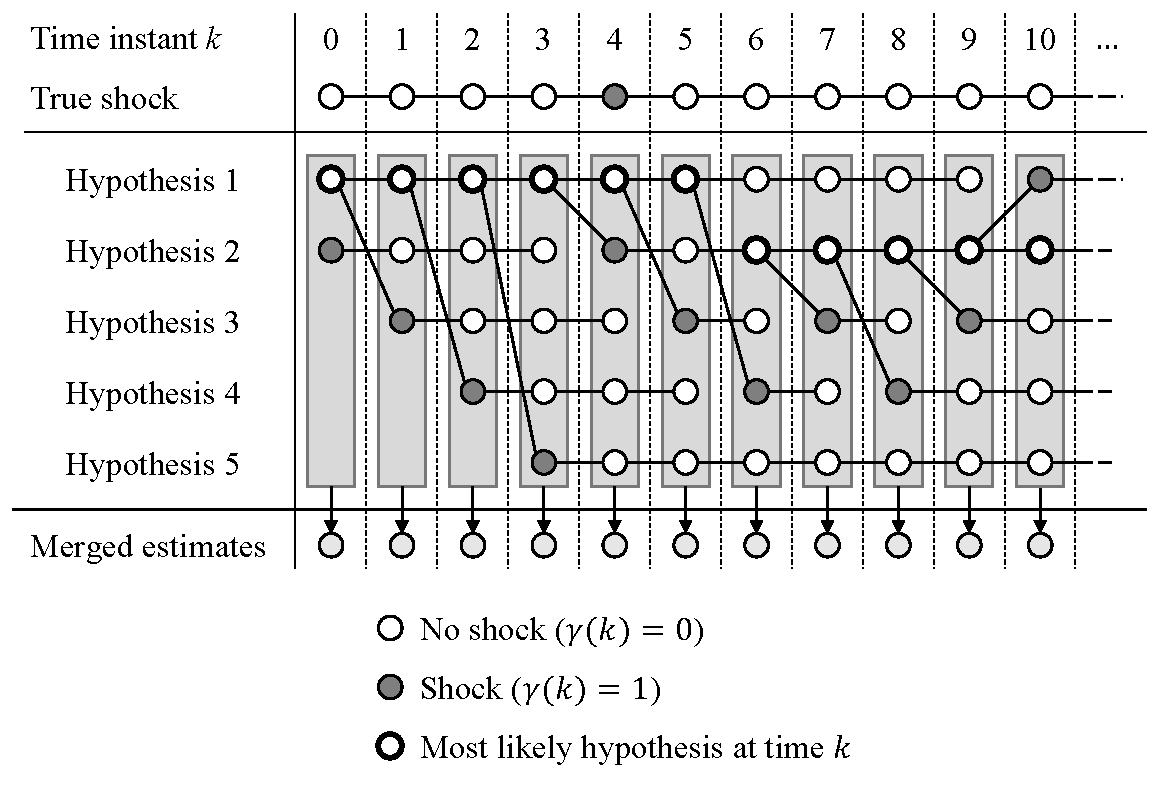
\includegraphics[width=10.7cm]{images/mm_obs_seq_SP.pdf}
	\caption{Sequence pruning example ($n_h=5$, $N_\text{min}=2$)}
	\label{fig:mm-obs-seq-SP}
\end{figure}

The \gls{AFMM} algorithm includes a complementary procedure for online estimation of the measurement noise covariance, $\mathrm{R}(k)$. This component was not implemented in this work since it is assumed that the variance of the measurement noise is time-invariant.

\subsubsection{Implementation details} \label{sec:implementation}

The diagram in Figure \ref{fig:mkf-infoflow} depicts the general computation steps and information flows of the sub-optimal multiple-model observers, as implemented in this work. The solid black rectangles represent computation steps and the \hl{coloured lines} represent the main variables. Steps 1 and 2 are the prediction steps of the Kalman filters (\ref{eq:xfkp1_hat}, \ref{eq:yfk_pred}), step 3 is the calculation of the prior probabilities of the hypotheses \eqref{eq:Pr_Gammak_given_Ykm1}, step 4 is the hypotheses evaluation step (\ref{eq:Pr_Gammak_given_Yk}, \ref{eq:qfk}), and step 5 is the Kalman filter update step (\ref{eq:xfkyfk_hat}, \ref{eq:Pkf-stab}). Step 6 is a place-holder for the sub-optimal procedures which depend on the specific algorithm but in this work include some combination of sequence branching, pruning, and merging. During this step, the final estimates of the states and outputs are also calculated.

\begin{figure}[ht]
	\centering
	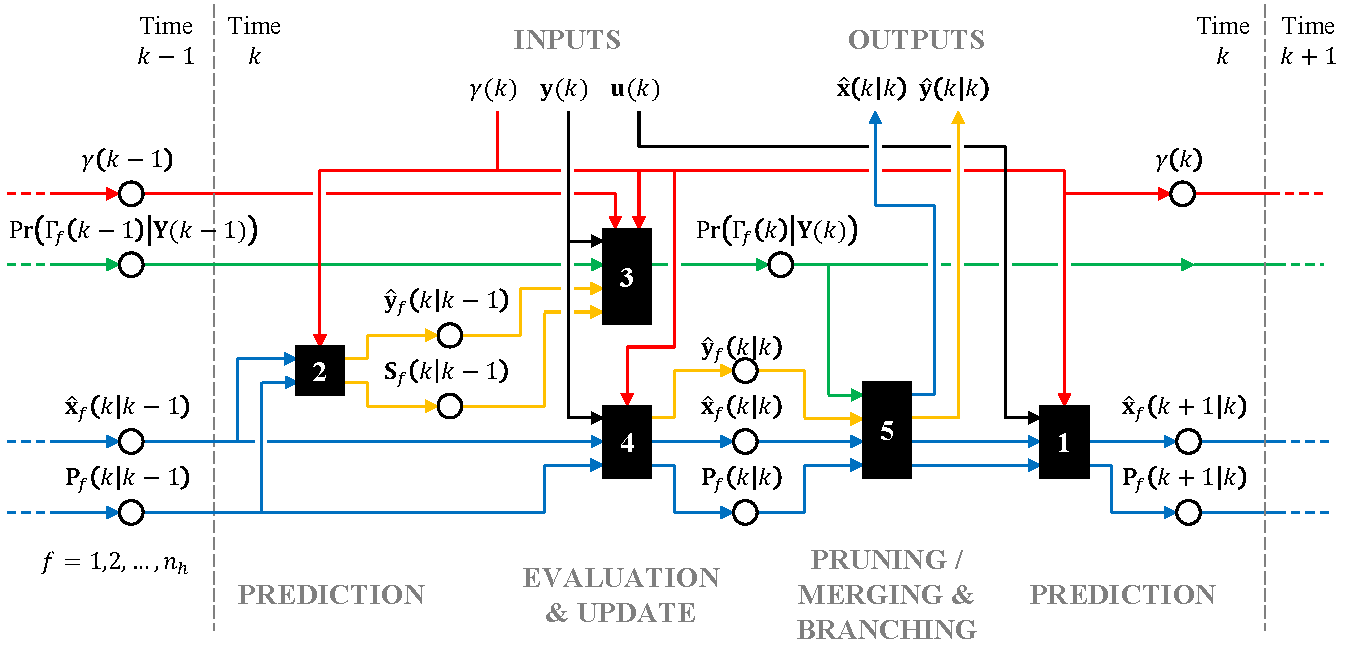
\includegraphics[width=15.5cm]{images/mkf_infoflow.pdf}
	\caption{General information flow diagram of a multiple-model observer}
	\label{fig:mkf-infoflow}
\end{figure}

At time $k$, the algorithm requires a mode indicator vector, $\gamma(k)=\begin{bsmallmatrix} \gamma_1(k) & \cdots & \gamma_{n_h}(k) \end{bsmallmatrix}^\intercal$, the system output measurement, $\mathbf{y}_M(k)$, and input, $\mathbf{u}(k)$, and produces estimates of the states, $\hat{\mathbf{x}}(k \mid k)$, and outputs, $\hat{\mathbf{y}}(k \mid k)$. The mode indicator vector is either constant, as in the case of the \gls{GPB1} and \gls{GPB2} algorithms or is specified by the sub-optimal procedure at each time step. At the end of each time step, the mode indicator vector, conditional hypothesis probabilities, one-step-ahead state predictions, and the prediction error covariances for each hypothesis are stored for use in the next time step. The sub-optimal algorithm, which determines $\gamma(k)$ as well as the merging, pruning, and branching procedures in step 6, may have other variables that need to be stored. These are not shown on the diagram. The total number of hypotheses modelled, $n_h$, also depends on the algorithm, and may be time-varying.

\section{System identification} \label{sec:sys-id}

% Some text not used in IFAC report
Model-based observers such as the Kalman filter require a dynamic model of the process. In practice, models of the process dynamics are not available but they can be identified when input-output data sampled from the process is available. In this case, system identification methods are common practice, as described by \cite{ljung_system_1999} among others.

To construct a multiple-model observer for systems with \gls{RODD}s, the structure and parameters of the disturbance model as well as the process model are needed. \gls{RODD}s are discrete-time \acrlong{MJLS} (\acrshort{MJLS}) \citep{costa_discrete-time_2005}. Standard approaches to system identification such as least-squares regression are not applicable to hybrid dynamical systems with both discrete and continuous states. Identification of these types of systems is challenging and the subject of ongoing research. See for example, \cite{piga_estimation_2020}.

%Outline notes:
%\begin{itemize}
%	\item Explain Isaksson and Eriksson's perspective on standard system identification approach.
%	\item Explain distinction between system detection or `discrimination' and system identification, reference Isaksson and Eriksson's paper on disturbance classification (whether disturbance at input or output of process).
%	\item Introduce other approaches—MLE, EM algorithm (Dempster et al., Wong \& Lee)
%	\item Methods proposed by Bemporad (Fitting jump models, 2018 and Jump Box-Jenkins, 2020).
%	\item Theory and challenges Costa book. Others?
%	\item In recent years, numerical methods to overcome the intractability of the probabilistic integral have received a lot of attention.
%	\item Sequential Monte-Carlo methods, (incl. particle filtering), Stochastic Variational Inference, ... (read Special issue in IEEE control magazine for an overview of these methods)
%\end{itemize}

% More text from IAFAC paper:
%are assumed to be known and were set to match the characteristics of the simulated disturbance. In practice, they would have to be estimated, either using prior knowledge of the disturbance source, or possibly from system output measurements using an appropriate system identification method---see \cite{schon_sequential_2015} for one possible approach---provided a sufficiently long sequence of data is available.

% Note: may remove this if we aren’t using any formal methods.

%\section{Control strategies}
%
%In this work, the goal is to test the performance of different observers in a closed-loop feedback control application (not to evaluate different control strategies). Therefore, only one control strategy is considered. According to the \textit{separation principle} of estimation and control, the control strategy may be designed independently of the observer. The controller is designed using the same augmented system model, including the plant model and disturbance models, that is used in the observer design. However, the switching behaviour of the random shock variable used in the \gls{RODD} is not explicitly considered in the control design. The estimates of the model states produced by the observer are assumed to be optimal, i.e. the expected values, and their uncertainty is not taken into account by the control algorithm or in its design.
%
%
%\subsection{Model predictive control}
%
%\textit{\acrlong{MPC}} (\acrshort{MPC}) is a well known and widely used multi-variable control algorithm used in industrial applications. This is largely due to the fact that constraints can be imposed on the manipulated variables and control variables, as well as its intuitive design and the ease with which it can be tuned to achieve control objectives \citep{maciejowski_predictive_2002}. Although it is a computationally complex algorithm, numerous proven commercial products exist to enable its implementation.
%
%\gls{MPC} utilizes a prediction equation based on the dynamic model of the system to find feasible future trajectories of the system outputs as a function of the manipulated variables and the states of the model at the current time. The length of the prediction horizon, \gls{Hp}, is defined in terms of the number sample times starting at the next time instant, $k+1$. The predicted outputs over the prediction horizon, calculated at the current time $k$, are denoted $\hat{\textbf{y}}(k+i | k)$ for $i=1,2,...,H_p$. The length of the control horizon, \gls{Hc}, is defined starting at the current time, $k$, and the manipulated inputs are denoted $\mathbf{u}(k+i-1)$ for $i=1,2,...,H_c$. The control horizon is usually shorter than the prediction horizon, in which case, $\mathbf{u}(k+j)=\mathbf{u}(k+H_c-1)$ for $j=H_c,H_c+1,...,H_p$.
%
%The constrained optimization problem, which is solved at each time step, is
%\begin{align} \label{eq:mpc-opt}
%	\begin{split}
%		\min _{\mathbf{u}(k), \mathbf{u}(k+1), \ldots, \mathbf{u} (k+H_c-1)}
%		& \quad \sum_{i=1}^{H_{p}}[\mathbf{\hat{y}}(k+i / k) - \mathbf{r}(k+i)]^\intercal \mathbf{\Phi} [\mathbf{\hat{y}}(k+i / k) - \mathbf{r}(k+i)] \\
%		& \qquad + \sum_{i=1}^{H_{c}}[\Delta \mathbf{u}(k+i-1)]^\intercal \mathbf{\Lambda} [\Delta \mathbf{u}(k+i-1)] \\
%			\end{split} \\
%		\text { subject to: }
%		&\ \mathbf{u}_{min} \leq \mathbf{u}(k+j-1) \leq \mathbf{u}_{max} \quad  j=1,2, \dots, H_{c} \label{eq:mpc-cons-1}, \\
%		& \Delta \mathbf{u}_{min} \leq \Delta \mathbf{u}(k+j-1) \leq \Delta \mathbf{u}_{max} \quad j=1,2, \dots, H_{c}, \label{eq:mpc-cons-2} \\
%		& \mathbf{y}_{min} \leq \mathbf{\hat{y}}(k+j / k) \leq \mathbf{y}_{max} \quad  j=1,2, \dots, H_{p}, \label{eq:mpc-cons-3}
%\end{align}\textbf{[TODO: Consider including slack variables to ensure feasibility]}
%where $\mathbf{r}(k+i)$ for $i=1,2,...,H_p$ is the reference output trajectory, and $\Delta \mathbf{u}(k)$ is the change in the manipulated variable at time $k$, defined as $\Delta \mathbf{u}(k) = \mathbf{u}(k) - \mathbf{u}(k-1)$. The tunable parameters are $H_p$, $H_c$, $\mathbf{\Phi}$, and $\mathbf{\Lambda}$, and the constraints are $\mathbf{u}_{min}$, $\mathbf{u}_{max}$, $\Delta \mathbf{u}_{min}$, $\Delta \mathbf{u}_{max}$, $\mathbf{y}_{min}$, and $\mathbf{y}_{max}$. Note that the last constraint \eqref{eq:mpc-cons-3} only guarantees that the estimate of the system output will not violate the constraints. This does not imply that the true system output will respect them at all times.
%
%Once a solution to the optimization problem is found, only the control actions at the current time, $\mathbf{u}(k)$, are transmitted to the plant. The procedure is then repeated every future time instant to compute the subsequent control actions. This is referred to as \textit{receding horizon control}.


\section{Grinding simulation model} \label{sec:grinding-simulator}

%Outline notes:
%\begin{outline}
%    \1 Assumptions and limitations: constant breakage rate model, relationships between speed, media, trajectories, filling level and breakage not captured.
%	\1 Describe grate, transport delays and cyclone model.
%	\1 Outline any significant changes made from Edgar's model
%	\1 Figure: simulation results showing steady-state characteristics - e.g. power, grind, and throughput vs. fill level and speed.
%	\1 Figure \ref{fig:coarse_fine_psd_plot}: Particle size distributions of feed, recirculating load and product - this should help explain steady-state characteristics.
%	\1 Figure - Step responses of main process variables to changes in ore properties.
%	\1 Selection of particle size distribution as the disturbance variable for this work.
%	\1 Steady-state characteristics with operating points (grind curves)\\
%\end{outline}

A dynamic simulation model of the primary grinding circuit of a gold mine in Quebec is used to simulate the effects of changes in ore feed properties on the grinding circuit over time. The model was developed by \cite{perez_garcia_dynamic_2020} following the methodology described by \cite{grimble_dynamic_2010} and was calibrated to match operating data collected from the plant \citep{perez-garcia_systematic_2020}. Grinding in the \acrshort{SAG} mill is simulated by a \textit{population balance model} with 24 discrete ore particle size intervals and constant specific-energy selection rates (i.e. breakage rates are proportional to total energy consumption) and a constant breakage matrix.

Figure \ref{fig:sag-diag} is a simplified diagram of the simulated \acrshort{SAG} mill, which is in a closed circuit consisting of a feed conveyor, pump box, pump, and a bank of hydro-cyclones.
\begin{figure}[ht]
	\centering
	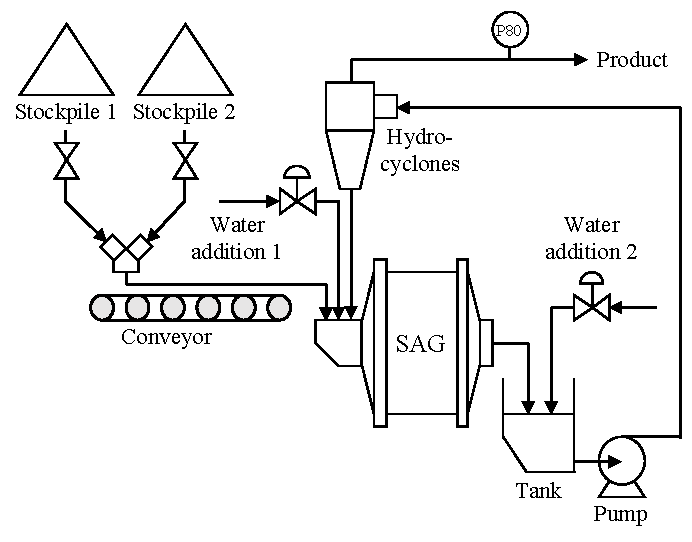
\includegraphics[width=12.5cm]{images/sag-circuit-diag.pdf}
	\caption{Simplified process flow diagram}
	\label{fig:sag-diag}
\end{figure}
For the purposes of this work, two ore feed streams with different \gls{PSD}s were simulated. Each stream is a different mix of two different ores. One ore has a fine \gls{PSD} and the other is coarse. The mix for stream \#1 (`mix 1') consists of 22.83\% coarse ore (\textit{mix factor} of 0.2283) and mix \#2 is an even mix of both ores (mix factor of 0.5). The two streams are mixed before discharging onto the conveyor. Figure \ref{fig:coarse_fine_psd_plot} shows the \gls{PSD}s of the two mixtures.
\begin{figure}[ht]
	\centering
	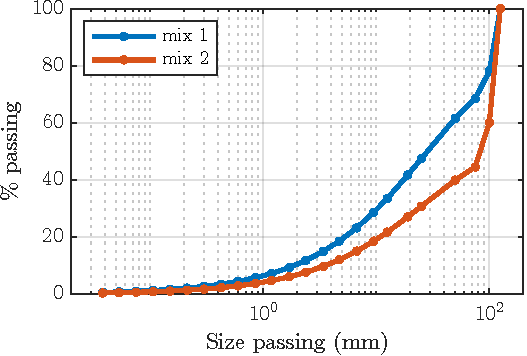
\includegraphics[width=9cm]{images/coarse_fine_cumpsd_plot.pdf}
	\caption{Ore particle size distributions}
	\label{fig:coarse_fine_psd_plot}
\end{figure}

The simulated instrumentation is also illustrated in Figure \ref{fig:sag-diag}. \hl{The setpoint of the water addition flowrate to the mill inlet (`water addition 1') is set to a fixed ratio of the ore feed rate.} The pump-box \hl{(`tank')} has a \gls{PI} controller to control the level to a fixed set-point by manipulating the water addition flow rate set-point (`water addition 2'). The main process variable used in this work is the product P80 measurement, which is a simulated online analyser that estimates the 80\% passing size of the material \hl{in the slurry} leaving the circuit. In this work, the inlet water addition ratio, the conveyor speed, the discharge pump speed, and the mill rotational speed are all fixed.

%The simulated instrumentation is also illustrated in Figure \ref{fig:sag-diag}. The \acrshort{SAG} mill water addition set-point is set by ratio control to a fraction of the fresh ore feed rate, which is measured on the conveyor. This water addition ratio is also manipulated. The pump-box level has a PI (proportional-integral) controller to control the level to a fixed set-point by manipulating the water addition flow rate set-point. The discharge pump speed is fixed. Conveyor speed is adjusted automatically in response to the fresh ore feed rate set-point. The \acrshort{SAG} rotational speed set-point may also be manipulated.
%
%The measurable process variables used in this work are the mill weight, which includes the weight of the shell and liners as well as the mill contents, mill power consumption, the solids-content of the cyclone feed stream, and the particle size (P80) of the ground product in the cyclone overflow. Mill filling level and other simulation variables are available for analysis but are assumed to be unmeasured in the real operation and therefore not available for process control.  Figure \ref{fig:grind_sim_io_diag} summarizes the inputs and outputs of the simulation model. Table \ref{tb:grind-vars} lists the normal operating points, units, and minimum and maximum operating limits of each variable.
%
%%TODO: Table of process variables and normal operating points, limits etc.
%\begin{table}[ht]
%	\centering
%	\caption{Grinding simulation model inputs and outputs} \label{tb:grind-vars}
%	% See: https://texblog.org/2019/06/03/control-the-width-of-table-columns-tabular-in-latex/
%	% Also: https://www.overleaf.com/learn/latex/Tables
%	\begin{tabular}{c c >{\raggedright}p{5.5cm} c c c c}
%		%\toprule
%		& Label & Description & Op. pt. & Units & Min. & Max \\
%		\midrule
%		\multicolumn{7}{l}{\textit{manipulated variables}} \\
%		%\midrule
%		  & MV1       & Ore feed rate & 122.7 & tons/h & 0 & 200 \\   
%		  & MV2       & Mill speed (fraction of critical speed) & 0.77 & - & 0 & 0.85 \\ 
%		  & MV3       & Water addition ratio (fraction of ore feed rate) & 0.341 & - & 0 & 1 \\ 
%		%\midrule
%		\multicolumn{7}{l}{\textit{Unmeasured disturbance input}} \\
%		%\midrule
%		  & UD1        & Ore mix factor & 0.2283 & - & 0 & 1  \\ 
%		%\midrule
%		\multicolumn{7}{l}{\textit{Output variables}} \\
%		%\midrule
%		  & OV1        & Mill weight & 279.4 & tons & 100 & 320  \\ 
%		  & OV2       & Mill power consumption & 2391 & kW & 0 & 2400  \\ 
%		  & OV3       & Cyclone feed solids fraction & 61.4 & \% & 50 & 70  \\ 
%		  & OV4       & Cyclone overflow P80 & 105.4 & \% & 0 & 200  \\ 
%		\bottomrule
%	\end{tabular}
%\end{table}

%To better understand the relationships between the input and output variables, a set of simulations were carried out to determine steady-state operating conditions in the vicinity of the normal operating point. Figure \ref{fig:grind_sim_ss_plot1} shows how the steady-state values of the four output variables are affected by changes in the mill fill level (fraction of internal volume occupied by the charge) and rotation speed. The normal operating points are also shown, represented by solid markers. For these simulations, a simple PI controller was used to control the mill filling level by manipulating the ore feed rate and each simulation was run until all variables converged to steady-state values. However, no constraints were imposed during these simulations, therefore power consumption exceeds the maximum possible in some cases.
%
%These results are equivalent to the grind curves proposed by \cite{powell_applying_2009} for evaluating steady-state characteristics and optimal operating points for \acrshort{SAG} mills. However, compared to the curves presented by \cite{powell_applying_2009}, which were based on measurements from real operations, these are noticeably much closer to straight lines (i.e. linear relationships).
%
%A similar set of simulations were carried out to understand the effect of changing the ore mix factor on the steady-state values of the output variables. The results are shown in Figure \ref{fig:grind_sim_ss_plot2}. From these it can be seen that the change in ore mix has no effect on the steady-state power consumption of the mill. However, there are changes in the steady-state throughput (ore feed rate), cyclone feed solids fraction, and product particle size. The throughput is approximately 4 tons-per-hour higher and the product particle size is 1.5 microns smaller when the ore mix contains the higher fraction (0.5) of coarse ore.
%
%\begin{figure}[ht]
%	\centering
%	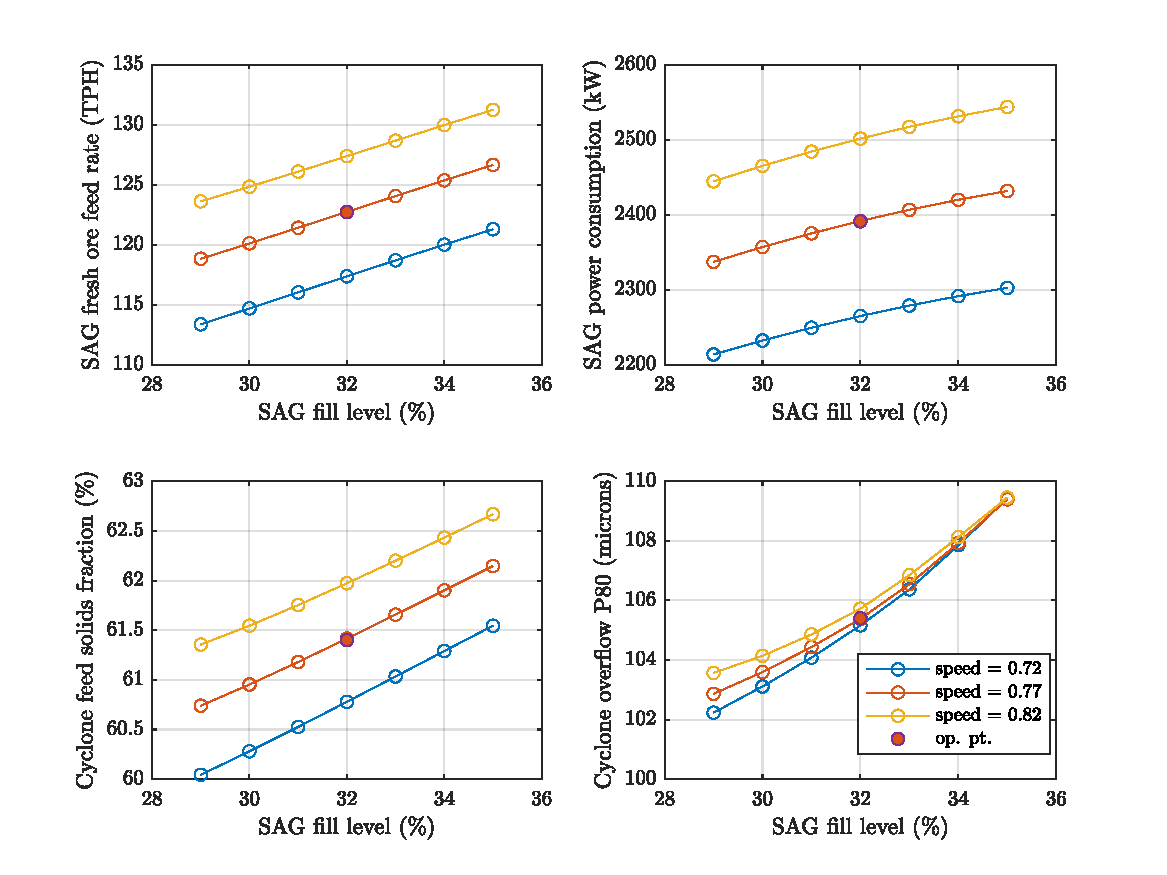
\includegraphics[width=15cm]{images/grind_sim_ss_plot1.pdf}
%	\caption{Steady-state operating points}
%	\label{fig:grind_sim_ss_plot1}
%\end{figure}
%
%\begin{figure}[ht]
%	\centering
%	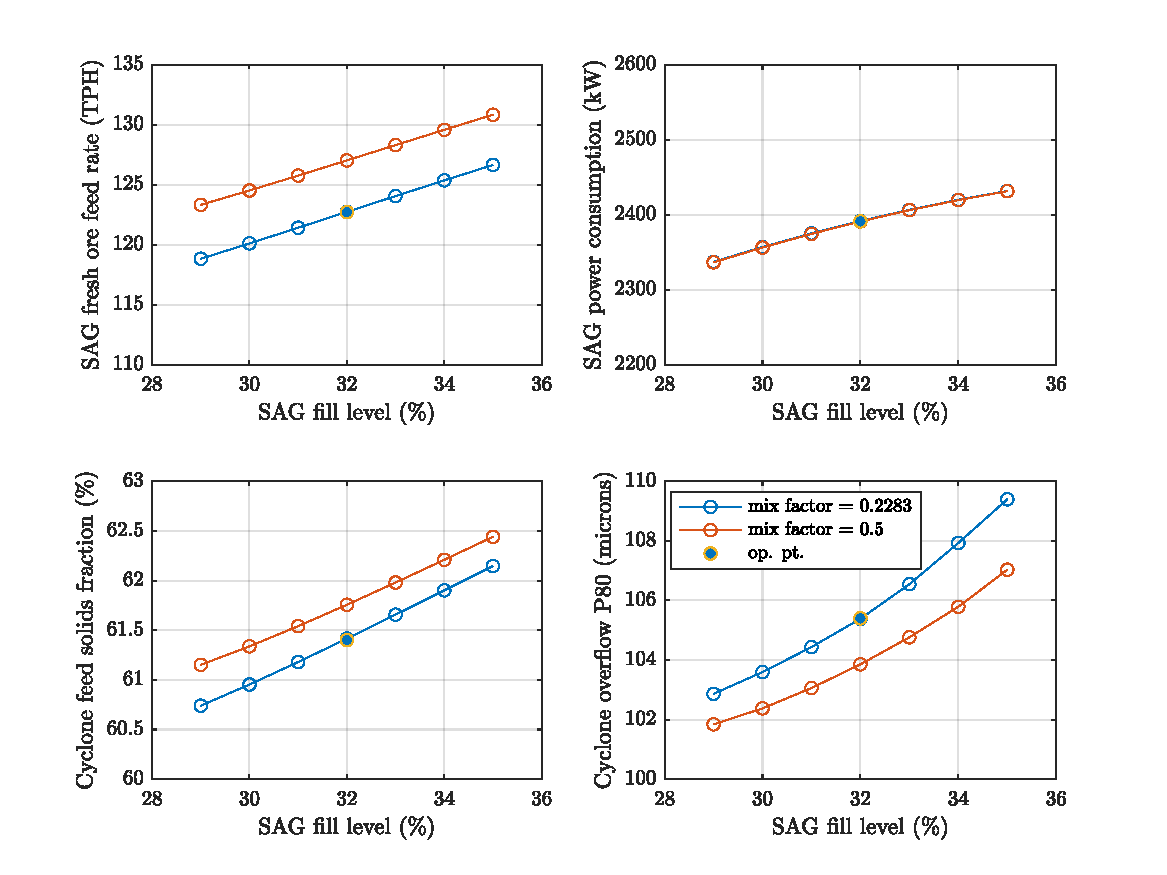
\includegraphics[width=15cm]{images/grind_sim_ss_plot2.pdf}
%	\caption{Effect of ore mix factor on steady-state operating points}
%	\label{fig:grind_sim_ss_plot2}
%\end{figure}

%Zero-mean Gaussian measurement noises are added to the outputs of the simulation model to simulate measurement errors. The standard deviations of these noises are shown in Table \ref{tb:meas-noise}. Except for the measurement noises and the input disturbance described above, the model itself is deterministic.

% Scaling factors
% 2
%& 0.0085
%& 0.01
%& 0.01
%& 2.2
%& 24
%& 0.2
%& 2
%
%\begin{table}[h!]
%	\centering
%	\caption{Simulated output measurements} \label{tb:meas-noise}
%	\begin{tabular}{c >{\raggedright}p{5.5cm} c c}
%		Label & Description & Sampling period (hours) & Noise std. dev. \\
%		\midrule
%		CV1        & Mill weight & 0.05 & XX \\ 
%		CV2       & Mill power consumption & 0.05 & XX \\ 
%		CV3       & Cyclone feed solids fraction & 0.05 & XX \\ 
%		CV4       & Cyclone overflow P80 & 0.05 & XX \\ 
%		\bottomrule
%	\end{tabular}
%\end{table}
%
%
%Although some of these process variables would likely be sampled at higher rates in practice, it is assumed, for simplicity, that they are all sampled at the same rate of 1 sample every 3 minutes (i.e. a sampling period of 0.05 hours). This was deemed to be a typical sampling rate of a standard online particle size analyser that might be used for the P80 measurement.


\section{Performance evaluation} \label{sec:evaluation}

Various metrics are used in this work to evaluate the performance of the observers. Since a simulation model of the plant is used and the input disturbances are also simulated, the true values of the system inputs and outputs (i.e. without measurement errors) are available.

The first metric is the \textit{\acrlong{RMSE}} (\acrshort{RMSE}) of the system output estimates, which is an indication of the magnitude of the differences between the estimates of an output signal, $\hat{Y}_i(N)=\left\{\hat{y}_i(1),\hat{y}_i(2), ..., \hat{y}_i(N)\right\}$, and its true values, $Y_i(N)=\left\{y_i(1),y_i(2), ..., y_i(N)\right\}$, (i.e. the output estimation errors),
\nomenclature{$\hat{Y}_i(k)$}{estimates of system output $i$ from time 0 to time $k$}%
\nomenclature{$\hat{\mathbf{Y}}(k)$}{system output estimates from time 0 to time $k$}%
\nomenclature{$Y_{i}(k)$}{system output $i$ from time 0 to time $k$}%
\nomenclature{$Y_{M,i}(k)$}{measurements of system output $i$ from time 0 to time $k$}%
\nomenclature{$\mathrm{RMSE}(\hat{Y},Y)$}{\acrlong{RMSE} of the output estimates, $\hat{Y}(N)$, from a simulation, compared to the true system outputs, $Y(N)$}%
\nomenclature{$\mathrm{RMSE}(\hat{Y},Y_M)$}{\acrlong{RMSE} of the output estimates, $\hat{Y}(N)$, from a simulation, compared to the system output meaurements, $Y_M(N)$}%
\begin{equation} \label{eq:rmse-calc-yest}
	\newcommand{\RMSE}{\textrm{RMSE}}
	\RMSE(\hat{Y}_i(N),Y_i(N)) = \sqrt{\frac{1}{N}\sum_{k=1}^{N}{(\hat{y}_i(k)-y_i(k))^2}}.
\end{equation}

Similarly, the \gls{RMSE} of the estimates of an unmeasured input disturbance signal, $\hat{p}_i(k)$, is
\begin{equation} \label{eq:rmse-calc-pest}
	\newcommand{\RMSE}{\textrm{RMSE}}
	\RMSE(\hat{P}_i(N),P_i(N)) = \sqrt{\frac{1}{N}\sum_{k=1}^{N}{(\hat{p}_i(k)-p_i(k))^2}}.
\end{equation}
 
As well as the overall \gls{RMSE}, two additional metrics are used to evaluate observer performance on systems with \gls{RODD}s. The \gls{RMSE} \textit{in transition}, which is the \gls{RMSE} during a period after a random shock, is used to evaluate the response of an observer to infrequent, abrupt disturbances. The transition period is defined as the samples occurring within $t_{\pm5\%}$ hours of the disturbance arriving at the input to the process, where $t_{\pm5\%}$ is the \textit{settling time} \hl{of the process}, defined as the time taken for the outputs to converge to within $\pm5\%$ of the final steady-state values. The \gls{RMSE} \textit{in steady-state} is defined as the samples occurring more than $t_{\pm5\%}$ hours after a disturbance and before the next one occurs.
\nomenclature{$t_{\pm5\%}$}{settling time of the process to within $\pm5$ percent of steady-state}%

The fourth metric is the \textit{\acrlong{RMSD}} (\acrshort{RMSD}) in the estimates,
\nomenclature{$\mathrm{RMSD}(\hat{Y})$}{\acrlong{RMSD} of the output estimates, $\hat{Y}(N)$, from a simulation}%
\begin{equation} \label{eq:rmsd-calc-yest}
	\newcommand{\RMSD}{\textrm{RMSD}}
	\RMSD(\hat{Y}_i(N)) = \sqrt{\frac{1}{N}\sum_{k=1}^{N}{(\hat{y}_i(k)-\hat{y}_i(k-1))^2}}.
\end{equation}
\nomenclature{$\mathrm{Var}(\hat{Y})$}{Variance of the output estimates, $\hat{Y}(N)$, from a simulation}%

This is a measure of the magnitude of high frequency changes in the estimates, which is an indication of the sensitivity of an observer to measurement noise.

\hl{A fifth metric is used in the case of the grinding simulator experiments, the variance of the estimates during steady-state periods. This is similar to the {\gls{RMSE}} in that it gives an indication of the sensitivity of the estimates to measurement noise.}
% Variance calc - only used in grinding model simulations
\begin{equation} \label{eq:var-calc}
	\begin{aligned}
		\newcommand{\Var}{\textrm{Var}} 
		\Var(\hat{y}(k)) = \frac{1}{N}\sum_{k=1}^{N}{(\hat{y}(k)-\mu_y)^2} \\
		\mu_y = \frac{1}{N}\sum_{k=1}^{N}{\hat{y}(k)}
	\end{aligned}
\end{equation}

To simplify notation, the argument $N$, indicating the length of the time series, is not always shown. Thus, $\textrm{RMSE}(\hat{Y}_i(N),Y_i(N))$ may be denoted $\textrm{RMSE}(\hat{Y}_i,Y_i)$. The capitalization of $Y$ indicates that it is a time series. Also, for \gls{SISO} systems, the subscript $i$ is redundant and dropped. Thus, $\textrm{RMSE}(\hat{Y},Y)$ is the \gls{RMSE} of the output of a system with only one output variable. However, $\textrm{RMSE}(\hat{\mathbf{Y}},\mathbf{Y})$ is used for a system with more than one output. The assumption is that this is the \gls{RMSE} averaged over all output signals, $Y_i(N)$ for $i=1, ..., n_y$.
% Removed since not doing control simulations.
%To evaluate the potential benefits of the observers in process control applications, simulations were carried out with an observer, a simulated controller, and the simulated process in closed-loop. In these cases, the \gls{RMSE}s of the control variables, $y_i(k)$, compared to a set of reference values, $R_i(N)$, is calculated to evaluate the performance of the control system,
%\begin{equation} \label{eq:rmse-calc-y}
%	\newcommand{\RMSE}{\textrm{RMSE}}
%	\RMSE(Y_i(N),R_i(N)) = \sqrt{\frac{1}{N}\sum_{k=1}^{N}{(y_i(k)-r_i(k))^2}}.
%\end{equation}
%
%In addition, the RMSD of the control actions, $u_i(k)$, is calculated to provide an indication of the sensitivity of the control system to measurement noise,
%\begin{equation} \label{eq:rmsd-calc-u}
%	\newcommand{\RMSD}{\textrm{RMSD}}
%	\RMSD(U_i(N)) = \sqrt{\frac{1}{N}\sum_{k=1}^{N}{(u_i(k)-u_i(k-1))^2}}.
%\end{equation}

Because the processes simulated in this work are stochastic, it is important to evaluate state estimators over sufficiently long simulation time periods to ensure that the results are close to the true average performance and are independent of the specific pseudo-random inputs generated for each simulation. This is particularly important when evaluating systems with \gls{RODD}s because the shocks occur infrequently. As an added precaution, identical random inputs are used when comparing the performance of two or more observers on the same system.

\hljb{In this chapter, the main methods and notation used in this work were introduced. The main disturbance model considered is the {\gls{RODD}} model ({\ref{eq:RODD}}), however, two additional disturbance models were presented, a more general switching model based on the HMM ({\ref{eq:MJLS}}) and the {\gls{BRW}} ({\ref{eq:brw}}). The standard Kalman filter (filtering form) was introduced, along with the multiple-model Kalman filter for estimation of switching systems. The two main sub-optimal algorithms used for {\gls{RODD}} estimation are a sequence fusion algorithm} {\citep{robertson_detection_1995, robertson_method_1998}} \hljb{(two versions of it), and a sequence pruning algorithm} {\citep{eriksson_classification_1996}}, \hljb{with implementation details. The grinding simulation model used to simulate a realistic grinding circuit was also introduced. Finally, the metrics used to evaluate the performance of observers were defined. The next chapter describes a series of simulations carried out to evaluate these observers.}% !TEX encoding = UTF-8 Unicode
\chapter{Methods}
\label{chap-methods}

\section{Disturbance models}

\subsection{Randomly-occurring deterministic disturbances} \label{sec:RODD}

\Acrlong{RODD}s (\acrshort{RODD}s) \citep{macgregor_duality_1984} are a family of stochastic process models suitable for simulating various types of infrequently-occurring disturbances in discrete-time.  The structure of the \gls{RODD} model is
\begin{equation} \label{eq:RODD}
	p(k) = \frac{B(q^{-1})}{A(q^{-1})} w_p(k),
\end{equation}
where $p(k)$ is the generated disturbance signal, $A(q^{-1})$ and $B(q^{-1})$ are polynomial functions of the backward shift operator, $q^{-1}$, and $w_p(k)$ is a random variable generated by a switching system.
\nomenclature{$p(k)$}{disturbance signal at time $k$}%
\nomenclature{$q^{-1}$}{backward shift operator}%
\nomenclature{$A(q^{-1})$}{\acrshort{RODD} model parameter: polynomial function of the backward shift operator}%
\nomenclature{$B(q^{-1})$}{\acrshort{RODD} model parameter: polynomial function of the backward shift operator}%
\nomenclature{$w_p(k)$}{random shock signal at time $k$}%
% One way to make links: \hyperlink{sym.pk}{$p(k)$}.

To generate randomly-occurring disturbances, the switching system,
\begin{equation} \label{eq:wpk1} 
	w_p(k) \sim 
	\begin{cases*}
		0 & with probability $1-\varepsilon$, \\
		\mathcal{N}\left( 0, \sigma_{w_p}^2 \right) & with probability $\varepsilon$,
	\end{cases*}
\end{equation}
\nomenclature{$\varepsilon$}{\acrshort{RODD} model parameter: probability of a random shock}%
may be used, where $w_p(k)$ is either 0 or is sampled from the normal distribution, $\mathcal{N}(0,\sigma_{w_p}^2)$, with mean zero and variance $\sigma_{w_p}^2$.  When the probability $\varepsilon$ is low ($\varepsilon<<1$), this system produces infrequent shocks.
\nomenclature{$\mathcal{N}(\mu,\sigma^2)$}{normal distribution with mean $\mu$ and variance $\sigma^2$}%

Alternatively, a mixture of two distributions may be used \citep{robertson_detection_1995}:
\begin{equation} \label{eq:wpk2}
w_p(k) \sim 
	\begin{cases*}
		\mathcal{N}\left(0, \sigma_{w_p}^2\right) & with probability $1-\varepsilon$, \\
		\mathcal{N}\left(0, b^2\sigma_{w_p}^2\right) & with probability $\varepsilon$.
	\end{cases*}
\end{equation}
\nomenclature{$\sigma_{w_p}$}{\acrshort{RODD} model parameter: standard deviation of the persistent noise component of the random shock variable}%
\nomenclature{$b$}{\acrshort{RODD} model parameter: variance of the random shocks divided by the variance of the persistent noise}%
% Don't think this is necessary to define:
%\nomenclature{$\sigma_{w_p}^2$}{variance of the persistent noise component of the random shock variable}%

In this formulation, $\sigma_{w_p}$ represents the standard deviation of the \hl{persistent} noise in periods between random shocks and $b$ is typically large so that the magnitude of the shocks is many times greater than $\sigma_{w_p}$. One benefit of \eqref{eq:wpk2} is that the distribution of $w_p(k)$ is conditionally Gaussian, whereas in \eqref{eq:wpk1} it has a non-smooth (i.e. degenerate) probability density function.

Figure \ref{fig:wpk-pdf} illustrates the probability density of $w_p(k)$ in the case of \eqref{eq:wpk2} with $\sigma_{w_p}=0.01$, $b=100$, and $\varepsilon=0.01$. Although it is difficult to discern from the plot, this is a mixture distribution with two components. The component that generates the infrequent shocks is barely visible because of its low probability. In this example, 99 percent of the probability lies within a narrow range ($-0.036 < w_p(k) < 0.036$). However, the shocks, which occur with probability 0.01, have much higher amplitude ($b\sigma_{w_p}=1$).

\begin{figure}[ht]
	\centering
	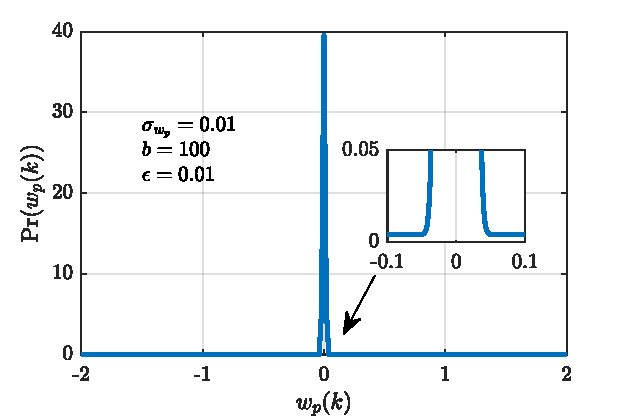
\includegraphics[width=11.5cm]{wpk-pdf-4.pdf}
	\caption{Probability density of a random shock signal}
	\label{fig:wpk-pdf}
\end{figure}

When dealing with a system having more than one \gls{RODD}, where each random shock is independent, the notation is
\begin{equation} \label{eq:wpik2}
	w_{p,i}(k) \sim 
	\begin{cases*}
		\mathcal{N}\left(0, \sigma_{w_p,i}^2\right) & with probability $1-\varepsilon_i$, \\
		\mathcal{N}\left(0, b_i^2\sigma_{w_p,i}^2\right) & with probability $\varepsilon_i$,
	\end{cases*}
\end{equation}
where $i \in \left\{1, 2, ..., n_p\right\}$.
\nomenclature{$n_p$}{number of independent random shock disturbance processes}%

The choice of $A(q^{-1})$ and $B(q^{-1})$ in \eqref{eq:RODD} determines the nature of the \gls{RODD}. For example, if $B(q^{-1})=1$ and $A(q^{-1})=1-q^{-1}$, $p(k)$ will be a random-walk process with infrequent, large step changes.

% Add symbol to glossary
Using $\nabla$ to denote $1-q^{-1}$, the \gls{RODD} \textit{step-disturbance} process can be defined as
\nomenclature{$\nabla$}{defined as $1-q^{-1}$}%
\begin{equation} \label{eq:RODD-step}
	p(k) = \frac{1}{\nabla}w_p(k).
\end{equation}

A \gls{RODD} \textit{ramp-disturbance}, consisting of a series of ramps with randomly-occurring changes in slope, may be generated using
\begin{equation} \label{eq:RODD-ramp}
	p(k) = \frac{1}{\nabla^2}w_p(k).
\end{equation}

A \gls{RODD} consisting of randomly-occurring decaying exponential changes may be generated using
\begin{equation} \label{eq:RODD-exp}
	p(k) = \frac{1}{(1-a_1q^{-1})\nabla}w_p(k),
\end{equation}
where  $0<a_1<1$. Note that $a_1=0$ corresponds to the case of a \gls{RODD} step disturbance \eqref{eq:RODD-step} and $a_1=1$ to that of a \gls{RODD} ramp disturbance \eqref{eq:RODD-ramp}. 

An equivalent state-space representation of \eqref{eq:RODD-exp} is
\begin{equation} \label{eq:RODD-ss}
	\begin{split}
		\mathbf{x}_p(k+1) & =\left[\begin{array}{cc}
			1 & 1 \\
			0 & a_1
		\end{array}\right] \mathbf{x}_p(k) +\left[\begin{array}{cc}
			0 \\
			1
		\end{array}\right] w_p(k) \\
		p(k) & =\left[\begin{array}{cc}
			1 & 0
		\end{array}\right] \mathbf{x}_p(k),
	\end{split}
\end{equation}
\nomenclature{$\mathbf{x}_p(k)$}{disturbance model states at time $k$}%
where $\mathbf{x}_p(k) \in \mathbb{R}^2$ is the state vector.

A disturbance with a combination of different \gls{RODD}s is also possible.  For example, a state-space representation of a \gls{RODD} consisting of step changes and ramps is
\begin{equation} \label{eq:RODD-step-ramp}
	\begin{split}
		\mathbf{x}_p(k+1) & =\left[\begin{array}{cc}
			1 & 1 \\
			0 & 1
		\end{array}\right] \mathbf{x}_p(k) +\left[\begin{array}{cc}
			1 & 0 \\
			0 & 1
		\end{array}\right] \mathbf{w}_p(k) \\
		p(k) & =\left[\begin{array}{cc}
			1 & 0
		\end{array}\right] \mathbf{x}_p(k),
	\end{split}
\end{equation}

where $\mathbf{w}_p(k)$ is a vector of two independent random shock signals generated by \eqref{eq:wpik2}. Simulated examples of these \gls{RODD}s are presented in figures \ref{fig:rodd-sim-plots} and \ref{fig:rodd-sim-plot2}.

\subsection{Hidden Markov models} \label{sec:HMM}

\textit{Hidden Markov models} (\gls{HMM}) can be used to simulate a more diverse set of switching behaviours than those of the \gls{RODD} model described in the previous section \citep{wong_realistic_2009}. A Markov process or Markov chain is a stochastic model used to describe a sequence of discrete events for which the probability of future events depends only on the current state. A \gls{HMM} is a Markov model with states that are not fully observable (i.e. hidden or observed with a measurement error).

To illustrate the basic concept, the state of the random shock process \eqref{eq:wpk2} \hl{may be defined} as a Markov model with a state that has two possible values,
\begin{equation} \label{eq:gamma-k}
	\gamma(k) \in \{0,1\}.
\end{equation}
\nomenclature{$\gamma(k)$}{random shock indicator at time $k$}%
$\gamma(k)=1$ represents a shock at time $k$, and $\gamma(k)=0$ means no shock occurs. The switching of $\gamma(k)$ can then be defined by a \textit{transition matrix}, $\Pi$, which describes the probabilities of transitioning from every mode at time $k$ to every mode at time $k+1$:
\begin{equation} \label{eq:Pi}
	\begin{aligned}
	\Pi &= \left(\pi_{ij} \forall i,j\in \{1,2,...,n_j\}\right) \\
	\pi_{ij} &= \Pr\left( \gamma(k)=j-1 \mid \gamma(k-1)=i-1 \right),
	\end{aligned}
\end{equation}
\nomenclature{$\Pr(A \mid B)$}{probability of an event $A$ given an event $B$}%
\nomenclature{$n_j$}{number of modes or models of a switching system}%
where $n_j$ is the number of possible system modes and $\pi_{ij}$ is the probability that the system mode at time $k$ is $j-1$ given that it was $i-1$ at time $k-1$.

In the case of the random shock, $n_j=2$ and the equivalent Markov process has the transition probability matrix
\nomenclature{$\Pi_{w_{p}}$}{transition probability matrix of the disturbance process $w_p$}%
\begin{equation} \label{eq:Pi-RODD-step}
	\Pi_{w_{p}} = \begin{bmatrix}
	1-\varepsilon & \varepsilon \\
	1-\varepsilon & \varepsilon
	\end{bmatrix}.
\end{equation}
Since $w_{p}(k)$ is an independent random variable, it does not depend on the previous state, $\gamma(k-1)$. Therefore, the rows of $\Pi_{w_{p}}$ are identical.

The use of the Markov model thus allows transition probabilities that do depend on the previous state. For example, consider a disturbance where the signal switches infrequently between samples from two or more distributions with different parameters. The probabilities of switching from one distribution to another may be different. Such a disturbance process could be simulated with a hidden Markov model by conditioning the distribution from which $w_p(k)$ is sampled on a Markov state, $r(k)$, with an arbitrary number of modes,
\nomenclature{$r(k)$}{mode indicator of a switching system at time $k$}%
\begin{equation} \label{eq:mog-example}
	\begin{split}
		w_p(k) \sim 
		\begin{cases*}
			\mathcal{N}\left(\mu_{w_p,1}, \sigma_{w_p,1}\right) & if $r(k)=1$, \\
			\mathcal{N}\left(\mu_{w_p,2}, \sigma_{w_p,2}\right) & if $r(k)=2$, \\
			... & ...\\
			\mathcal{N}\left(\mu_{w_p,n_j}, \sigma_{w_p,n_j}\right) & if $r(k)=n_j$.
		\end{cases*} \\
	\Pr(r(k)=j-1 \mid r(k-1)=i-1)=\pi_{ij} \forall i,j \in {1,2,...,n_j}
	\end{split}
\end{equation}

To make the notation more concise, allow the value of any time-varying discrete variable such as $\sigma_{w_p} \in \left\{\sigma_{w_p,1}, \sigma_{w_p,2},..., \sigma_{w_p,n_j}\right\}$, to be determined by the value of the Markov state $r(k)$. Thus,
\begin{equation} \label{eq:A-selection}
	\sigma_{w_p}(r(k)) = 
	\begin{cases*}
		\sigma_{w_p,1} & if $r(k)=1$, \\
		\sigma_{w_p,2} & if $r(k)=2$, \\
		... & ...\\
		\sigma_{w_p,n_j} & if $r(k)=n_j$.
	\end{cases*}
\end{equation}

With this notation, \eqref{eq:mog-example} can be written concisely as
\begin{equation} \label{eq:mog-example2}
	\begin{aligned}
		w_p(k) &\sim \mathcal{N}\left(\mu_{w_p}(r(k)), \sigma_{w_p}(r(k))\right) \\
		\Pr(r(k) &= j-1 \mid r(k-1)=i-1)=\pi_{ij} \forall i,j \in {1,2,...,n_j}.
	\end{aligned}
\end{equation}
where $\mu_{w_p}\in\left\{\mu_{w_p,1},\mu_{w_p,2},...,\mu_{w_p,n_j}\right\}$. This model is known as a \textit{mixture of Gaussians} and can be considered a special-case of a HMM-based disturbance model \citep{wong_disturbance_2007}.

A \gls{HMM} disturbance process can be represented by a \textit{Markov jump linear system} (\acrshort{MJLS}) \citep{costa_discrete-time_2005}. The state-space representation with time-varying system matrices $\mathbf{A}(\gamma(k))$, $\mathbf{B}(\gamma(k))$, and $\mathbf{C}(\gamma(k))$, and a vector of independent time-varying random shock inputs, $\mathbf{w}_p(k)$ \eqref{eq:mog-example2}, is defined
\begin{equation} \label{eq:MJLS}
	\begin{aligned}
	\mathbf{x}_p(k+1) &= \mathbf{A}(r(k)) \mathbf{x}_p(k) + \mathbf{B}(r(k))\mathbf{w}_p(k) \\
	\mathbf{p}(k) &= \mathbf{C}(r(k)) \mathbf{x}_p(k) + \mathbf{e}_p(k).
	\end{aligned}
\end{equation}

Note that $\mathbf{e}_p(k)$ may also be a switching random variable if desired. \eqref{eq:MJLS} is a versatile model suitable for representing and simulating a diverse family of stochastic disturbances.

\subsection{Bounded disturbances} \label{sec:bounded}

The \textit{bounded random walk} (\gls{BRW}) is a stochastic process proposed by \cite{nicolau_stationary_2002}. The discrete-time version is defined by the difference equation
\begin{equation} \label{eq:brw}
		p(k+1) = p(k) + a(p(k)) + e(k),
\end{equation}
where $e(k)$ is a random noise with variance $\sigma_e^2$, and $a(\cdot)$ is a function defined as
\nomenclature{$a(\cdot)$}{additive bias function used in the \acrshort{BRW}}%
\nomenclature{$\alpha_{1}$}{\acrshort{BRW} parameter}%
\nomenclature{$\alpha_{2}$}{\acrshort{BRW} parameter}%
\nomenclature{$\tau$}{\acrshort{BRW} parameter}%
\begin{equation}
	a(x) = e^{\beta}\left(e^{-\alpha_{1}\left(x - \tau\right)} - e^{\alpha_{2}\left(x - \tau\right)}\right),
\end{equation}
where $\beta$, $\alpha_{1}$, and $\alpha_{2}$ are constants.  From \eqref{eq:brw} it can be deduced that
\begin{equation}
	\mathbb{E}\{p(k+1)|p(k)\} = p(k) + a(p(k)).
\end{equation}

Therefore, $a(p(k))$ has the effect of an additive bias or time-varying adjustment to $p(k+1)$ that depends on $p(k)$. The shape of $a(\cdot)$ is determined by the constants $\alpha_{1}$,  $\alpha_{2}$, $\beta$, and $\tau$. Figure \ref{fig:brw-a} shows $a(p(k))$ in the case where $\tau=100$, $\beta=-15$, and $\alpha_{1}=\alpha_{2}=3$.  From this, it is clear that in the vicinity of $p(k)=\tau$, $a(p(k))\approx0$. When $a(p(k))=0$, \eqref{eq:brw} is the equation for a random walk. However, outside the neighbourhood, $p(k) \approx \tau$, $a(p(k))$ increases for low $p(k)$ or decreases for high $p(k)$. This has the effect of causing $p(k+1)$ to revert towards the mean ($\tau$) whenever $p(k)$ strays outside the neighbourhood. 
\begin{figure}[ht]
	\centering
	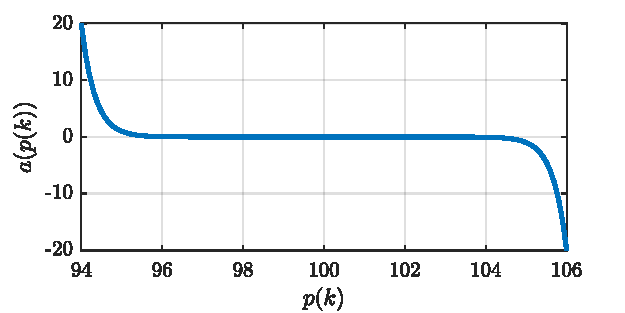
\includegraphics[height=5cm]{images/brw_a.pdf}
	\caption{A bounded random walk bias function}
	\label{fig:brw-a}
\end{figure}

Figure \ref{fig:brw-sim} shows a simulation of a \gls{BRW} with the above parameter values, and for comparison, an unbounded random walk (labelled `RW') generated with the same noise input. The dashed lines at $p(k)=95$ and $p(k)=105$ roughly indicate the location of the lower and upper bounds, which the \gls{BRW} only marginally exceeds.
\begin{figure}[ht]
	\centering
	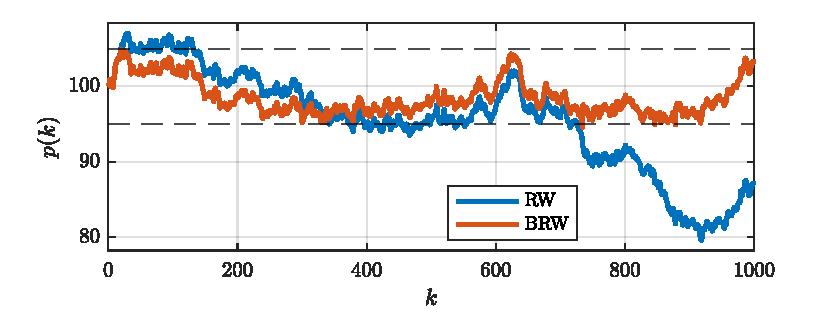
\includegraphics[height=5cm]{images/brw_sim.pdf}
	\caption{Examples of a bounded and unbounded random walk}
	\label{fig:brw-sim}
\end{figure}

Unlike a simple random walk, the \gls{BRW} is stationary. \cite{nicolau_stationary_2002} derived a formula for the form of the unconditional (i.e. stationary) probability distribution of the continuous-time \gls{BRW}. Figure \ref{fig:brw-pdf} shows the normalized stationary probability density of the \gls{BRW} defined above. For comparison, the probability density of a random walk process after 20 sample periods is also shown. It can be seen that there is a significant probability that the random walk would exceed the bounds of this \gls{BRW} after 20 sample periods. It can also be seen that the central part of the probability distribution of the \gls{BRW} is flat, indicating that all values within the bounds are equally likely after a large number of samples, similar to a uniform probability distribution.

%\begin{equation}
%	p_{BRW}(x) \propto \sigma^{-2} \exp \left\{-\frac{2 e^{k}}{\sigma^{2}}\left(\frac{e^{-\alpha_{1}(x-\tau)}}{\alpha_{1}}+\frac{e^{\alpha_{2}(x-\tau)}}{\alpha_{2}}\right)\right\}
%\end{equation}

\begin{figure}[ht]
	\centering
	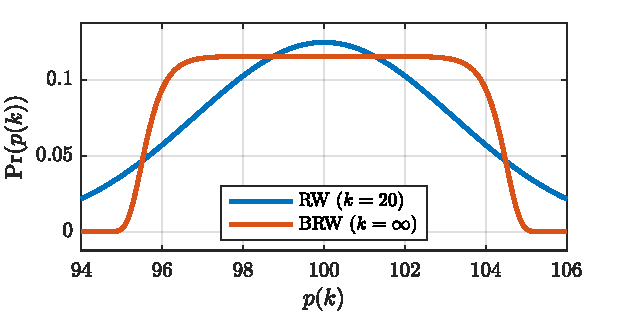
\includegraphics[height=5cm]{images/brw_pdf.pdf}
	\caption{Probability distributions of bounded and unbounded random walks}
	\label{fig:brw-pdf}
\end{figure}

However, the \gls{BRW} as defined in \eqref{eq:brw} is not guaranteed to be stable. Extreme values of $p(k)$ may cause $|a(p(k))|$ to be greater than $2|p(k)|$, which results in rapid divergence. This would cause computational errors in a numerical simulation. To avoid this, \cite{nicolau_stationary_2002} recommends adding a conditional regularizing step that forces reversion towards the mean, $\tau$, when the correction bias is too large. Instead of \eqref{eq:brw}, a conditional difference equation,
\begin{equation} \label{eq:brw-reg}
	p(k+1) = \begin{cases*}
		p(k) + a(p(k)) + e(k) & if $\left|a(p(k)) \right| < 2\left| p(k) - \tau \right|$, \\
		\tau + \phi(p(k) - \tau) + e(k) & if $\left|a(p(k)) \right| \geq 2\left| p(k) - \tau \right|$,
	\end{cases*}
\end{equation}
is used, where $\phi$ is a constant such that $0<\phi<1$. The size of $\phi$ determines how fast $p(k)$ reverts to $\tau$ when it is outside the stable region.

Since the \gls{BRW} has a non-Gaussian probability distribution, analysis of the properties of any dynamical system with a \gls{BRW} input is difficult. However, for simulation purposes, the \gls{BRW} is a simple and practical solution to the problem of bounding a random disturbance.

The \gls{BRW} concept could be extended to \gls{RODD}s. A \gls{RODD} step disturbance \eqref{eq:RODD-step} is a random walk with a switching noise variance \eqref{eq:wpk2}. The concern when trying to bound such a disturbance is the large step changes that occur infrequently. Since the probability of the shock, as well as the sign and amplitude of the step, are independent random variables, a \gls{RODD} step disturbance that happens to be at one of the bounds is as likely to step outside the bound as it is to step back inside the bounded region. The conditional regularity used in the \gls{BRW} \eqref{eq:brw-reg} would prevent any computational problems.


\section{State estimation} \label{sec:estimation}

State estimation is the task of estimating the values of the state variables of a dynamic model of a system given a set of measurements from the system. In process control applications, estimates of the states at the current time, or a prediction of their values at the next time instant, are required in real time (i.e. online) in order to calculate an appropriate control action.

Consider the diagram of an input-output system model in Figure \ref{fig:model_diag_uwvy}. Here, $\mathbf{u}(k)$ $\in \mathbb{R}^{n_u}$ is a vector of known input variables at time instant $k$, $\mathbf{w}(k)$ $\in \mathbb{R}^n$ is a vector of unmeasured state disturbances, $\mathbf{v}(k) \in \mathbb{R}^{n_y}$ is a vector of measurement errors, and $\mathbf{y}_M(k) \in \mathbb{R}^{n_y}$ is a vector of output measurements. The box represents a mathematical model that relates the inputs to the outputs and may be time-varying.
\nomenclature{$\mathbf{u}(k)$}{system inputs at time $k$}%
\nomenclature{$\mathbf{y}(k)$}{system outputs at time $k$}%
\nomenclature{$\mathbf{w}(k)$}{process disturbances at time $k$}%
\nomenclature{$\mathbf{v}(k)$}{measurement noises at time $k$}%
\begin{figure}[ht]
	\centering
	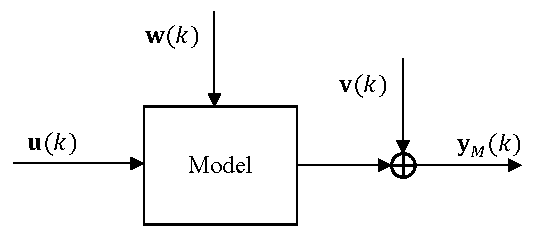
\includegraphics[width=8cm]{images/model_diag_uwvy.pdf}
	\caption{System model diagram}
	\label{fig:model_diag_uwvy}
\end{figure}

A convenient form in which to represent discrete-time, linear, possibly time-varying, dynamical system models for state estimation and control purposes, is the state-space representation
\begin{equation} \label{eq:ss_rep_uwy}
	\begin{aligned}
		\mathbf{x}(k+1) &= \mathbf{A}(k) \mathbf{x}(k) + \mathbf{B}(k) \mathbf{u}(k) + \mathbf{w}(k), \\
		\mathbf{y}_M(k) &= \mathbf{C}(k) \mathbf{x}(k) + \mathbf{v}(k).
	\end{aligned}
\end{equation}
\nomenclature{$\mathbf{x}(k)$}{system model states at time $k$}%
\nomenclature{$\mathbf{A}$}{transition matrix of the system model}%
\nomenclature{$\mathbf{B}$}{input matrix of the system model}%
\nomenclature{$\mathbf{C}$}{output matrix of the system model}%
where $\mathbf{x}(k)$ $\in \mathbb{R}^n$ is a vector of state variables, $\mathbf{A}(k) \in \mathbb{R}^{n \times n}$ is the state transition matrix at time $k$, $\mathbf{B}(k) \in \mathbb{R}^{n \times n_u}$ is the input matrix at time $k$, and $\mathbf{C}(k) \in \mathbb{R}^{n_y \times n}$ is the output matrix at time $k$. In this work, the system matrices are not time-varying and are therefore denoted $\mathbf{A}$, $\mathbf{B}$, and $\mathbf{C}$ in the remainder of this chapter.

The \textit{Kalman filter} \citep{kalman_new_1960} is the optimal estimator for a linear system in which the unmeasured disturbances and measurement errors are Gaussian random variables with mean values of zero. There are two commonly-used implementations of the Kalman filter, the \textit{prediction form} and the \textit{filtering form}. In the prediction form, the estimates of the states at the next time instant ($k+1$), given the information available at the current time ($k$) are calculated using
\begin{equation}
\begin{aligned} \label{eq:xkp1_hat_p}
	\mathbf{\hat{x}}(k+1 \mid k) &= \mathbf{\hat{x}}(k+1 \mid k-1) + \mathbf{K}_p(k) \big( \mathbf{y}_M(k) - \mathbf{\hat{y}}(k \mid k-1) \big) \\
	&= \mathbf{A}\mathbf{\hat{x}}(k \mid k-1) + \mathbf{B}\mathbf{u}(k) + \mathbf{K}_p(k) \big( \mathbf{y}_M(k) - \mathbf{C} \mathbf{\hat{x}}(k \mid k-1) \big)
\end{aligned}
\end{equation}
\nomenclature{$\mathbf{y}_M(k)$}{system output measurements at time $k$}%
where $\hat{\mathbf{x}}(k \mid k-1)$ is the prediction of the states at time $k$ that was made with the information available at the previous time instant, $k-1$, $\mathbf{y}_M(k)$ is the current measurement of the output, and $\mathbf{K}_p(k) \in \mathbb{R}^{n \times n_y}$ is a (possibly time-varying) correction gain.
\nomenclature{$\mathbf{K}_p(k)$}{correction gain of the Kalman filter (prediction form)}%

In the filtering form, which is used in this work, the estimated states and outputs at the current time are calculated given the information available at the current time using
\begin{equation} \label{eq:xkyk_hat}
	\begin{aligned}
		\mathbf{\hat{y}}(k \mid k-1) &= \mathbf{C} \mathbf{\hat{x}}(k \mid k-1) \\
		\mathbf{\hat{x}}(k \mid k) &= \mathbf{\hat{x}}(k \mid k-1) + \mathbf{K}(k) \big( \mathbf{y}_M(k) - \mathbf{\hat{y}}(k \mid k-1)  \big) \\
		\mathbf{\hat{y}}(k \mid k) &= \mathbf{C} \mathbf{\hat{x}}(k \mid k)
	\end{aligned}
\end{equation}
\nomenclature{$\hat{\mathbf{x}}(k \mid k-1)$}{predictions of system model states at time $k$ made with information available at time $k-1$}%
\nomenclature{$\mathbf{K}(k)$}{correction gain of the Kalman filter (filtering form)}%
where $\mathbf{K}(k)$ $\in \mathbb{R}^{n \times n_y}$ is a (possibly time-varying) correction gain. Instead of \eqref{eq:xkp1_hat_p}, the predictions of the states at the next time instant are calculated using
\nomenclature{$\hat{\mathbf{x}}(k+1 \mid k)$}{predictions of system modelstates at time $k+1$ made with information available at time $k$}%
\nomenclature{$\hat{\mathbf{x}}(k \mid k)$}{estimates of system model states at time $k$ made with information available at time $k$}%
\nomenclature{$\hat{\mathbf{y}}(k \mid k)$}{estimates of system outputs at time $k$ made with information available at time $k$}%
\begin{equation} \label{eq:xkp1_hat}
	\mathbf{\hat{x}}(k+1 \mid k) = \mathbf{A} \mathbf{\hat{x}}(k \mid k) + \mathbf{B} \mathbf{u}(k).
\end{equation}

An intuitive interpretation of the Kalman filter is that it takes the predictions of the states at time $k$ made in the previous time instant using the system model, and corrects them based on the difference between the current output measurement, $\mathbf{y}_M(k)$, and the output predicted by the model, $\mathbf{C} \mathbf{\hat{x}}(k \mid k-1)$. The correction step \eqref{eq:xkyk_hat} and prediction step \eqref{eq:xkp1_hat} are executed iteratively each time step, given a prior prediction of the states at time zero, $\mathbf{\hat{x}}(0 \mid -1)=\mathbf{\hat{x}}_0$.
\nomenclature{$\mathbf{\hat{x}}_0$}{Initial values of the estimates of the system states at time 0}%

Although the predicted states, $\hat{\mathbf{x}}(k \mid k-1)$, are identical in both forms of the Kalman filter, the use of the updated (i.e. \textit{a posteriori}) estimates, $\hat{\mathbf{x}}(k \mid k)$, in the filtering form instead of the predicted states leads to an optimal estimate taking account of all the information available. However, it should be noted that in some control applications, the prediction form is beneficial because the state predictions, $\hat{\mathbf{x}}(k+1 \mid k)$, are available one time step ahead.

To track a system with time-varying parameters, a dynamic estimator is needed with a time-varying correction gain. In the case of the filtering form of the Kalman filter, $\mathbf{K}(k)$ is calculated at each time instant using
\begin{equation} \label{eq:Kk}
	\mathbf{K}(k) = \mathbf{P}(k \mid k-1)\mathbf{C}^\intercal \mathbf{S}^{-1}(k),
\end{equation}
where $\mathbf{S}(k)$ is the output prediction error covariance matrix, which is given by
\nomenclature{$\mathbf{S}(k)$}{covariance of the output prediction errors at time $k$}%
\begin{equation} \label{eq:Sk}
	\mathbf{S}(k) = \mathbf{C}\mathbf{P}(k \mid k-1)\mathbf{C}^\intercal + \mathbf{R},
\end{equation}
\nomenclature{$\mathbf{P}(k \mid k-1)$}{predictions of the state estimation error covariance at time $k$ made with information available at time $k-1$}%
and $\mathbf{P}(k \mid k-1)$ is the state estimation error covariance matrix calculated in the previous time instant. $\mathbf{R}$, which is time invariant in this work, is the covariance matrix of the measurement noises,
\nomenclature{$\mathbf{R}$}{covariance of the measurement noises in the observer model}%
\begin{equation} \label{eq:R}
	 \mathbf{R} = \mathbb{E}\{ \mathbf{v}(k) \mathbf{v}^\intercal(k) \},
\end{equation}
\nomenclature{$\mathbb{E}\{\cdot\}$}{expectation operator}%
where $\mathbb{E}\{\cdot\}$ is the expectation operator.

The corrected error covariance may be calculated using
\nomenclature{$\mathbf{P}(k \mid k)$}{state estimation error covariance at time $k$ made with information available at time $k$}%
\begin{equation} \label{eq:Pk}
	\mathbf{P}(k \mid k) = \left( \mathbf{I}_n - \mathbf{K}(k) \mathbf{C} \right) \mathbf{P}(k \mid k-1),
\end{equation}
given an initial covariance estimate at time zero, $\mathbf{P}(0 \mid -1)=\mathbf{P}_0$.%
\nomenclature{$\mathbf{P}_0$}{Initial value of the state estimation error covariance at time 0}

However, to reduce numerical errors due to rounding, the computation of $\mathbf{P}(k \mid k)$ is carried out in this work using the Joseph stabilized version of \eqref{eq:Pk} {\citep{lewis_optimal_2008}
 \begin{equation} \label{eq:Pk-stab}
 	\mathbf{P}(k \mid k) = \left( \mathbf{I}_n - \mathbf{K}(k) \mathbf{C} \right ) \mathbf{P}(k \mid k-1) \left( \mathbf{I}_n - \mathbf{K}(k) \mathbf{C} \right )^\intercal + \mathbf{K}(k)  \mathbf{R} \mathbf{K}(k)^\intercal,
 \end{equation}
\nomenclature{$\mathbf{I}_n$}{the identity matrix ($n \times n$)}%
where $\mathbf{I}_n$ is the identity matrix.

The prediction of the error covariance at the next time instant is made using
\nomenclature{$\mathbf{P}(k+1 \mid k)$}{predictions of the state estimation error covariance at time $k+1$ made with information available at time $k$}%
\begin{equation} \label{eq:Pkp1}
	\mathbf{P}(k+1 \mid k) = \mathbf{A} \mathbf{P}(k \mid k)  \mathbf{A}^\intercal  + \mathbf{Q}(k),
\end{equation}
where $\mathbf{Q}(k)$ is the time-varying covariance of the process disturbances,
\nomenclature{$\mathbf{Q}(k)$}{covariance of the process disturbances in the observer model at time $k$}%
\begin{equation} \label{eq:Q}
	\mathbf{Q}(k) = \mathbb{E}\{ \mathbf{w}(k) \mathbf{w}^\intercal(k) \}.
\end{equation}

Algorithm \ref{alg:kf} defines the sequence of the Kalman filter calculations at each time instant. 
\nomenclature{$\mathcal{Q}$}{set of process noise covariance matrices of a switching system model}%
This is for the case with only the covariance, $\mathbf{Q}(k)$, switching according to the shock indicator, $\gamma(k)$, \eqref{eq:init_Q}. It can easily be extended to simulate other switching model components, such as $\mathbf{R}(k)$, $\mathbf{A}(k)$, $\mathbf{B}(k)$, or $\mathbf{C}(k)$ as defined in \eqref{eq:ss_rep_uwy}. \hl{An alternative to the representation used in this work would be to implement the switching of the random shock {\eqref{eq:wpk2}} using a time-varying input matrix, $\mathbf{B}(k)$, instead of the time-varying prediction error covariance, $\mathbf{Q}(k)$ in {\eqref{eq:Pkp1}}. Both methods are valid and equivalent.}
\begin{algorithm}
	\caption{Kalman filter update}\label{alg:kf}
	%\algorithmfootnote{$y_0$ denotes the initial value.}
	\begin{algorithmic}
		\Require $\mathbf{A},\mathbf{B},\mathbf{C},\mathbf{\hat{x}}(k \mid k-1), \mathbf{P}(k \mid k-1), \mathcal{Q}, \mathbf{R}, \mathbf{\gamma}(k), \mathbf{u}(k), \mathbf{y}_M(k)$
		\State calculate $\mathbf{S}(k)$ \eqref{eq:Sk}
		\State calculate $\mathbf{K}(k)$ \eqref{eq:Kk}
		\State calculate $\mathbf{\hat{x}}(k \mid k)$ and $\mathbf{\hat{y}}(k \mid k)$ \eqref{eq:xkyk_hat}
		\State calculate $\mathbf{P}(k \mid k)$ \eqref{eq:Pk-stab}
		\State calculate $\mathbf{\hat{x}}(k+1 \mid k)$ \eqref{eq:xkp1_hat}
		\State $\mathbf{Q}(k) \gets \mathcal{Q}(\gamma(k))$
		\State calculate $\mathbf{P}(k+1 \mid k)$ \eqref{eq:Pkp1}
	\end{algorithmic}
\end{algorithm}

Also note that in a control application, the manipulated input, $\mathbf{u}(k)$, is computed by the control algorithm. This may be done before the Kalman filter calculations in algorithm \ref{alg:kf} if the prior prediction of the states in the current time instant, $\hat{\mathbf{x}}(k \mid k-1)$, is used. Alternatively, slightly better control performance might be achieved if the control algorithm uses the updated (a-posteriori) state estimates, $\hat{\mathbf{x}}(k \mid k)$. In the latter case, the Kalman filter calculations must be interrupted to compute the control action after the state correction step \eqref{eq:xkyk_hat} and prior to the prediction step \eqref{eq:xkp1_hat}, when $\mathbf{u}(k)$ is needed.

\begin{figure}[ht]
	\centering
	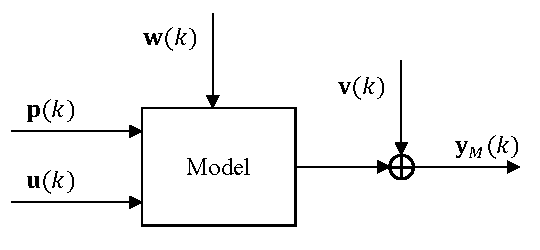
\includegraphics[width=8cm]{images/model_diag_upwvy.pdf}
	\caption{System model with disturbance inputs and manipulated inputs}
	\label{fig:model_diag_upwvy}
\end{figure}
In the case where the system has unmeasured disturbance inputs, $\mathbf{p}(k) \in \mathbb{R}^{n_p}$, as depicted in Figure \ref{fig:model_diag_upwvy}, the state-space equations \eqref{eq:ss_rep_uwy} are modified to include these by splitting the input matrix into two parts, $\mathbf{B}_u \in \mathbb{R}^{n \times n_u}$ and $\mathbf{B}_p \in \mathbb{R}^{n \times n_p}$,
\begin{equation} \label{eq:ss_rep_upwy}
	\begin{aligned}
		\mathbf{x}(k+1) = \mathbf{A} \mathbf{x}(k) + \mathbf{B}_u \mathbf{u}(k) + \mathbf{B}_p \mathbf{p}(k) + \mathbf{w}(k), \\
		\mathbf{y}_M(k) = \mathbf{C} \mathbf{x}(k) + \mathbf{v}(k).
	\end{aligned}
\end{equation}

For state estimation in the presence of unmeasured disturbances, which is always the case in practice, a suitable model of the disturbances is needed. This model is shown in Figure \ref{fig:model_diag_wpupwvy} with a vector of random shock variables, $\mathbf{w}_p(k)$, at its input.
\nomenclature{$\mathbf{w}_p(k)$}{random shock signals at time $k$}%
\begin{figure}[ht]
	\centering
	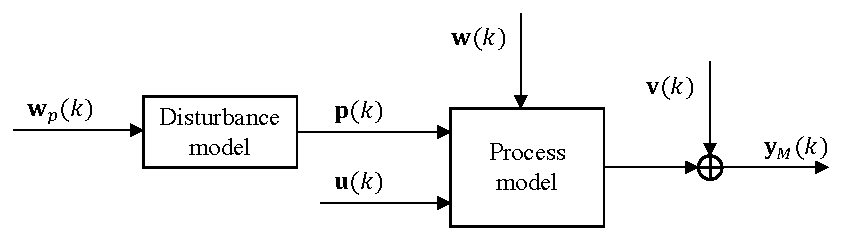
\includegraphics[width=12.5cm]{images/model_diag_wpupwvy.pdf}
	\caption{System with process model and disturbance model}
	\label{fig:model_diag_wpupwvy}
\end{figure}

A state-space representation of the combined system including the disturbance model can be constructed. This is referred to as the \textit{augmented system model},
\begin{equation} \label{eq:ss_rep_xa}
	\begin{aligned}
		\mathbf{x}_a(k+1) = \mathbf{A}_a \mathbf{x}_a(k) + \mathbf{B}_{a,u} \mathbf{u}(k) + \mathbf{B}_{a,w} \mathbf{w}_{a}(k), \\
		\mathbf{y}(k) = \mathbf{C}_a \mathbf{x}_a(k) + \mathbf{v}(k),
	\end{aligned}
\end{equation}
%\nomenclature{$\mathbf{x}_a(k)$}{augmented system states at time $k$}%
where $\mathbf{x}_a(k) \in \mathbb{R}^{n+n_p}$ is an augmented state vector that includes the states of both the process model and the disturbance model, 
\begin{equation} \label{eq:xak}
	\mathbf{x}_a(k) = \begin{bmatrix}
		\mathbf{x}(k) \\
		\mathbf{x}_p(k)
	\end{bmatrix},
\end{equation}
and $\mathbf{w}_a(k) \in \mathbb{R}^{n+n_p}$ is an augmented vector of random variables, including the random shocks,
\begin{equation} \label{eq:wak}
	\mathbf{w}_a(k) = \begin{bmatrix}
		\mathbf{w}(k) \\
		\mathbf{w}_p(k)
	\end{bmatrix}.
\end{equation}

However, note that this notation with subscript `a' is only used in this section. In subsequent sections, the subscript is dropped for simplicity since all references to the system model refer to the augmented model used for state estimation.

Although the random shock in a \gls{RODD} is unmeasured, it may be observable from the measurements of the outputs of the system. As mentioned in Section \ref{detection_RODDs}, systems with \gls{RODD}s pose problems for state estimation using standard Kalman filters due to the switching of the noise model parameters, namely, the variance of $w_p(k)$ \eqref{eq:wpk2}. As explained by \cite{andersson_adaptive_1985}, a trade-off must be made during the filter design between its ability to respond to the infrequent disturbance when it occurs, and its sensitivity to noise at other times.


\subsection{Multiple model approaches} \label{sec:multi-model}

One option for state estimation of switching (i.e. hybrid) systems is the so-called \textit{multiple-model approach}. Multiple-model observers account for different possible hypotheses about the current and past states of the system and infer from these an overall `best' estimate of the current states. To achieve this, an independent Kalman filter is maintained for each hypothesis and a weighted average of the estimates by each filter is calculated using the conditional probabilities of each hypothesis given current and past measurements.

Let the number of hypotheses and Kalman filters be $n_h$ and the \textit{shock mode hypothesis} associated with Kalman filter $f$ at time $k$ be
\nomenclature{$n_h$}{number of hypotheses maintained by a multiple-model observer}%
\begin{equation} \label{eq:gammak}
	\gamma_{f}(k) \in \left\{0, 1 \right\} \forall{k \ge 0}.
\end{equation}

First, consider the case of estimating only one shock signal \eqref{eq:wpk2}. Therefore, $\gamma_f(k)$ is a scalar. The transition probabilities of the random shock are independent of previous shocks:
\nomenclature{$\gamma_f(k)$}{random shock indicator of hypothesis $f$ at time $k$}%
\begin{equation} \label{eq:Pr_gammak_given_gammakm1}
	\begin{aligned}
		& \Pr\left(\gamma_{f}(k)=0 \mid \gamma_{f}(k-1)\right) = \Pr\left(\gamma_{f}(k)=0\right) = 1-\varepsilon, \\
		& \Pr\left(\gamma_{f}(k)=1 \mid \gamma_{f}(k-1)\right) = \Pr\left(\gamma_{f}(k)=1\right) = \varepsilon.
	\end{aligned}
\end{equation}

After $k$ time steps, the complete shock mode hypothesis sequence associated with filter $f$ is
\nomenclature{$\Gamma_f(k)$}{shock indicator hypotheses sequence $f$ from time $0$ to $k$}%
\begin{equation} \label{eq:Gammak}
	\Gamma_f(k) = \left\{ \gamma_f(0), \gamma_f(1), ..., \gamma_f(k) \right\}.
\end{equation}

The known system inputs and output measurements up to time $k$ are
\nomenclature{$\mathbf{U}(k)$}{known system inputs from time 0 to time $k$}%
\nomenclature{$\mathbf{Y}(k)$}{system outputs from time 0 to time $k$}%
\nomenclature{$\mathbf{Y}_M(k)$}{system output measurements from time 0 to time $k$}%
\begin{equation} \label{eq:Uk_Yk}
	\begin{aligned}
		\mathbf{U}(k) = \left\{ \mathbf{u}(0), \mathbf{u}(1), ..., \mathbf{u}(k) \right\} \\
		\mathbf{Y}_M(k) = \left\{ \mathbf{y}_M(0), \mathbf{y}_M(1), ..., \mathbf{y}_M(k) \right\}.
	\end{aligned}
\end{equation}

Assume that new measurements are made available at each time $k$. The probability of the shock hypothesis sequences associated with each filter given the data up to time $k$ can be calculated recursively using the following equations. At time $k$, the probability of the shock hypothesis sequence associated with filter $f$ given the data up to time $k-1$ is
\begin{multline} \label{eq:Pr_Gammak_given_Ykm1}
	\Pr(\Gamma_f(k) \mid \mathbf{Y}_M(k-1)) = 
	\Pr(\gamma_f(k) \mid \gamma_f(k-1)) \Pr(\Gamma_f(k-1) \mid \mathbf{Y}_M(k-1)).
\end{multline}

The conditional probability densities of the measurements, $\mathbf{y}_M(k)$, are approximated by Gaussian distributions centred on the output predictions, $\mathbf{\hat{y}}_{f}(k \mid k-1)$,  and with the variance of the output prediction error, $\mathbf{S}_f(k)$,
\begin{equation} \label{eq:p_yk_given_Gammak_Ykm1}
	p(\mathbf{y}_M(k) \mid \Gamma_f(k), \mathbf{Y}_M(k-1)) \approx \mathcal{N}\left(\mathbf{y}_M(k), \mathbf{\hat{y}}_{f}(k \mid k-1),	\mathbf{S}_f(k) \right)
\end{equation}
\nomenclature{$\mathcal{N}(\mathbf{y}, \mathbf{\mu}, \Sigma)$}{multivariate normal probability density of $\mathbf{y}$ with mean $\mathbf{\mu}$ and covariance $\Sigma$}%
where $p(\cdot)$ here represents a probability density function and $\mathcal{N}(\mathbf{y}, \mathbf{\mu}, \Sigma)$ denotes the multivariate normal probability density of $\mathbf{y}$ with mean $\mathbf{\mu}$ and variance $\Sigma$. $\mathbf{\hat{y}}_{f}(k \mid k-1)$ and $\mathbf{S}_f(k)$ are calculated as $\mathbf{\hat{y}}(k \mid k-1)$ and $\mathbf{S}(k)$ for a single Kalman filter, using 
\begin{equation} \label{eq:yfk_pred}
	\mathbf{\hat{y}}_{f}(k \mid k-1) = \mathbf{C}\mathbf{\hat{x}}_{f}(k \mid k-1)
\end{equation}
and
\nomenclature{$\mathbf{S}_f(k)$}{covariance of the output prediction errors of Kalman filter $f$ at time $k$}%
\begin{equation} \label{eq:Sfk}
	\mathbf{S}_f(k) = \mathbf{C}\mathbf{P}_f(k \mid k-1)\mathbf{C}^\intercal + \mathbf{R},
\end{equation}
where $\mathbf{\hat{x}}_{f}(k \mid k-1)$ and $\mathbf{P}_f(k \mid k-1)$ are the state predictions and prediction error covariances of Kalman filter $f$ calculated in the previous time step.

Finally, the estimate of the probability of shock hypothesis sequence $\Gamma_f(k)$ given the data up to time $k$ is
\begin{equation} \label{eq:Pr_Gammak_given_Yk}
	\Pr(\Gamma_f(k) \mid \mathbf{Y}_M(k)) = \frac{q_f(k)}{\sum_{f=1}^{n_h} q_f(k)},
\end{equation}
where
\begin{equation} \label{eq:qfk}
	q_f(k) = p(\mathbf{y}_M(k) \mid \Gamma_f(k), \mathbf{Y}_M(k-1)) \Pr(\Gamma_f(k) \mid \mathbf{Y}_M(k-1)).
\end{equation}

The Kalman filters for tracking each hypothesis use the state-space representation of the augmented system model \eqref{eq:ss_rep_xa}. Since the system includes a \gls{RODD} with a switching noise variance, it is a \textit{hybrid dynamical system} (refer to Section \ref{sec:lit-hybrid}). Define the set of possible covariance matrices of this system as
\begin{equation} \label{eq:init_Q_R}
	\mathcal{Q} = \left\{\mathbf{Q}_0, \mathbf{Q}_1\right\},
\end{equation}
and, for convenient notation, let $\mathcal{Q}$ be indexed by the shock indicator $\gamma_f(k)$,
\begin{equation} \label{eq:init_Q}
	\mathcal{Q}(\gamma_f(k)) = 
	\begin{cases*}
		\mathbf{Q}_0 & \text{if} $\gamma_f(k)=0$, \\
		\mathbf{Q}_1 & \text{if} $\gamma_f(k)=1$.
	\end{cases*}
\end{equation}

At the start of a simulation, $f$ Kalman filters are initialized with initial state estimates, $\mathbf{\hat{x}}_f(0) = \mathbf{\hat{x}}_{f,0}$, and initial error covariance estimates $	\mathbf{P}_f(0) = \mathbf{P}_{f,0}$. At each time instant, starting at $k=0$, the correction gains are calculated as in the previous section \eqref{eq:Kk},
\nomenclature{$\mathbf{K}_f(k)$}{correction gain (filtering form) of Kalman filter $f$}%
\begin{equation} \label{eq:Kfk}
	\mathbf{K}_f(k) = \mathbf{P}_f(k \mid k-1)\mathbf{C}^\intercal \mathbf{S}_f^{-1}(k).
\end{equation}

The corrected state and output estimates are calculated as in \eqref{eq:xkyk_hat}, given the current measurement using
\nomenclature{$\mathbf{\hat{x}}_f(k \mid k)$}{estimates of the system states at time $k$ for hypothesis $f$}%
\nomenclature{$\mathbf{\hat{y}}_f(k \mid k)$}{estimates of the system outputs at time $k$ for hypothesis $f$}%
\begin{equation} \label{eq:xfkyfk_hat}
	\begin{aligned}
		\mathbf{\hat{x}}_f(k \mid k) &= \mathbf{\hat{x}}_f(k \mid k-1) + \mathbf{K}_f(k) \big( \mathbf{y}_M(k) - \mathbf{C} \mathbf{\hat{x}}_f(k \mid k-1) \big) \\
		\mathbf{\hat{y}}_f(k \mid k) &= \mathbf{C} \mathbf{\hat{x}}_f(k \mid k).
	\end{aligned}
\end{equation}

The corrected error covariances are calculated as in \eqref{eq:Pk-stab} using 
\nomenclature{$\mathbf{P}_f(k \mid k)$}{state estimation error covariance of filter $f$ at time $k$ made with information available at time $k$}%
\nomenclature{$\mathbf{P}_f(k \mid k-1)$}{predictions of the state estimation error covariance of filter $f$ at time $k$ made with information available at time $k-1$}%
\begin{equation} \label{eq:Pkf-stab}
	\mathbf{P}_f(k \mid k) = \left( \mathbf{I}_n - \mathbf{K}_f(k) \mathbf{C} \right ) \mathbf{P}_f(k \mid k-1) \left( \mathbf{I}_n - \mathbf{K}_f(k) \mathbf{C} \right )^\intercal + \mathbf{K}_f(k) \mathbf{R} \mathbf{K}_f(k)^\intercal.
\end{equation}

An additional precaution is necessary here for numerical stability. $\mathbf{P}_f(k \mid k)$ should always be positive definite. However, because finite floating-point representations are inexact, it may potentially loose its positive definiteness. If this occurs, then $\mathbf{S}_f(k)$ will also not be positive definite, and a numerical error is likely when calculating the probability density of the output estimates \eqref{eq:p_yk_given_Gammak_Ykm1}. To avoid this problem the following operation is carried out after \eqref{eq:Pkf-stab}
\begin{equation} \label{eq:Pkf-psd-fix}
	\mathbf{P}_f(k \mid k) \gets \frac{ \mathbf{P}_f(k \mid k) + \mathbf{P}_f(k \mid k)^\intercal )}{2}. 
\end{equation}

This ensures that $\mathbf{P}_f(k \mid k)$ is always positive definite.

The predicted states at the next time instant are calculated as in \eqref{eq:xkp1_hat}
\begin{equation} \label{eq:xfkp1_hat}
	\mathbf{\hat{x}}_f(k+1 \mid k) = \mathbf{A} \mathbf{\hat{x}}_f(k \mid k) + \mathbf{B} \mathbf{u}(k)
\end{equation}
and the predicted error covariances at the next time instant are calculated as in \eqref{eq:Pkp1} using
\nomenclature{$\mathbf{P}_f(k+1 \mid k)$}{predictions of the state estimation error covariance of filter $f$ at time $k+1$ made with information available at time $k$}%
\begin{equation} \label{eq:Pfkp1}
	\mathbf{P}_f(k+1 \mid k) = \mathbf{A} \mathbf{P}_f(k \mid k)  \mathbf{A}^\intercal  + \mathcal{Q}(\gamma_f(k)).
\end{equation}

Note the difference between \eqref{eq:Pfkp1} and \eqref{eq:Pkp1}.  Here, $\mathbf{P}_f(k+1 \mid k)$ is dependent on $\gamma_f(k)$, which determines the noise covariance matrix used in the update, whereas in \eqref{eq:Pkp1}, $\mathbf{Q}$ is time invariant.

Finally, the merged estimates of the states and outputs at the current time are the sum of the Kalman filter estimates weighted by the conditional probabilities from \eqref{eq:Pr_Gammak_given_Yk},
\begin{equation} \label{eq:xkyk_hat_MKF}
	\begin{aligned}
		\mathbf{\hat{x}}(k \mid k) = \sum_{f=1}^{n_h} \mathbf{\hat{x}}_f(k \mid k) \Pr(\Gamma_f(k) \mid \mathbf{Y}_M(k)) \\
		\mathbf{\hat{y}}(k \mid k) = \sum_{f=1}^{n_h} \mathbf{\hat{y}}_f(k \mid k) \Pr(\Gamma_f(k) \mid \mathbf{Y}_M(k)).
	\end{aligned}
\end{equation}

A merged estimate of the covariance of the estimation errors is obtained using
\begin{equation} \label{eq:Pk_MKF}
	\begin{aligned}
	\mathbf{P}(k \mid k) = \sum_{f=1}^{n_h} \Pr(\Gamma_f(k) \mid \mathbf{Y}_M(k)) \left( \mathbf{P}_f(k \mid k) + \delta_\mathbf{\hat{x}}(k) \delta_\mathbf{\hat{x}}^\intercal(k) \right), \\
	\delta_\mathbf{\hat{x}}(k) = \mathbf{\hat{x}}(k \mid k) - \mathbf{\hat{x}}_f(k \mid k).
	\end{aligned}
\end{equation}

Algorithm \ref{alg:afmm} shows the sequence of operations and flow control loops to execute these computations during a simulation of length $N$ time steps.
\nomenclature{$N$}{length of a simulation in number of sampling intervals}%
\begin{algorithm}
	\caption{Multiple model observer simulation}  \label{alg:afmm}
	%\algorithmfootnote{$y_0$ denotes the initial value.}
	\begin{algorithmic}
			\Require $\mathbf{A}, \mathbf{B}, \mathbf{C}, \mathbf{\hat{x}}_0, \mathbf{\gamma}_{\text{init}}, \mathbf{p}_{\text{init}}, \mathbf{P}_0, \mathcal{Q}, \mathbf{R}, \Pi, \mathbf{U}(N), \mathbf{Y}_M(N)$
			\For{$f \gets 1, n_h$}  \Comment{Initialize Kalman filters}  % \footnotemark
				\State $\mathbf{\hat{x}}_f(0 \mid -1) \gets \mathbf{\hat{x}}_0$
				\State $\mathbf{P}_f(0 \mid -1) \gets \mathbf{P}_0$
				\State $\mathbf{\gamma}_f(-1) \gets \mathbf{\gamma}_{\text{init},f}$
				\State $\Pr(\Gamma_f(-1)|\mathbf{Y}_M(-1))) \gets p_{\text{init},f}$
			\EndFor
			\For{$k \gets 0, N$}
			\For{$f \gets 1, n_h$}
				\State calculate $\mathbf{\hat{y}}_f(k \mid k-1)$ \eqref{eq:yfk_pred} \Comment{KF output predictions}
				\State calculate $\mathbf{S}_f(k \mid k-1)$ \eqref{eq:Sfk}
			\EndFor
			\State $\mathbf{y}_M(k) \gets \mathbf{Y}_M(k)$ \Comment{Acquire measurements}  % \footnotemark
			\State $\mathbf{u}(k) \gets \mathbf{U}(k)$
			\For{$f \gets 1, n_h$}
				\State calculate $\Pr(\Gamma_f(k) \mid \mathbf{Y}_M(k))$ (\ref{eq:Pr_Gammak_given_Ykm1}, \ref{eq:p_yk_given_Gammak_Ykm1}, \ref{eq:Pr_Gammak_given_Yk}, \ref{eq:qfk})     \Comment{Probability update}  % \footnotemark
			\EndFor
			\State $\Gamma_f(k \mid k), \mathbf{\hat{x}}_f(k \mid k), \mathbf{P}_f(k \mid k) \gets ...$ \Comment{branching, pruning, and merging procedures}  % \footnotemark
			\For{$f \gets 1, n_h$}
				\State calculate $\mathbf{K}_f(k)$ \eqref{eq:Kfk} \Comment{KF updates}
				\State calculate $\mathbf{\hat{x}}_f(k \mid k), \mathbf{\hat{y}}_f(k \mid k)$ \eqref{eq:xfkyfk_hat}
				\State calculate $\mathbf{P}_f(k \mid k)$ \eqref{eq:Pkf-stab}
			\EndFor
			\State calculate $\mathbf{\hat{x}}(k \mid k), \mathbf{\hat{y}}(k \mid k)$ \eqref{eq:xkyk_hat} \Comment{States and output estimate}
			\State calculate $\mathbf{P}(k \mid k)$ \eqref{eq:Pk_MKF} \Comment{Error covariance}  % \footnotemark
			\For{$f \gets 1, n_h$}
				\State calculate $\mathbf{\hat{x}}_f(k+1 \mid k)$ \eqref{eq:xfkp1_hat} \Comment{KF state predictions}
				\State calculate $\mathbf{P}_f(k+1 \mid k)$ \eqref{eq:Pfkp1}
			\EndFor
			\EndFor
		\end{algorithmic}
\end{algorithm}

The multiple-model observer concept can be used for state estimation of any MJLS \eqref{eq:MJLS} with switching $\mathbf{A}$, $\mathbf{B}$, $\mathbf{C}$, $\mathbf{D}$, $\mathbf{w}_p(k)$, or $\mathbf{e}_p(k)$. However, the number of independently-switching components is severely limited in practice due to the number of hypotheses that would need to be simulated.

\subsection{Sub-optimal algorithms} \label{sec:sub-opt}

The problem that sub-optimal algorithms address is the inevitable growth in the number of hypotheses that would have to be modelled in an optimal multiple-model observer. For a system with one \gls{RODD} disturbance, the number of possible hypotheses doubles each time step because each current hypothesis branches into two—one corresponding to the assumption of no shock in the next time period and the other to that of a shock. Figure \ref{fig:mm-obs-br} illustrates that after 3 time instants starting at $k=0$, eight hypotheses are needed to represent the possible shock sequences. For a system with two independent \gls{RODD} disturbances, the number would be 64.

\begin{figure}[ht]
	\centering
	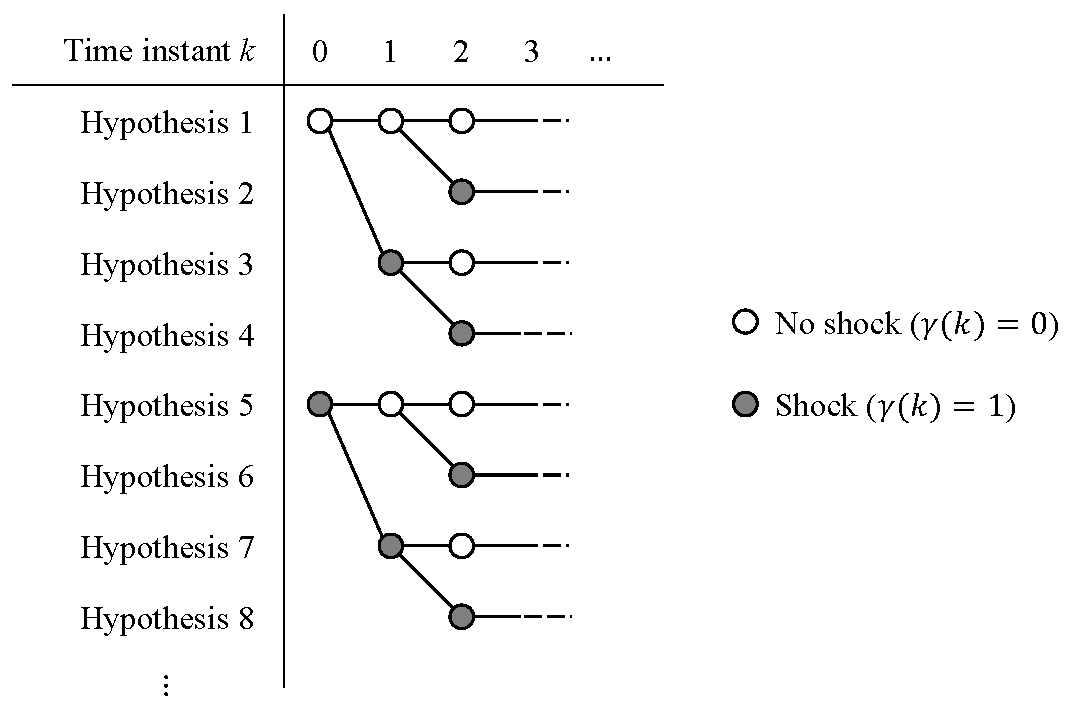
\includegraphics[height=7.5cm]{images/mm_obs_seq_br.pdf}
	\caption{Sequence branching}
	\label{fig:mm-obs-br}
\end{figure}

\subsubsection{Generalised pseudo-Bayes algorithm} \label{sec:GPB}

One of the simplest sub-optimal multiple-model methods is the \textit{generalised pseudo-Bayesian algorithm} \citep{buxbaum_recursive_1969, jaffer_estimation_1971, tugnait_detection_1982}. Although not used directly in this work, the method is described here because it is a starting point for understanding hypotheses branching and merging, which are techniques used in the sequence fusion algorithm described by \cite{robertson_detection_1995}.

There are two basic versions of the algorithm, the \acrlong{GPB1} (\acrshort{GPB1}), and the \acrlong{GPB2} (\acrshort{GPB2}). Figure \ref{fig:mm-obs-gpb1} shows a simplified diagram of the \gls{GPB1} process in the case of a system with two modes ($n_j=2$). A single estimate of the system states and error covariance at time $k$ is branched into $n_j$ hypotheses representing the possible modes of the system at that time. In this context, \textit{branching} simply means duplicating or cloning the hypothesis state estimates and error covariance into $n_j$ copies. These are then used to initialise $n_j$ Kalman filters. Each Kalman filter then makes a prediction of the states in the next time instant using the system model associated with one of the possible modes. In the next time instant, the $n_j$ predictions are corrected using the measurements, and the updated estimates are merged into a single set of estimates using the multiple-model observer merging procedure defined by (\ref{eq:xkyk_hat_MKF}, \ref{eq:Pk_MKF}). These branching and merging steps are then repeated at each subsequent time step.
\begin{figure}[ht]
	\centering
	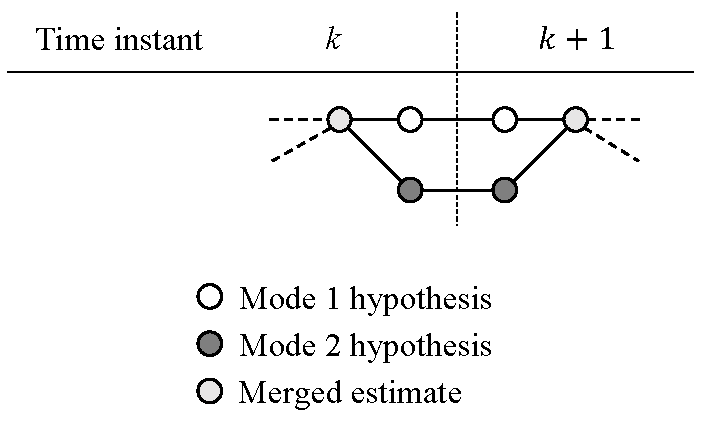
\includegraphics[height=5cm]{images/mm_obs_seq_gpb1.pdf}
	\caption{Simplified diagram of the \gls{GPB1} algorithm ($n_j=2$)}
	\label{fig:mm-obs-gpb1}
\end{figure}

Whereas the \gls{GPB1} estimator considers $n_j$ possible mode transitions from time $k-1$ to time $k$, the \gls{GPB2} estimator considers $n_j^2$ possible transition sequences from time $k-2$ to time $k$. Figure \ref{fig:mm-obs-gpb2} shows a simplified diagram of the \gls{GPB2} algorithm in the case of two system modes ($n_j=2$). At time $k$ it maintains $n_j$ merged estimates and associated variables, $\left\{ \hat{\mathbf{x}}_m(k \mid k), \mathbf{P}_m(k \mid k), \hat{\mathbf{y}}_m(k \mid k), \Pr(\Gamma_m(k) \mid \mathbf{Y}_M(k)) \right\}$, for $m=1,2,...,n_j$. Each of these is then branched into $n_j$ estimates, creating a total of $n_h=n_j^2$ hypotheses, represented by $n_h$ Kalman filters labelled $f=1,2,...n_h$. At time $k+1$, the Kalman filter predictions are corrected to produce $n_h$ estimates. Then, two merging operations are carried out on these estimates. The first merges the $n_h$ estimates into $n_m=n_j$ estimates for use in the next step. The second merges the $n_m$ merged estimates again, into one final estimate which is the output of the observer and is not used in subsequent steps.
\begin{figure}[ht]
	\centering
	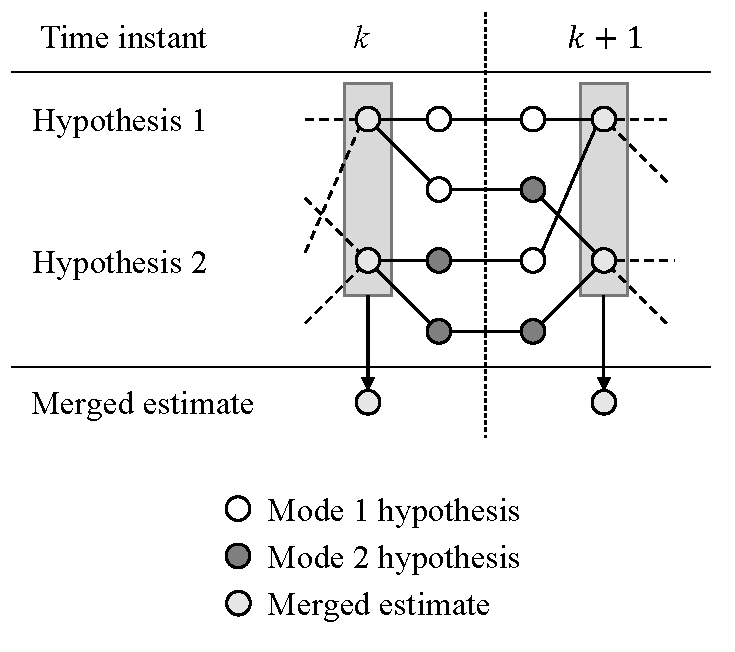
\includegraphics[height=6.5cm]{images/gpb2_diagram.pdf}
	\caption{Simplified diagram of the \gls{GPB2} algorithm ($n_j=2$)}
	\label{fig:mm-obs-gpb2}
\end{figure}

The $n_m$ merged estimates and covariances at time $k$ are produced by calculating weighted sums of the estimates and covariances of the branched hypotheses,
\nomenclature{$n_m$}{number of merged hypotheses maintained by a multiple-model observer}%
\nomenclature{$\mathbf{\hat{x}}_m(k \mid k)$}{merged estimates of the system states at time $k$ for merged hypothesis $m$}%
\nomenclature{$\mathbf{\hat{y}}_m(k \mid k)$}{merged estimates of the system outputs at time $k$ for merged hypothesis $m$}%
\nomenclature{$\mathbf{P}_m(k \mid k)$}{merged state estimation error covariance at time $k$ for merged hypothesis $m$}%
\nomenclature{$\Gamma_m(k)$}{merged shock hypothesis $m$ at time $k$}%
\begin{equation} \label{eq:xmkymk_hat_MKF}
	\begin{aligned}
		\mathbf{\hat{x}}_m(k \mid k) = \frac{1}{Z_m(k)} \sum_{f \in \mathcal{H}_{\text{merge},m}} \mathbf{\hat{x}}_f(k \mid k) \Pr(\Gamma_f(k) \mid \mathbf{Y}_M(k)), \\
		\mathbf{\hat{y}}_m(k \mid k) = \frac{1}{Z_m(k)} \sum_{f \in \mathcal{H}_{\text{merge},m}} \mathbf{\hat{y}}_f(k \mid k) \Pr(\Gamma_f(k) \mid \mathbf{Y}_M(k)),\\
		\mathbf{P}_m(k \mid k) = \frac{1}{Z_m(k)} \sum_{f \in \mathcal{H}_{\text{merge},m}} \Pr(\Gamma_f(k) \mid \mathbf{Y}_M(k)) \left( \mathbf{P}_f(k \mid k) + \delta_\mathbf{\hat{x}}(k) \delta_\mathbf{\hat{x}}^\intercal(k) \right), \\
		\delta_\mathbf{\hat{x}}(k) = \mathbf{\hat{x}}_m(k \mid k) - \mathbf{\hat{x}}_f(k \mid k), \\
		\Pr(\Gamma_m(k) \mid \mathbf{Y}_M(k)) = \sum_{f \in \mathcal{H}_{\text{merge},m}} \Pr(\Gamma_f(k) \mid \mathbf{Y}_M(k)).
	\end{aligned}
\end{equation}
\nomenclature{$\mathcal{H}_{\text{merge}}$}{hypothesis index used in merging operations}%
where $\mathcal{H}_{\text{merge}}$ is a set of $n_m$ indices that determine which hypotheses are merged to produce each merged estimate, and $Z_m(k)$ is a scalar normalization variable given by
\nomenclature{$Z_m(k)$}{normalization variable at time $k$ used in merged probability calculations}%
\begin{equation} \label{eq:Zmk}
	Z_m(k) = \sum_{f \in \mathcal{H}_{\text{merge},m}} \Pr(\Gamma_f(k) \mid \mathbf{Y}_M(k)).
\end{equation}

In the case of \gls{GPB2}, $\mathcal{H}_{\text{merge}}$ is defined
\begin{equation} \label{eq:Hmerge_GPB2}
	\mathcal{H}_{\text{merge}} = \begin{Bmatrix} \mathcal{H}_{\text{merge},1} \\ \mathcal{H}_{\text{merge},2} \end{Bmatrix} = \begin{Bmatrix}
		\begin{bmatrix}	1 \\ 3 \end{bmatrix} \\
		\begin{bmatrix}	2 \\ 4 \end{bmatrix}
	\end{Bmatrix}.
\end{equation}
This means that merged estimate $\mathbf{\hat{x}}_1(k \mid k)$ is calculated by merging the estimates associated with branched hypotheses 1 and 3, and merged estimate $\mathbf{\hat{x}}_2(k \mid k)$ is calculated by merging the estimates of branched hypotheses 2 and 4.

An associated index, $\mathcal{H}_{\text{branch}}$, governs the branching operation, which for \gls{GPB2} is
\nomenclature{$\mathcal{H}_{\text{branch}}$}{hypothesis index used in branching operations}%
\begin{equation} \label{eq:Hbranch_GPB2}
	\mathcal{H}_{\text{branch}} = \begin{bmatrix} 1 \\ 1 \\ 2 \\ 2 \end{bmatrix}.
\end{equation}
This indicates that branched estimates 1 and 2 are clones of merged estimate $\mathbf{\hat{x}}_1(k \mid k)$ and branched estimates 3 and 4 are clones of merged estimate $\mathbf{\hat{x}}_2(k \mid k)$. These definitions match the branching and merging operations depicted in Figure \ref{fig:mm-obs-gpb2}.

% TODO: We don't need this if we define the r(k) and r_m(k) transitions.
The system modes, which determine the system model parameters as well as the mode transition probabilities, evolve according to the branching and merging indices. Starting with the modes associated with the merged hypotheses at time $k$, which in the case of GPB2 are
\nomenclature{$\mathbf{r}_m(k)$}{indicators of the system modes of the merged hypotheses at time $k$ used in branching and merging operations}%
\begin{equation} \label{eq:rmk_GPB2}
		\mathbf{r}_m(k) = \begin{bmatrix} 1 \\ 2 \end{bmatrix},
\end{equation}
the branched modes after branching at time $k$ and before merging at time $k+1$ are
\nomenclature{$\mathbf{r}_{b,1}(k)$}{indicators of the system modes of the branched hypotheses at time $k$ before merging}%
\nomenclature{$\mathbf{r}_{b,2}(k)$}{indicators of the system modes of the branched hypotheses at time $k$ after branching}%
\begin{equation} \label{eq:rbk_GPB2}
	\begin{aligned}
		\mathbf{r}_{b,2}(k) &= \begin{bmatrix} 1 \\ 1 \\ 2 \\ 2 \end{bmatrix},
		\mathbf{r}_{b,1}(k+1) &= \begin{bmatrix} 1 \\ 2 \\ 1 \\ 2 \end{bmatrix}.
	\end{aligned}
\end{equation}
Note that $\mathbf{r}_{b,2}(k)$ is derived by branching $\mathbf{r}_m(k)$ using $\mathcal{H}_{\text{branch}}$ and that when $\mathbf{r}_{b,1}(k+1)$ is merged using $\mathcal{H}_{\text{merge}}$ in the next time step, it leads to 
\begin{equation} \label{eq:rmkp1rmk_GPB2}
	\mathbf{r}_m(k+1) = \begin{bmatrix} 1 \\ 2 \end{bmatrix} = \mathbf{r}_m(k).
\end{equation}
Due to this condition, the algorithm is consistent when executed consecutively every time step.

The advantages of the \gls{GPB1} and \gls{GPB2} estimators are their simplicity, the fact that they can be applied to any switching system, and that the number of hypotheses ($n_j$ or $n_j^2$) is finite and constant, which limits computational requirements. The disadvantages include the fact that they model every possible transition over one or two time steps and merge these into a reduced set of estimates before the next iteration. 

While the branching, modes, and merging steps of the \gls{GPB1} and \gls{GPB2} algorithms are the same each time step, they may be time-varying in the case of the sub-optimal multiple-model algorithms considered in this work. The notation above is easily extended to more complex algorithms with arbitrary branching and merging steps by allowing $\mathcal{H}_{\text{branch}}$, $\mathcal{H}_{\text{merge}}$, $\mathbf{r}_{b,1}(k)$, and $\mathbf{r}_{b,2}(k)$ to be time-varying and by allowing an arbitrarily large number of branched and merged hypotheses, $n_h$ and $n_m$, to exist at each time instant.

\subsubsection{Sequence fusion} \label{sec:fusion}

\cite{robertson_detection_1995} proposed a sub-optimal approach that combines three approximation techniques specifically intended for \gls{RODD} state estimation. The first is referred to as \textit{sequence fusion}. This is based on the assumption that only recent differences in the hypothesis sequences are important for state estimation. Therefore, sequences that are identical over the previous $N_f$ sample times may be merged, where $N_f$ is known as the \textit{fusion horizon}.
\nomenclature{$N_f$}{sequence fusion parameter: length of fusion horizon in number of sampling intervals}%
%The same techniques used in the generalized pseudo-Bayes algorithm are used to perform the sequence branching and merging at each time step. The differences are that more than $n_j^2$ hypotheses are maintained and these are based on longer, pre-specified sequences of possible shocks.

Rather than allowing the number and length of the shock indicator hypothesis sequences, $\Gamma_f(k)$, to grow indefinitely, a fixed number of sequences of length $N_f$ sample periods are defined, each consisting of only the current and the previous $N_f-1$ values of \hl{$\gamma(k)$}
\nomenclature{$\Gamma_m(k-N_f+1,k)$}{merged shock hypotheses $m$ at time $k$ for the fusion horizon $N_f$}%
\begin{equation} \label{eq:Gamma_kmf_k}
	\Gamma_m(k-N_f+1,k) = \{\gamma_m(k-N_f+1), ...,  \gamma_m(k-1), \gamma_m(k)\}, m=1,2,..., n_m.
\end{equation}
These fixed-length sequences are used to merge similar hypotheses so that the total number, $n_m$, remains the same from one time instant to the next.

Secondly, they assume that the exact timing of random shocks is not important and define \textit{detection intervals} of more than one sample period during which it is assumed that only one shock may occur. This is based on the observation that when the correction gain of a Kalman filter increases due to the assumption of a shock occurrence ($\gamma_m(k)=1$), it tends to remain large for several sample periods. The probability of at least one random shock during a detection interval of length $d$ samples is therefore higher than the probability, $\varepsilon$, of a single shock in one sample period, and is given by
\nomenclature{$d$}{sequence fusion parameter: shock spacing or length of detection interval, in number of sampling intervals}
\nomenclature{$\varepsilon_d$}{sequence fusion parameter: probability of at least one shock within the detection interval}%
\begin{equation}  \label{eq:p_gamma_d}
	\varepsilon_d = 1 - (1 - \varepsilon)^{d}.
\end{equation}

The occurrence of one or more shocks within a detection interval is then represented by a single shock at the start of the detection interval and the probabilities of a shock at any other time are set to zero,
\begin{equation} \label{eq:Pr_gamma_nd}
	\begin{aligned}
		\Pr\left(\gamma_{f}(k)=0\right) = \begin{cases*}
			1 - \varepsilon_d & \text { for } $k = d, 2d, 3d, \ldots$ \\
			1 & \text { for } $k \ne d, 2d, 3d, \ldots$
		\end{cases*} \\
		\Pr\left(\gamma_{f}(k)=1\right) = \begin{cases*}
			\varepsilon_d & \text { for } $k = d, 2d, 3d, \ldots$ \\
			0 & \text { for } $k \ne d, 2d, 3d, \ldots$
		\end{cases*} \\
	\end{aligned}
\end{equation}

Thirdly, they rely on the fact that the random shocks occur infrequently and therefore the probability of more than $n_\text{max}$ shocks during the fusion horizon is low, where $n_\text{max}$ may be 1 or some other low number. This further reduces the number of possible hypotheses that must be modelled.
\nomenclature{$n_\text{max}$}{sequence fusion parameter: maximum number of shock occurrences within the fusion horizon}%

To illustrate the resulting shock hypothesis sequences, consider an example. Suppose there is one \gls{RODD} to estimate. A sequence fusion algorithm is used with a fusion horizon of $N_f=9$, a detection interval of $d=3$, and a maximum number of shocks over the fusion horizon of $n_\text{max}=1$. Figure \ref{fig:mm-obs-seq-SFex1} shows the four shock hypotheses that would be required in this case. Note that hypothesis 1 assumes no shocks at any time. Hypothesis 2 assumes shocks occur at times $k=0,9,18,...$. Hypothesis 3 assumes shocks occur at times $k=3,12,21,...$, and so on. After $N_f=9$ sample periods, the sequences repeat indefinitely.

\begin{figure}[ht]
	\centering
	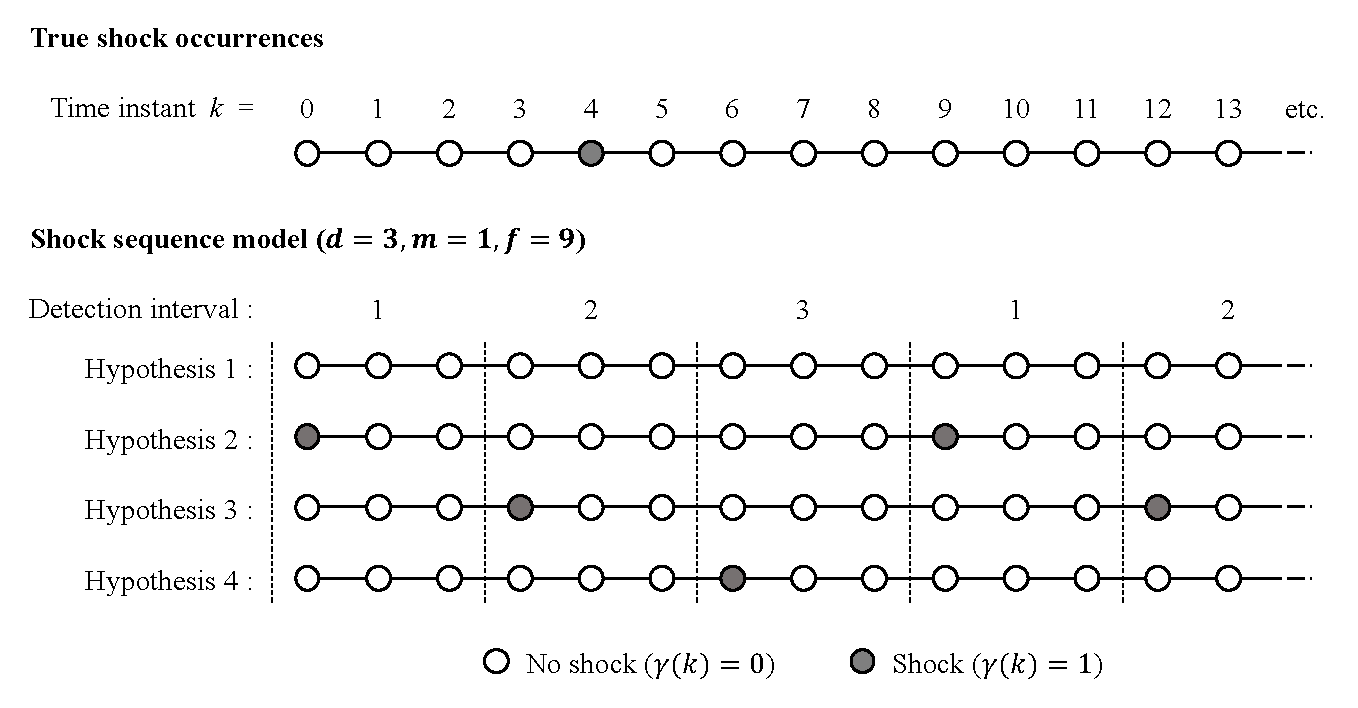
\includegraphics[width=13.5cm]{images/mm_obs_seq_rob1.pdf}
	\caption{Sequence fusion example 1 ($N_f=9$, $n_\text{max}=1$, $d=3$)}
	\label{fig:mm-obs-seq-SFex1}
\end{figure}

Suppose that a shock actually occurred in the system at time $k=4$. In this case, the algorithm should predict that hypothesis 3 is the most likely because this assumes a shock occurred at $k=3$, which is the closest to the actual time.

Figure \ref{fig:mm-obs-seq-SFex2} illustrates a second example with $N_f=10$, $n_\text{max}=2$, and $d=5$. This also has four hypotheses. However, note that hypothesis 4 accounts for the possibility of two shocks within the fusion horizon. As in the previous example, if a true shock occurred at time $k=4$, the most likely hypothesis should be hypothesis 3 because it assumes a shock occurred at $k=5$, which is close to the actual time.
\begin{figure}[ht]
	\centering
	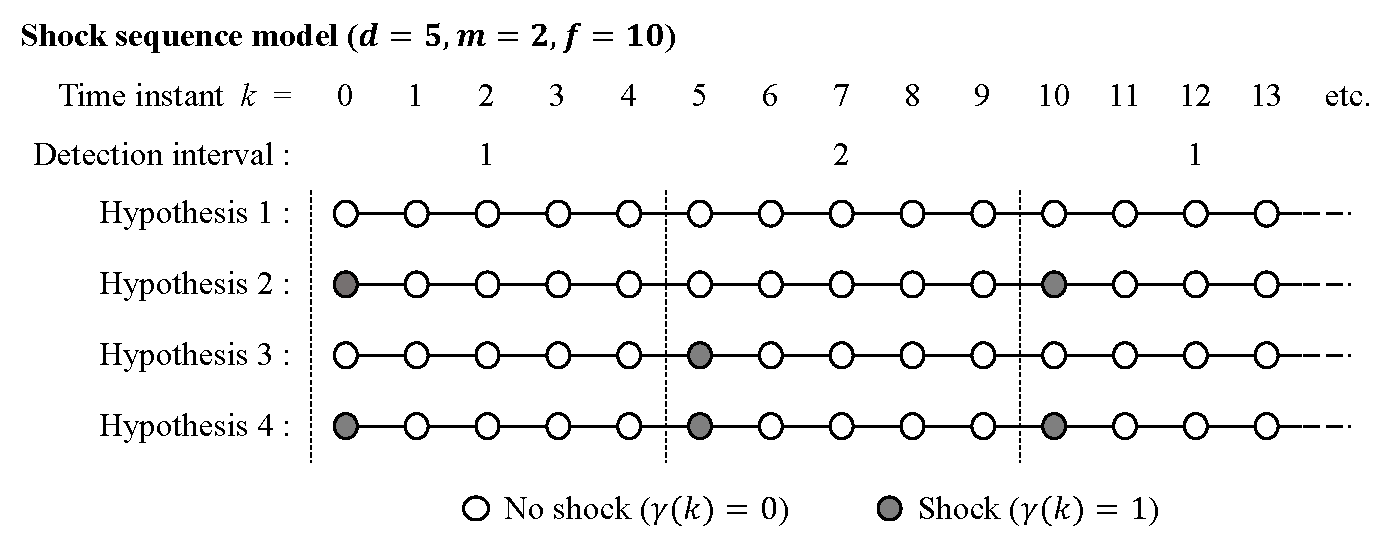
\includegraphics[width=13.5cm]{images/mm_obs_seq_rob2.pdf}
	\caption{Sequence fusion example 2 ($N_f=10$, $n_\text{max}=2$, $d=5$)}
	\label{fig:mm-obs-seq-SFex2}
\end{figure}

As mentioned, the shock hypothesis sequences over the fusion horizon, $\Gamma_m(k-N_f+1,k)$, determine the branching and merging operations that occur at each time step. The logic is as follows: (i) at time $k$, branch each hypothesis sequence into the possible mode transitions that occur between time $k$ and $k+1$, (ii) advance the branched sequences into the next time step, according to the possible mode transitions, (iii) compare the branched sequences and merge those that are identical over the new fusion horizon from time $k-N_f+2$ to $k+1$.

Consider again the sequences from the previous example in Figure \ref{fig:mm-obs-seq-SFex2}. By applying the logic described above, the branching and merging operations depicted in Figure \ref{fig:mm-obs-seq-sf95} may be deduced. For example, consider what happens at time $k=9$. At this time, the fusion horizon spans from time 0 to 9. The four sequences are branched into eight and advanced to the next time instant according to the possible modes at that time (no shock, shock). Then, at time $k=10$ the 8 branched hypotheses are merged back to 4 by combining sequences that are identical over the new fusion horizon, which spans from $k=1$ to 10. Applying this logic each time step, branching and merging are only required once every 5 time steps when shocks are assumed to be possible.
\begin{figure}[ht]
	\centering
	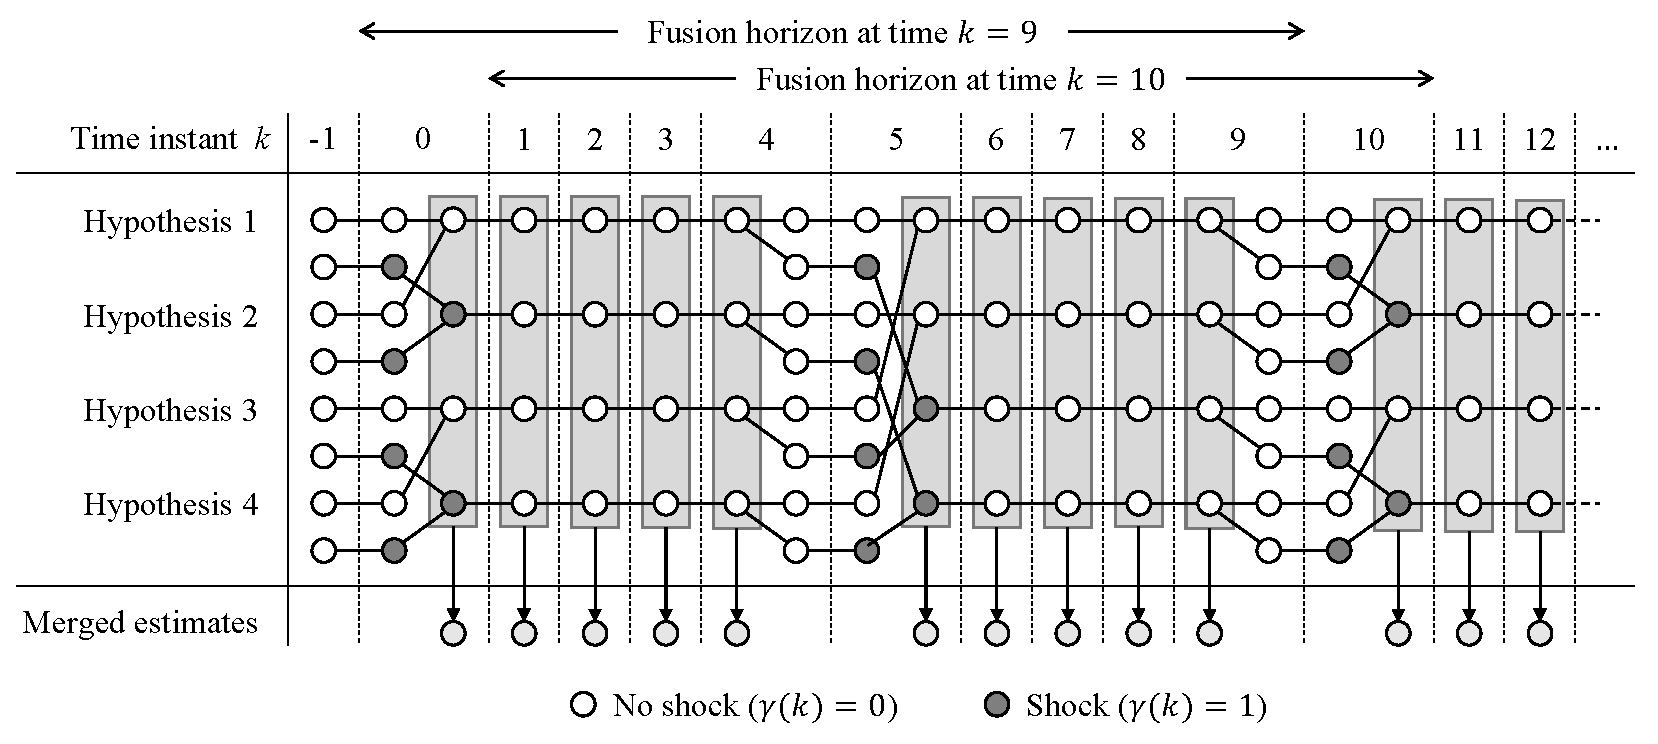
\includegraphics[width=15.5cm]{images/mm_obs_seq_sf95.pdf}
	\caption{Sequence branching and merging example ($N_f=10$, $n_\text{max}=2$, $d=5$)}
	\label{fig:mm-obs-seq-sf95}
\end{figure}

Rather than constant branching and merging indices, as in GPB2 (\ref{eq:Hbranch_GPB2}, \ref{eq:Hmerge_GPB2}), sequences of branching and merging indices are needed. In this example, they are
\begin{equation} \label{eq:Hbranch_SFex2}
	\mathcal{H}_{\text{branch}} = \begin{Bmatrix}
		\begin{bmatrix} 1 \\ 2 \\ 3 \\ 4 \end{bmatrix} &
		\begin{bmatrix} 1 \\ 2 \\ 3 \\ 4 \end{bmatrix} &
		\begin{bmatrix} 1 \\ 2 \\ 3 \\ 4 \end{bmatrix} &
		\begin{bmatrix} 1 \\ 2 \\ 3 \\ 4 \end{bmatrix} &
		\begin{bmatrix} 1 \\ 1 \\ 2 \\ 2 \\ 3 \\ 3 \\ 4 \\ 4 \end{bmatrix} &
		\begin{bmatrix} 1 \\ 2 \\ 3 \\ 4 \end{bmatrix} &
		\begin{bmatrix} 1 \\ 2 \\ 3 \\ 4 \end{bmatrix} &
		\begin{bmatrix} 1 \\ 2 \\ 3 \\ 4 \end{bmatrix} &
		\begin{bmatrix} 1 \\ 2 \\ 3 \\ 4 \end{bmatrix} &
		\begin{bmatrix} 1 \\ 1 \\ 2 \\ 2 \\ 3 \\ 3 \\ 4 \\ 4 \end{bmatrix}
	\end{Bmatrix},
\end{equation}
and
\begin{equation} \label{eq:Hmerge_SFex2}
	\mathcal{H}_{\text{merge}} = \begin{Bmatrix}
		\begin{bmatrix}	1 \\ 3 \end{bmatrix} & 1 & 1 & 1 & 1 & \begin{bmatrix}	1 \\ 5 \end{bmatrix} & 1 & 1 & 1 & 1 \\
		\begin{bmatrix}	2 \\ 4 \end{bmatrix} & 2 & 2 & 2 & 2 & \begin{bmatrix}	3 \\ 7 \end{bmatrix} & 2 & 2 & 2 & 2 \\
		\begin{bmatrix}	5 \\ 7 \end{bmatrix} & 3 & 3 & 3 & 3 & \begin{bmatrix}	2 \\ 6 \end{bmatrix} & 3 & 3 & 3 & 3 \\
		\begin{bmatrix}	6 \\ 8 \end{bmatrix} & 4 & 4 & 4 & 4 & \begin{bmatrix}	4 \\ 8 \end{bmatrix} & 4 & 4 & 4 & 4 \\
	\end{Bmatrix}.
\end{equation}

% Remove these: they don't add anything since these can be derived from the sequence
% and the branching/merging indices. Also, this convention for \Gamma_b and \Gamma_m
% was not defined. \Gamma_f was defined as single sequence and arguably would be
% better restricted to the merged sequences, than the branched ones.
%Likewise, the merged and branched shock (mode) indicator sequences are
%\begin{multline} \label{eq:Gamma_km09}
%	\glsadd{Gammafkmnk}\Gamma_m(0,9) = \left\{
%		\mathbf{\gamma}_m(0), \mathbf{\gamma}_m(1), \cdots, \mathbf{\gamma}_m(9)
%	\right\} = \\ 
%	\left\{
%		\begin{bmatrix} 0 \\ 1 \\ 0 \\ 1 \end{bmatrix},
%		\begin{bmatrix} 0 \\ 0 \\ 0 \\ 0 \end{bmatrix},
%		\begin{bmatrix} 0 \\ 0 \\ 0 \\ 0 \end{bmatrix},
%		\begin{bmatrix} 0 \\ 0 \\ 0 \\ 0 \end{bmatrix},
%		\begin{bmatrix} 0 \\ 0 \\ 0 \\ 0 \end{bmatrix},
%		\begin{bmatrix} 0 \\ 0 \\ 1 \\ 1 \end{bmatrix},
%		\begin{bmatrix} 0 \\ 0 \\ 0 \\ 0 \end{bmatrix},
%		\begin{bmatrix} 0 \\ 0 \\ 0 \\ 0 \end{bmatrix},
%		\begin{bmatrix} 0 \\ 0 \\ 0 \\ 0 \end{bmatrix},
%		\begin{bmatrix} 0 \\ 0 \\ 0 \\ 0 \end{bmatrix}
%	\right\}.
%\end{multline}
%\begin{multline} \label{eq:Gamma_kb09}
%		\Gamma_b(0,9 \mid 9) = \left\{\mathbf{\gamma}_b(0 \mid 0), \mathbf{\gamma}_b(1 \mid 1), \cdots, \mathbf{\gamma}_b(9 \mid 9) \right\} = \\
%		\left\{
%			\begin{bmatrix} 0 \\ 0 \\ 0 \\ 0 \end{bmatrix},
%			\begin{bmatrix} 0 \\ 0 \\ 0 \\ 0 \end{bmatrix},
%			\begin{bmatrix} 0 \\ 0 \\ 0 \\ 0 \end{bmatrix},
%			\begin{bmatrix} 0 \\ 0 \\ 0 \\ 0 \end{bmatrix},
%			\begin{bmatrix} 0 \\ 0 \\ 0 \\ 0 \\ 1 \\ 1 \\ 1 \\ 1 \end{bmatrix},
%			\begin{bmatrix} 0 \\ 0 \\ 0 \\ 0 \end{bmatrix},
%			\begin{bmatrix} 0 \\ 0 \\ 0 \\ 0 \end{bmatrix},
%			\begin{bmatrix} 0 \\ 0 \\ 0 \\ 0 \end{bmatrix},
%			\begin{bmatrix} 0 \\ 0 \\ 0 \\ 0 \end{bmatrix}
%			\begin{bmatrix} 0 \\ 0 \\ 1 \\ 1 \\ 0 \\ 0 \\ 1 \\ 1 \end{bmatrix},
%		\right\},
%\end{multline}
%\begin{multline} \label{eq:Gamma_kb110}
%		\Gamma_b(1,10 \mid 9) = \left\{ \mathbf{\gamma}_b(1 \mid 0), \mathbf{\gamma}_b(2 \mid 1), \cdots, \mathbf{\gamma}_b(10 \mid 9) \right\} = \\
%		\left\{
%			\begin{bmatrix} 0 \\ 1 \\ 0 \\ 1 \\ 0 \\ 1 \\ 0 \\ 1 \end{bmatrix},
%			\begin{bmatrix} 0 \\ 0 \\ 0 \\ 0 \end{bmatrix},
%			\begin{bmatrix} 0 \\ 0 \\ 0 \\ 0 \end{bmatrix},
%			\begin{bmatrix} 0 \\ 0 \\ 0 \\ 0 \end{bmatrix},
%			\begin{bmatrix} 0 \\ 0 \\ 0 \\ 0 \end{bmatrix},
%			\begin{bmatrix} 0 \\ 1 \\ 0 \\ 1 \\ 0 \\ 1 \\ 0 \\ 1 \end{bmatrix},
%			\begin{bmatrix} 0 \\ 0 \\ 0 \\ 0 \end{bmatrix},
%			\begin{bmatrix} 0 \\ 0 \\ 0 \\ 0 \end{bmatrix},
%			\begin{bmatrix} 0 \\ 0 \\ 0 \\ 0 \end{bmatrix},
%			\begin{bmatrix} 0 \\ 0 \\ 0 \\ 0 \end{bmatrix}
%		\right\}.
%\end{multline}
Although the number of branched hypotheses is time-varying, after $N_f$ time steps the sequences repeat such that
\nomenclature{$\mathbf{\gamma}_m(k)$}{vector of random shock indicators, $\gamma_f(k)$ for $f=1,2,...,m$, at time $k$}%
\begin{equation} \label{eq:rmkrmkmNf_SFex2}
	\mathbf{\gamma}_m(k) = \mathbf{\gamma}_m(k-N_f).
\end{equation}

As in the \gls{GPB2} algorithm, the overall estimates of the system states and outputs, $\hat{\mathbf{x}}(k \mid k)$ and $\hat{\mathbf{y}}(k \mid k)$, are calculated by merging the partially-merged estimates into one overall estimate. This is achieved by substituting $\mathbf{\hat{x}}_m(k \mid k)$ and $\mathbf{\hat{y}}_m(k \mid k)$ for $\mathbf{\hat{x}}_f(k \mid k)$ and $\mathbf{\hat{y}}_f(k \mid k)$ in \eqref{eq:xkyk_hat_MKF}.

\cite{robertson_detection_1995} described a systematic procedure to choose the parameters $N_f$, $n_\text{max}$, and $d$ and give the formula for the total probability of the modelled hypotheses as
\begin{equation} \label{eq:p_gamma}
	\beta=\operatorname{Pr}\left(\sum_{i=1}^{n} \gamma(i d) \leq n_\text{max} \right) = \sum_{j=0}^{n_\text{max}} \binom{n}{j} \varepsilon_d^{n-j}(1-\varepsilon_d)^{j},
\end{equation}
\nomenclature{$\beta$}{sequence fusion paramter: total probability of the modelled hypotheses, or in the case of the \acrshort{BRW}, a parameter of the additive bias function $a(\cdot)$}%
where $\binom{n}{j}$ represents the number of possible combinations of $j$ shocks in $n$ detection intervals. They recommended that the total probability should be at least 0.99 to ensure that only low-probability hypotheses are ignored.

In a later journal paper, \cite{robertson_method_1998} described a variation to the sequence fusion algorithm described above.  Rather than assuming that the shock occurs in the first sample period of each detection interval, as shown in Figures \ref{fig:mm-obs-seq-SFex1} and \ref{fig:mm-obs-seq-SFex2}, they proposed to represent the possibility of a shock as a sequence of $d$ smaller shocks such that the total variance over the detection interval is the same as that of one shock. They claimed this improved the performance of the algorithm in their simulations.

To implement this modification, define a new variable, $\delta(n)$, to represent whether or not at least one shock occurred during the $n$\textsuperscript{th} detection interval:
\nomenclature{$\delta(n)$}{sequence fusion variable: indicator of whether one or more shocks occurred in detection interval $n$}
\begin{equation} \label{eq:deltak}
	\delta(n) = \begin{cases*}
		0 & \text{if} $\sum_{k=(n-1) d}^{n d - 1}{\gamma(k)} = 0$, \\
		1 & \text{if} $\sum_{k=(n-1) d}^{n d - 1}{\gamma(k)} \ge 1$.
	\end{cases*}
\end{equation}

Then, replace the random shock variable used at each sample time, $w_p(k)$ \eqref{eq:wpk2}, with:
\begin{equation} \label{eq:wpdk}
	w_{p,d}(k) \sim 
	\begin{cases*}
		\mathcal{N}\left(0, \sigma_{w_p}^2\right) & \text{when} $\delta(n) = 0$, \\
		\mathcal{N}\left(0, \frac{b^2\sigma_{w_p}^2}{d}\right) & \text{when} $\delta(n) = 1$.
	\end{cases*}
\end{equation}

Note that the variance of a single shock, $b^2\sigma_{w_p}^2$, has ben divided by the detection interval length $d$. In this version of the algorithm, the branching and merging operations are only carried out at the end of each detection interval. In the steps within the detection interval, the Kalman filters are updated using the measurements, but no branching or merging occurs.

Figure \ref{fig:mm-obs-seq-sf98} shows the shock hypothesis sequences and the merging and branching steps of the 1998 version of the sequence fusion algorithm with the same parameters as in the previous example.
\begin{figure}[ht]
	\centering
	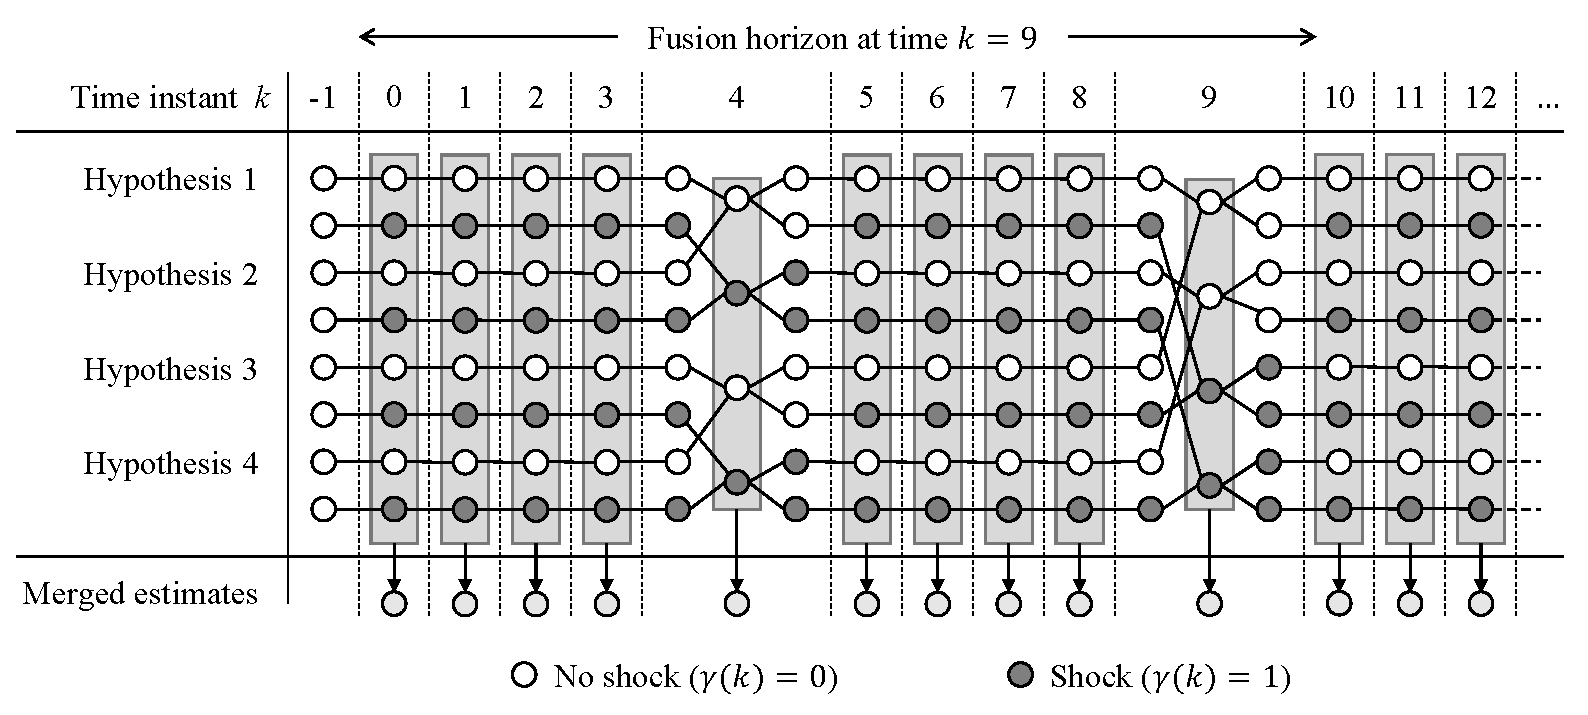
\includegraphics[width=15cm]{images/mm_obs_seq_sf98.pdf}
	\caption{Sequence branching and merging example – 1998 version ($N_d=5$, $n_\text{max}=2$, $N_f=10$)}
	\label{fig:mm-obs-seq-sf98}
\end{figure}
Note the two main differences when compared to Figure \ref{fig:mm-obs-seq-sf95}. Firstly, the system mode indicators are the same throughout the detection interval, whereas in the 1995 version the shocks were assumed to occur only at the first sample time of each detection interval. Secondly, after branching, the $n_h$ hypotheses are maintained for the duration of the detection interval before being merged and branched at the last sample time of the detection interval. The idea of these modifications is to allow $N_d$ Kalman filter updates to occur with the adjusted shock probability and variance (\ref{eq:p_gamma_d}, \ref{eq:wpdk}) before evaluating and merging the estimates. This was expected to produce better estimates of the hypothesis probabilities in situations where it takes more than one time step to detect changes in the system.

\subsubsection{Sequence pruning} \label{sec:pruning}

\textit{Sequence pruning} is the selective deletion of shock hypotheses that have a low likelihood given the current measurements. \cite{eriksson_classification_1996} used the \textit{adaptive forgetting through multiple models} (\acrshort{AFMM}) algorithm by \cite{andersson_adaptive_1985} for \gls{RODD} estimation. The \gls{AFMM} uses sequence pruning to limit the number of hypotheses and filters. The current hypotheses at each time instant are ranked according to their conditional probabilities \eqref{eq:Pr_Gammak_given_Yk}. The hypothesis with the lowest probability is then pruned with the caveat explained below. The most probable hypothesis is allowed to branch but all other hypotheses are advanced assuming no shock occurs in the next time period (i.e. all but one of their branches are pruned). This makes sense in the case of \gls{RODD} disturbances because the probability of a shock is low. Thus, the total number of hypotheses and filters is capped at a fixed number, $n_h$.

The caveat mentioned above, is that no hypothesis may be eliminated less than $N_\text{min}$ time steps after being created. This is to prevent good hypotheses from being eliminated before the conditional probabilities have been properly estimated, which can take more than one sample period. For this reason, $n_h$ must be at least sufficient to accommodate the \textit{minimum life}, $N_\text{min}$, of all new hypotheses. Note that in the case of systems with more than one \gls{RODD} disturbance, the number of branches of the most likely sequence is more than two, \hl{and the same number} of sequences will be pruned at each sample time.
\nomenclature{$N_\text{min}$}{sequence pruning parameter: minimum life of a branched hypothesis in number of sampling intervals}%

To illustrate the sequence pruning procedure, consider the diagram in Figure \ref{fig:mm-obs-seq-SP}. This shows one possible evolution of the hypothesis sequences in response to an actual shock sequence consisting of one shock at time $k=4$.  The most likely hypotheses at each time instant, identified by the circles with thicker outlines, branch into two at the next time instant. After the limit of five hypotheses is reached, one hypothesis is pruned at each sample time and replaced by a new branched hypothesis at the next. Note that at time $k=6$, hypothesis 2 becomes the most likely based on the available measurements at that time. Also note that no new branches are terminated in less than two sample times.
\begin{figure}[ht]
	\centering
	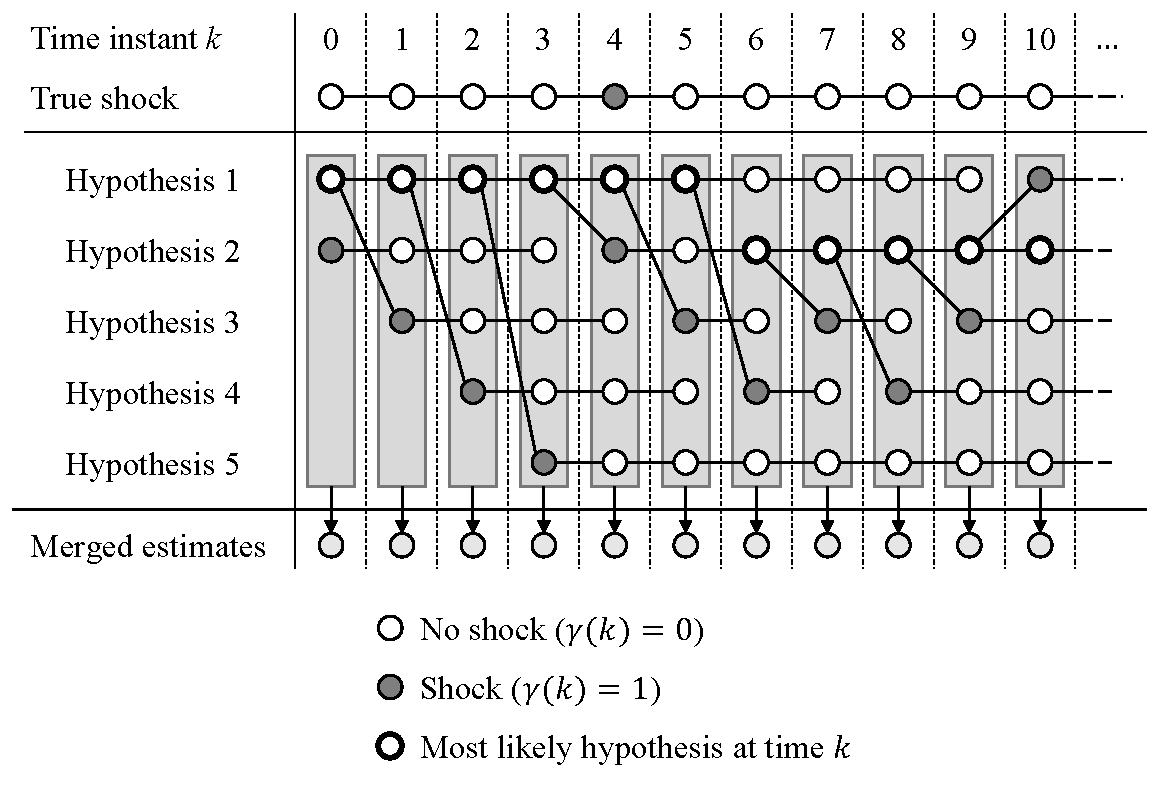
\includegraphics[width=10.7cm]{images/mm_obs_seq_SP.pdf}
	\caption{Sequence pruning example ($n_h=5$, $N_\text{min}=2$)}
	\label{fig:mm-obs-seq-SP}
\end{figure}

The \gls{AFMM} algorithm includes a complementary procedure for online estimation of the measurement noise covariance, $\mathrm{R}(k)$. This component was not implemented in this work since it is assumed that the variance of the measurement noise is time-invariant.

\subsubsection{Implementation details} \label{sec:implementation}

The diagram in Figure \ref{fig:mkf-infoflow} depicts the general computation steps and information flows of the sub-optimal multiple-model observers, as implemented in this work. The solid black rectangles represent computation steps and the \hl{coloured lines} represent the main variables. Steps 1 and 2 are the prediction steps of the Kalman filters (\ref{eq:xfkp1_hat}, \ref{eq:yfk_pred}), step 3 is the calculation of the prior probabilities of the hypotheses \eqref{eq:Pr_Gammak_given_Ykm1}, step 4 is the hypotheses evaluation step (\ref{eq:Pr_Gammak_given_Yk}, \ref{eq:qfk}), and step 5 is the Kalman filter update step (\ref{eq:xfkyfk_hat}, \ref{eq:Pkf-stab}). Step 6 is a place-holder for the sub-optimal procedures which depend on the specific algorithm but in this work include some combination of sequence branching, pruning, and merging. During this step, the final estimates of the states and outputs are also calculated.

\begin{figure}[ht]
	\centering
	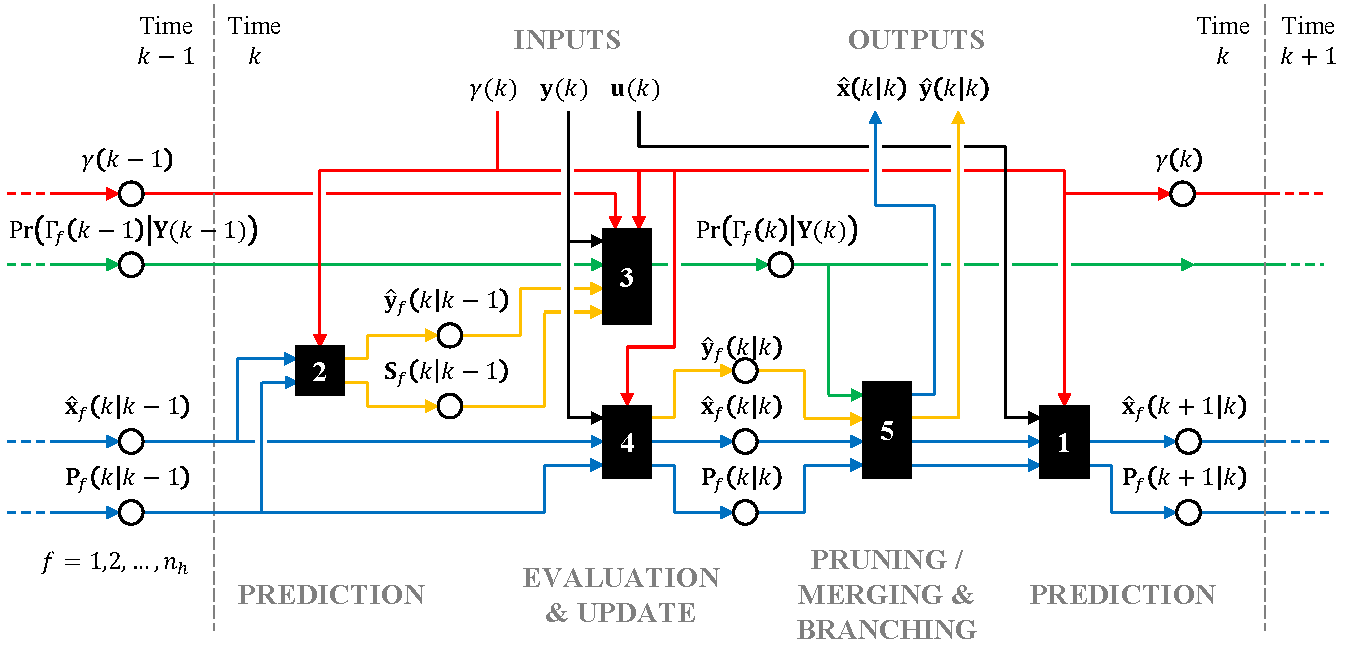
\includegraphics[width=15.5cm]{images/mkf_infoflow.pdf}
	\caption{General information flow diagram of a multiple-model observer}
	\label{fig:mkf-infoflow}
\end{figure}

At time $k$, the algorithm requires a mode indicator vector, $\gamma(k)=\begin{bsmallmatrix} \gamma_1(k) & \cdots & \gamma_{n_h}(k) \end{bsmallmatrix}^\intercal$, the system output measurement, $\mathbf{y}_M(k)$, and input, $\mathbf{u}(k)$, and produces estimates of the states, $\hat{\mathbf{x}}(k \mid k)$, and outputs, $\hat{\mathbf{y}}(k \mid k)$. The mode indicator vector is either constant, as in the case of the \gls{GPB1} and \gls{GPB2} algorithms or is specified by the sub-optimal procedure at each time step. At the end of each time step, the mode indicator vector, conditional hypothesis probabilities, one-step-ahead state predictions, and the prediction error covariances for each hypothesis are stored for use in the next time step. The sub-optimal algorithm, which determines $\gamma(k)$ as well as the merging, pruning, and branching procedures in step 6, may have other variables that need to be stored. These are not shown on the diagram. The total number of hypotheses modelled, $n_h$, also depends on the algorithm, and may be time-varying.

\section{System identification} \label{sec:sys-id}

% Some text not used in IFAC report
Model-based observers such as the Kalman filter require a dynamic model of the process. In practice, models of the process dynamics are not available but they can be identified when input-output data sampled from the process is available. In this case, system identification methods are common practice, as described by \cite{ljung_system_1999} among others.

To construct a multiple-model observer for systems with \gls{RODD}s, the structure and parameters of the disturbance model as well as the process model are needed. \gls{RODD}s are discrete-time \acrlong{MJLS} (\acrshort{MJLS}) \citep{costa_discrete-time_2005}. Standard approaches to system identification such as least-squares regression are not applicable to hybrid dynamical systems with both discrete and continuous states. Identification of these types of systems is challenging and the subject of ongoing research. See for example, \cite{piga_estimation_2020}.

%Outline notes:
%\begin{itemize}
%	\item Explain Isaksson and Eriksson's perspective on standard system identification approach.
%	\item Explain distinction between system detection or `discrimination' and system identification, reference Isaksson and Eriksson's paper on disturbance classification (whether disturbance at input or output of process).
%	\item Introduce other approaches—MLE, EM algorithm (Dempster et al., Wong \& Lee)
%	\item Methods proposed by Bemporad (Fitting jump models, 2018 and Jump Box-Jenkins, 2020).
%	\item Theory and challenges Costa book. Others?
%	\item In recent years, numerical methods to overcome the intractability of the probabilistic integral have received a lot of attention.
%	\item Sequential Monte-Carlo methods, (incl. particle filtering), Stochastic Variational Inference, ... (read Special issue in IEEE control magazine for an overview of these methods)
%\end{itemize}

% More text from IAFAC paper:
%are assumed to be known and were set to match the characteristics of the simulated disturbance. In practice, they would have to be estimated, either using prior knowledge of the disturbance source, or possibly from system output measurements using an appropriate system identification method---see \cite{schon_sequential_2015} for one possible approach---provided a sufficiently long sequence of data is available.

% Note: may remove this if we aren’t using any formal methods.

%\section{Control strategies}
%
%In this work, the goal is to test the performance of different observers in a closed-loop feedback control application (not to evaluate different control strategies). Therefore, only one control strategy is considered. According to the \textit{separation principle} of estimation and control, the control strategy may be designed independently of the observer. The controller is designed using the same augmented system model, including the plant model and disturbance models, that is used in the observer design. However, the switching behaviour of the random shock variable used in the \gls{RODD} is not explicitly considered in the control design. The estimates of the model states produced by the observer are assumed to be optimal, i.e. the expected values, and their uncertainty is not taken into account by the control algorithm or in its design.
%
%
%\subsection{Model predictive control}
%
%\textit{\acrlong{MPC}} (\acrshort{MPC}) is a well known and widely used multi-variable control algorithm used in industrial applications. This is largely due to the fact that constraints can be imposed on the manipulated variables and control variables, as well as its intuitive design and the ease with which it can be tuned to achieve control objectives \citep{maciejowski_predictive_2002}. Although it is a computationally complex algorithm, numerous proven commercial products exist to enable its implementation.
%
%\gls{MPC} utilizes a prediction equation based on the dynamic model of the system to find feasible future trajectories of the system outputs as a function of the manipulated variables and the states of the model at the current time. The length of the prediction horizon, \gls{Hp}, is defined in terms of the number sample times starting at the next time instant, $k+1$. The predicted outputs over the prediction horizon, calculated at the current time $k$, are denoted $\hat{\textbf{y}}(k+i | k)$ for $i=1,2,...,H_p$. The length of the control horizon, \gls{Hc}, is defined starting at the current time, $k$, and the manipulated inputs are denoted $\mathbf{u}(k+i-1)$ for $i=1,2,...,H_c$. The control horizon is usually shorter than the prediction horizon, in which case, $\mathbf{u}(k+j)=\mathbf{u}(k+H_c-1)$ for $j=H_c,H_c+1,...,H_p$.
%
%The constrained optimization problem, which is solved at each time step, is
%\begin{align} \label{eq:mpc-opt}
%	\begin{split}
%		\min _{\mathbf{u}(k), \mathbf{u}(k+1), \ldots, \mathbf{u} (k+H_c-1)}
%		& \quad \sum_{i=1}^{H_{p}}[\mathbf{\hat{y}}(k+i / k) - \mathbf{r}(k+i)]^\intercal \mathbf{\Phi} [\mathbf{\hat{y}}(k+i / k) - \mathbf{r}(k+i)] \\
%		& \qquad + \sum_{i=1}^{H_{c}}[\Delta \mathbf{u}(k+i-1)]^\intercal \mathbf{\Lambda} [\Delta \mathbf{u}(k+i-1)] \\
%			\end{split} \\
%		\text { subject to: }
%		&\ \mathbf{u}_{min} \leq \mathbf{u}(k+j-1) \leq \mathbf{u}_{max} \quad  j=1,2, \dots, H_{c} \label{eq:mpc-cons-1}, \\
%		& \Delta \mathbf{u}_{min} \leq \Delta \mathbf{u}(k+j-1) \leq \Delta \mathbf{u}_{max} \quad j=1,2, \dots, H_{c}, \label{eq:mpc-cons-2} \\
%		& \mathbf{y}_{min} \leq \mathbf{\hat{y}}(k+j / k) \leq \mathbf{y}_{max} \quad  j=1,2, \dots, H_{p}, \label{eq:mpc-cons-3}
%\end{align}\textbf{[TODO: Consider including slack variables to ensure feasibility]}
%where $\mathbf{r}(k+i)$ for $i=1,2,...,H_p$ is the reference output trajectory, and $\Delta \mathbf{u}(k)$ is the change in the manipulated variable at time $k$, defined as $\Delta \mathbf{u}(k) = \mathbf{u}(k) - \mathbf{u}(k-1)$. The tunable parameters are $H_p$, $H_c$, $\mathbf{\Phi}$, and $\mathbf{\Lambda}$, and the constraints are $\mathbf{u}_{min}$, $\mathbf{u}_{max}$, $\Delta \mathbf{u}_{min}$, $\Delta \mathbf{u}_{max}$, $\mathbf{y}_{min}$, and $\mathbf{y}_{max}$. Note that the last constraint \eqref{eq:mpc-cons-3} only guarantees that the estimate of the system output will not violate the constraints. This does not imply that the true system output will respect them at all times.
%
%Once a solution to the optimization problem is found, only the control actions at the current time, $\mathbf{u}(k)$, are transmitted to the plant. The procedure is then repeated every future time instant to compute the subsequent control actions. This is referred to as \textit{receding horizon control}.


\section{Grinding simulation model} \label{sec:grinding-simulator}

%Outline notes:
%\begin{outline}
%    \1 Assumptions and limitations: constant breakage rate model, relationships between speed, media, trajectories, filling level and breakage not captured.
%	\1 Describe grate, transport delays and cyclone model.
%	\1 Outline any significant changes made from Edgar's model
%	\1 Figure: simulation results showing steady-state characteristics - e.g. power, grind, and throughput vs. fill level and speed.
%	\1 Figure \ref{fig:coarse_fine_psd_plot}: Particle size distributions of feed, recirculating load and product - this should help explain steady-state characteristics.
%	\1 Figure - Step responses of main process variables to changes in ore properties.
%	\1 Selection of particle size distribution as the disturbance variable for this work.
%	\1 Steady-state characteristics with operating points (grind curves)\\
%\end{outline}

A dynamic simulation model of the primary grinding circuit of a gold mine in Quebec is used to simulate the effects of changes in ore feed properties on the grinding circuit over time. The model was developed by \cite{perez_garcia_dynamic_2020} following the methodology described by \cite{grimble_dynamic_2010} and was calibrated to match operating data collected from the plant \citep{perez-garcia_systematic_2020}. Grinding in the \acrshort{SAG} mill is simulated by a \textit{population balance model} with 24 discrete ore particle size intervals and constant specific-energy selection rates (i.e. breakage rates are proportional to total energy consumption) and a constant breakage matrix.

Figure \ref{fig:sag-diag} is a simplified diagram of the simulated \acrshort{SAG} mill, which is in a closed circuit consisting of a feed conveyor, pump box, pump, and a bank of hydro-cyclones.
\begin{figure}[ht]
	\centering
	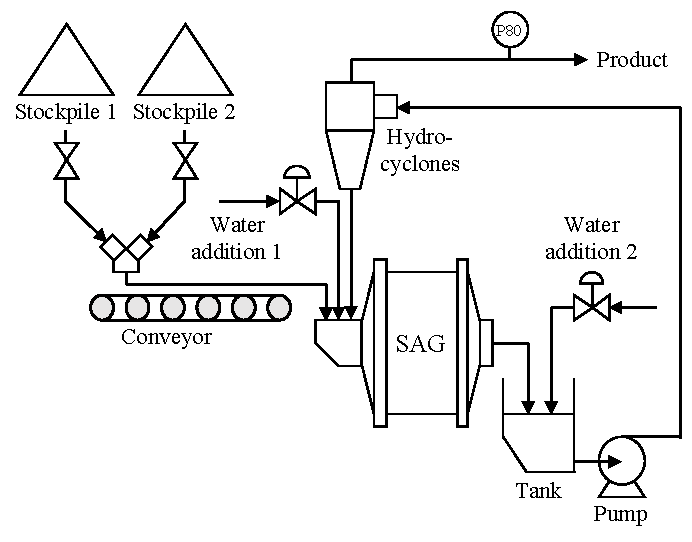
\includegraphics[width=12.5cm]{images/sag-circuit-diag.pdf}
	\caption{Simplified process flow diagram}
	\label{fig:sag-diag}
\end{figure}
For the purposes of this work, two ore feed streams with different \gls{PSD}s were simulated. Each stream is a different mix of two different ores. One ore has a fine \gls{PSD} and the other is coarse. The mix for stream \#1 (`mix 1') consists of 22.83\% coarse ore (\textit{mix factor} of 0.2283) and mix \#2 is an even mix of both ores (mix factor of 0.5). The two streams are mixed before discharging onto the conveyor. Figure \ref{fig:coarse_fine_psd_plot} shows the \gls{PSD}s of the two mixtures.
\begin{figure}[ht]
	\centering
	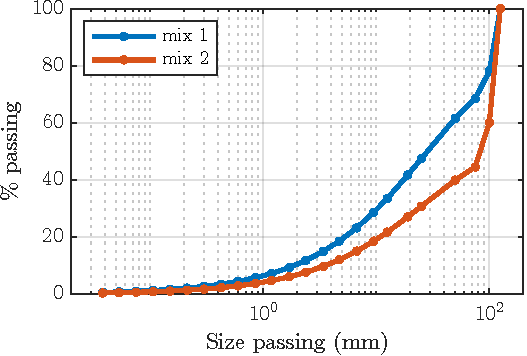
\includegraphics[width=9cm]{images/coarse_fine_cumpsd_plot.pdf}
	\caption{Ore particle size distributions}
	\label{fig:coarse_fine_psd_plot}
\end{figure}

The simulated instrumentation is also illustrated in Figure \ref{fig:sag-diag}. \hl{The setpoint of the water addition flowrate to the mill inlet (`water addition 1') is set to a fixed ratio of the ore feed rate.} The pump-box \hl{(`tank')} has a \gls{PI} controller to control the level to a fixed set-point by manipulating the water addition flow rate set-point (`water addition 2'). The main process variable used in this work is the product P80 measurement, which is a simulated online analyser that estimates the 80\% passing size of the material \hl{in the slurry} leaving the circuit. In this work, the inlet water addition ratio, the conveyor speed, the discharge pump speed, and the mill rotational speed are all fixed.

%The simulated instrumentation is also illustrated in Figure \ref{fig:sag-diag}. The \acrshort{SAG} mill water addition set-point is set by ratio control to a fraction of the fresh ore feed rate, which is measured on the conveyor. This water addition ratio is also manipulated. The pump-box level has a PI (proportional-integral) controller to control the level to a fixed set-point by manipulating the water addition flow rate set-point. The discharge pump speed is fixed. Conveyor speed is adjusted automatically in response to the fresh ore feed rate set-point. The \acrshort{SAG} rotational speed set-point may also be manipulated.
%
%The measurable process variables used in this work are the mill weight, which includes the weight of the shell and liners as well as the mill contents, mill power consumption, the solids-content of the cyclone feed stream, and the particle size (P80) of the ground product in the cyclone overflow. Mill filling level and other simulation variables are available for analysis but are assumed to be unmeasured in the real operation and therefore not available for process control.  Figure \ref{fig:grind_sim_io_diag} summarizes the inputs and outputs of the simulation model. Table \ref{tb:grind-vars} lists the normal operating points, units, and minimum and maximum operating limits of each variable.
%
%%TODO: Table of process variables and normal operating points, limits etc.
%\begin{table}[ht]
%	\centering
%	\caption{Grinding simulation model inputs and outputs} \label{tb:grind-vars}
%	% See: https://texblog.org/2019/06/03/control-the-width-of-table-columns-tabular-in-latex/
%	% Also: https://www.overleaf.com/learn/latex/Tables
%	\begin{tabular}{c c >{\raggedright}p{5.5cm} c c c c}
%		%\toprule
%		& Label & Description & Op. pt. & Units & Min. & Max \\
%		\midrule
%		\multicolumn{7}{l}{\textit{manipulated variables}} \\
%		%\midrule
%		  & MV1       & Ore feed rate & 122.7 & tons/h & 0 & 200 \\   
%		  & MV2       & Mill speed (fraction of critical speed) & 0.77 & - & 0 & 0.85 \\ 
%		  & MV3       & Water addition ratio (fraction of ore feed rate) & 0.341 & - & 0 & 1 \\ 
%		%\midrule
%		\multicolumn{7}{l}{\textit{Unmeasured disturbance input}} \\
%		%\midrule
%		  & UD1        & Ore mix factor & 0.2283 & - & 0 & 1  \\ 
%		%\midrule
%		\multicolumn{7}{l}{\textit{Output variables}} \\
%		%\midrule
%		  & OV1        & Mill weight & 279.4 & tons & 100 & 320  \\ 
%		  & OV2       & Mill power consumption & 2391 & kW & 0 & 2400  \\ 
%		  & OV3       & Cyclone feed solids fraction & 61.4 & \% & 50 & 70  \\ 
%		  & OV4       & Cyclone overflow P80 & 105.4 & \% & 0 & 200  \\ 
%		\bottomrule
%	\end{tabular}
%\end{table}

%To better understand the relationships between the input and output variables, a set of simulations were carried out to determine steady-state operating conditions in the vicinity of the normal operating point. Figure \ref{fig:grind_sim_ss_plot1} shows how the steady-state values of the four output variables are affected by changes in the mill fill level (fraction of internal volume occupied by the charge) and rotation speed. The normal operating points are also shown, represented by solid markers. For these simulations, a simple PI controller was used to control the mill filling level by manipulating the ore feed rate and each simulation was run until all variables converged to steady-state values. However, no constraints were imposed during these simulations, therefore power consumption exceeds the maximum possible in some cases.
%
%These results are equivalent to the grind curves proposed by \cite{powell_applying_2009} for evaluating steady-state characteristics and optimal operating points for \acrshort{SAG} mills. However, compared to the curves presented by \cite{powell_applying_2009}, which were based on measurements from real operations, these are noticeably much closer to straight lines (i.e. linear relationships).
%
%A similar set of simulations were carried out to understand the effect of changing the ore mix factor on the steady-state values of the output variables. The results are shown in Figure \ref{fig:grind_sim_ss_plot2}. From these it can be seen that the change in ore mix has no effect on the steady-state power consumption of the mill. However, there are changes in the steady-state throughput (ore feed rate), cyclone feed solids fraction, and product particle size. The throughput is approximately 4 tons-per-hour higher and the product particle size is 1.5 microns smaller when the ore mix contains the higher fraction (0.5) of coarse ore.
%
%\begin{figure}[ht]
%	\centering
%	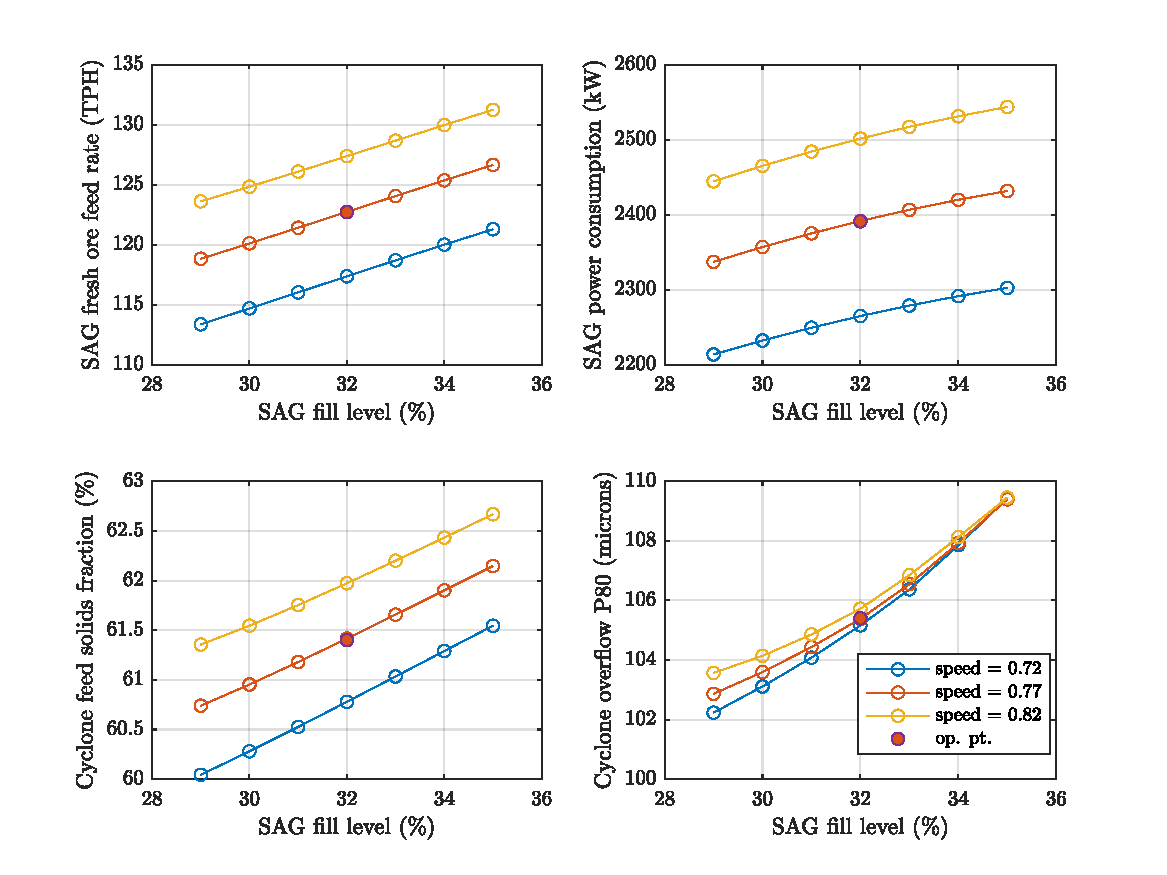
\includegraphics[width=15cm]{images/grind_sim_ss_plot1.pdf}
%	\caption{Steady-state operating points}
%	\label{fig:grind_sim_ss_plot1}
%\end{figure}
%
%\begin{figure}[ht]
%	\centering
%	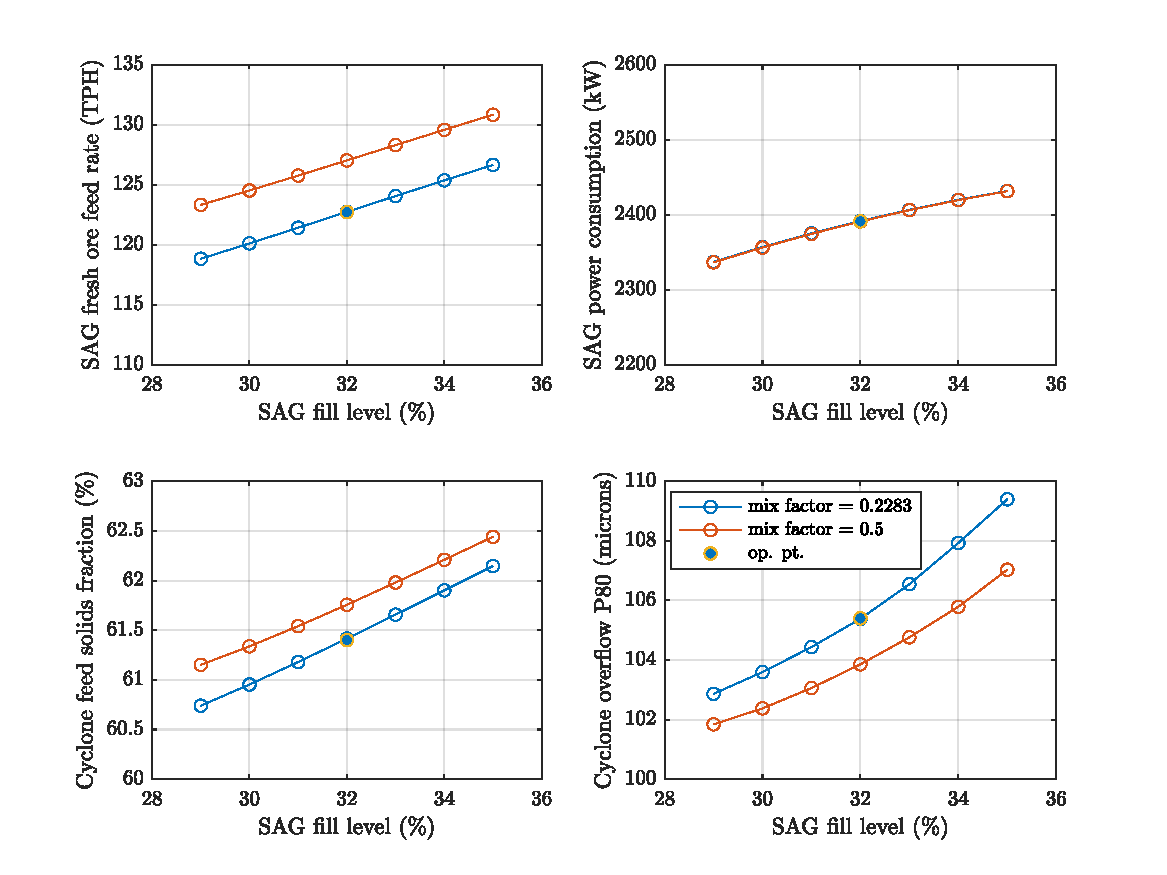
\includegraphics[width=15cm]{images/grind_sim_ss_plot2.pdf}
%	\caption{Effect of ore mix factor on steady-state operating points}
%	\label{fig:grind_sim_ss_plot2}
%\end{figure}

%Zero-mean Gaussian measurement noises are added to the outputs of the simulation model to simulate measurement errors. The standard deviations of these noises are shown in Table \ref{tb:meas-noise}. Except for the measurement noises and the input disturbance described above, the model itself is deterministic.

% Scaling factors
% 2
%& 0.0085
%& 0.01
%& 0.01
%& 2.2
%& 24
%& 0.2
%& 2
%
%\begin{table}[h!]
%	\centering
%	\caption{Simulated output measurements} \label{tb:meas-noise}
%	\begin{tabular}{c >{\raggedright}p{5.5cm} c c}
%		Label & Description & Sampling period (hours) & Noise std. dev. \\
%		\midrule
%		CV1        & Mill weight & 0.05 & XX \\ 
%		CV2       & Mill power consumption & 0.05 & XX \\ 
%		CV3       & Cyclone feed solids fraction & 0.05 & XX \\ 
%		CV4       & Cyclone overflow P80 & 0.05 & XX \\ 
%		\bottomrule
%	\end{tabular}
%\end{table}
%
%
%Although some of these process variables would likely be sampled at higher rates in practice, it is assumed, for simplicity, that they are all sampled at the same rate of 1 sample every 3 minutes (i.e. a sampling period of 0.05 hours). This was deemed to be a typical sampling rate of a standard online particle size analyser that might be used for the P80 measurement.


\section{Performance evaluation} \label{sec:evaluation}

Various metrics are used in this work to evaluate the performance of the observers. Since a simulation model of the plant is used and the input disturbances are also simulated, the true values of the system inputs and outputs (i.e. without measurement errors) are available.

The first metric is the \textit{\acrlong{RMSE}} (\acrshort{RMSE}) of the system output estimates, which is an indication of the magnitude of the differences between the estimates of an output signal, $\hat{Y}_i(N)=\left\{\hat{y}_i(1),\hat{y}_i(2), ..., \hat{y}_i(N)\right\}$, and its true values, $Y_i(N)=\left\{y_i(1),y_i(2), ..., y_i(N)\right\}$, (i.e. the output estimation errors),
\nomenclature{$\hat{Y}_i(k)$}{estimates of system output $i$ from time 0 to time $k$}%
\nomenclature{$\hat{\mathbf{Y}}(k)$}{system output estimates from time 0 to time $k$}%
\nomenclature{$Y_{i}(k)$}{system output $i$ from time 0 to time $k$}%
\nomenclature{$Y_{M,i}(k)$}{measurements of system output $i$ from time 0 to time $k$}%
\nomenclature{$\mathrm{RMSE}(\hat{Y},Y)$}{\acrlong{RMSE} of the output estimates, $\hat{Y}(N)$, from a simulation, compared to the true system outputs, $Y(N)$}%
\nomenclature{$\mathrm{RMSE}(\hat{Y},Y_M)$}{\acrlong{RMSE} of the output estimates, $\hat{Y}(N)$, from a simulation, compared to the system output meaurements, $Y_M(N)$}%
\begin{equation} \label{eq:rmse-calc-yest}
	\newcommand{\RMSE}{\textrm{RMSE}}
	\RMSE(\hat{Y}_i(N),Y_i(N)) = \sqrt{\frac{1}{N}\sum_{k=1}^{N}{(\hat{y}_i(k)-y_i(k))^2}}.
\end{equation}

Similarly, the \gls{RMSE} of the estimates of an unmeasured input disturbance signal, $\hat{p}_i(k)$, is
\begin{equation} \label{eq:rmse-calc-pest}
	\newcommand{\RMSE}{\textrm{RMSE}}
	\RMSE(\hat{P}_i(N),P_i(N)) = \sqrt{\frac{1}{N}\sum_{k=1}^{N}{(\hat{p}_i(k)-p_i(k))^2}}.
\end{equation}
 
As well as the overall \gls{RMSE}, two additional metrics are used to evaluate observer performance on systems with \gls{RODD}s. The \gls{RMSE} \textit{in transition}, which is the \gls{RMSE} during a period after a random shock, is used to evaluate the response of an observer to infrequent, abrupt disturbances. The transition period is defined as the samples occurring within $t_{\pm5\%}$ hours of the disturbance arriving at the input to the process, where $t_{\pm5\%}$ is the \textit{settling time} \hl{of the process}, defined as the time taken for the outputs to converge to within $\pm5\%$ of the final steady-state values. The \gls{RMSE} \textit{in steady-state} is defined as the samples occurring more than $t_{\pm5\%}$ hours after a disturbance and before the next one occurs.
\nomenclature{$t_{\pm5\%}$}{settling time of the process to within $\pm5$ percent of steady-state}%

The fourth metric is the \textit{\acrlong{RMSD}} (\acrshort{RMSD}) in the estimates,
\nomenclature{$\mathrm{RMSD}(\hat{Y})$}{\acrlong{RMSD} of the output estimates, $\hat{Y}(N)$, from a simulation}%
\begin{equation} \label{eq:rmsd-calc-yest}
	\newcommand{\RMSD}{\textrm{RMSD}}
	\RMSD(\hat{Y}_i(N)) = \sqrt{\frac{1}{N}\sum_{k=1}^{N}{(\hat{y}_i(k)-\hat{y}_i(k-1))^2}}.
\end{equation}
\nomenclature{$\mathrm{Var}(\hat{Y})$}{Variance of the output estimates, $\hat{Y}(N)$, from a simulation}%

This is a measure of the magnitude of high frequency changes in the estimates, which is an indication of the sensitivity of an observer to measurement noise.

\hl{A fifth metric is used in the case of the grinding simulator experiments, the variance of the estimates during steady-state periods. This is similar to the {\gls{RMSE}} in that it gives an indication of the sensitivity of the estimates to measurement noise.}
% Variance calc - only used in grinding model simulations
\begin{equation} \label{eq:var-calc}
	\begin{aligned}
		\newcommand{\Var}{\textrm{Var}} 
		\Var(\hat{y}(k)) = \frac{1}{N}\sum_{k=1}^{N}{(\hat{y}(k)-\mu_y)^2} \\
		\mu_y = \frac{1}{N}\sum_{k=1}^{N}{\hat{y}(k)}
	\end{aligned}
\end{equation}

To simplify notation, the argument $N$, indicating the length of the time series, is not always shown. Thus, $\textrm{RMSE}(\hat{Y}_i(N),Y_i(N))$ may be denoted $\textrm{RMSE}(\hat{Y}_i,Y_i)$. The capitalization of $Y$ indicates that it is a time series. Also, for \gls{SISO} systems, the subscript $i$ is redundant and dropped. Thus, $\textrm{RMSE}(\hat{Y},Y)$ is the \gls{RMSE} of the output of a system with only one output variable. However, $\textrm{RMSE}(\hat{\mathbf{Y}},\mathbf{Y})$ is used for a system with more than one output. The assumption is that this is the \gls{RMSE} averaged over all output signals, $Y_i(N)$ for $i=1, ..., n_y$.
% Removed since not doing control simulations.
%To evaluate the potential benefits of the observers in process control applications, simulations were carried out with an observer, a simulated controller, and the simulated process in closed-loop. In these cases, the \gls{RMSE}s of the control variables, $y_i(k)$, compared to a set of reference values, $R_i(N)$, is calculated to evaluate the performance of the control system,
%\begin{equation} \label{eq:rmse-calc-y}
%	\newcommand{\RMSE}{\textrm{RMSE}}
%	\RMSE(Y_i(N),R_i(N)) = \sqrt{\frac{1}{N}\sum_{k=1}^{N}{(y_i(k)-r_i(k))^2}}.
%\end{equation}
%
%In addition, the RMSD of the control actions, $u_i(k)$, is calculated to provide an indication of the sensitivity of the control system to measurement noise,
%\begin{equation} \label{eq:rmsd-calc-u}
%	\newcommand{\RMSD}{\textrm{RMSD}}
%	\RMSD(U_i(N)) = \sqrt{\frac{1}{N}\sum_{k=1}^{N}{(u_i(k)-u_i(k-1))^2}}.
%\end{equation}

Because the processes simulated in this work are stochastic, it is important to evaluate state estimators over sufficiently long simulation time periods to ensure that the results are close to the true average performance and are independent of the specific pseudo-random inputs generated for each simulation. This is particularly important when evaluating systems with \gls{RODD}s because the shocks occur infrequently. As an added precaution, identical random inputs are used when comparing the performance of two or more observers on the same system.

\hljb{In this chapter, the main methods and notation used in this work were introduced. The main disturbance model considered is the {\gls{RODD}} model ({\ref{eq:RODD}}), however, two additional disturbance models were presented, a more general switching model based on the HMM ({\ref{eq:MJLS}}) and the {\gls{BRW}} ({\ref{eq:brw}}). The standard Kalman filter (filtering form) was introduced, along with the multiple-model Kalman filter for estimation of switching systems. The two main sub-optimal algorithms used for {\gls{RODD}} estimation are a sequence fusion algorithm} {\citep{robertson_detection_1995, robertson_method_1998}} \hljb{(two versions of it), and a sequence pruning algorithm} {\citep{eriksson_classification_1996}}, \hljb{with implementation details. The grinding simulation model used to simulate a realistic grinding circuit was also introduced. Finally, the metrics used to evaluate the performance of observers were defined. The next chapter describes a series of simulations carried out to evaluate these observers.}